
\documentclass[a4paper]{article}
\usepackage{vntex}
%\usepackage[english,vietnam]{babel}
%\usepackage[utf8]{inputenc}

%\usepackage[utf8]{inputenc}
%\usepackage[francais]{babel}
\usepackage{a4wide,fancyhdr}
%\usepackage{a4wide,amssymb,epsfig,latexsym,array,hhline,fancyhdr}

%\usepackage[makeroom]{cancel}
\usepackage{amsmath}
\newcommand\numberthis{\addtocounter{equation}{1}\tag{\theequation}}
\usepackage{amsthm}
\usepackage{multicol,longtable,amscd}
%\usepackage{diagbox}%Make diagonal lines in tables
%\usepackage{booktabs}
%\usepackage{alltt}
\usepackage[framemethod=tikz]{mdframed}% For highlighting paragraph backgrounds
\usepackage{caption,subcaption}
%\usepackage{arydshln}
\usepackage{tabularx} % in the preamble
\usepackage{tikz}
%\usetikzlibrary{positioning}
\usetikzlibrary{shapes, calc, shapes, arrows}
\usepackage{pgfplots}
\usepackage{bbm}
%\usetikzlibrary{calc,positioning,shadows.blur,decorations.pathreplacing}
%\usepackage{etoolbox}
\DeclareMathOperator*{\argminB}{argmin} 
\DeclareMathOperator*{\argmaxB}{argmax} 

%\setlength\dashlinedash{1.5pt}
%\setlength\dashlinegap{4.5pt}
\setlength\arrayrulewidth{0.2pt}

\usepackage{textcomp}
%\usepackage{listings}
%\usepackage{listingsutf8}
% Typesetting Listings
\usepackage{xcolor}
\usepackage{color}
%\definecolor{listinggray}{gray}{0.9}
%\definecolor{lbcolor}{rgb}{0.9,0.9,0.9}
%\definecolor{Darkgreen}{rgb}{0.1,0.6,0.1}
%
%\lstset{
%	backgroundcolor=\color{lbcolor},
%	tabsize=4,    
%	%   rulecolor=,
%	language=[GNU]C++,
%	basicstyle=\scriptsize,
%	upquote=true,
%	aboveskip={1.5\baselineskip},
%	columns=fixed,
%	showstringspaces=false,
%	extendedchars=false,
%	breaklines=true,
%	prebreak = \raisebox{0ex}[0ex][0ex]{\ensuremath{\hookleftarrow}},
%	frame=single,
%	numbers=left,
%	showtabs=false,
%	showspaces=false,
%	showstringspaces=false,
%	identifierstyle=\ttfamily,
%	keywordstyle=\color[rgb]{0,0,1},
%	commentstyle=\color[rgb]{0.026,0.112,0.095},
%	stringstyle=\color[rgb]{0.627,0.126,0.941},
%	numberstyle=\color[rgb]{0.205, 0.142, 0.73},
%	%        \lstdefinestyle{C++}{language=C++,style=numbers}’.
%}
%\lstset{
%	backgroundcolor=\color{lbcolor},
%	tabsize=4,
%	language=C++,
%	captionpos=b,
%	tabsize=3,
%	frame=lines,
%	numbers=left,
%	numberstyle=\tiny,
%	numbersep=5pt,
%	breaklines=true,
%	showstringspaces=false,
%	basicstyle=\footnotesize,
%	%  identifierstyle=\color{magenta},
%	keywordstyle=\color[rgb]{0,0,1},
%	commentstyle=\color{Darkgreen},
%	stringstyle=\color{red}
%}

\usepackage{lastpage}
\usepackage[lined,boxed,commentsnumbered]{algorithm2e}
\usepackage{enumerate}
\usepackage{graphicx}							% Standard graphics package
\usepackage{array}
\usepackage{tabularx, caption}
\usepackage{multirow}
\usepackage{multicol}
\usepackage{rotating}
\usepackage{graphics}
%\usepackage{geometry}
%\usepackage{setspace}
\usetikzlibrary{arrows,snakes,backgrounds}
\usepackage[unicode]{hyperref}
\hypersetup{urlcolor=blue,linkcolor=black,citecolor=black,colorlinks=true} 
%\usepackage{pstcol} 								% PSTricks with the standard color package
\usepackage{verbatim}
\usepackage{makecell}

\newtheorem{theorem}{{\bf Định lý}}
\newtheorem{property}{{\bf Tính chất}}
\newtheorem{proposition}{{\bf Mệnh đề}}
\newtheorem{corollary}[proposition]{{\bf Hệ quả}}
\newtheorem{lemma}[proposition]{{\bf Bổ đề}}
\theoremstyle{definition}
\newtheorem{exer}{Bài toán}


%\usepackage{fancyhdr}
\setlength{\headheight}{40pt}
\pagestyle{fancy}
\fancyhead{} % clear all header fields
\graphicspath{ {Images/} }
\fancyhead[L]{
	\begin{tabular}{rl}
		\begin{picture}(25,15)(0,0)
		\put(0,-8){
\includegraphics[width=8mm, height=8mm]{Images/hcmut.png}}
		%\put(0,-8){\epsfig{width=10mm,figure=hcmut.eps}}
		\end{picture}&
		%
\includegraphics[width=8mm, height=8mm]{hcmut.png} & %
		\begin{tabular}{l}
			\textbf{\bf \ttfamily Trường Đại Học Bách Khoa Tp.Hồ Chí Minh}\\
			\textbf{\bf \ttfamily Khoa Khoa Học và Kỹ Thuật Máy Tính}
		\end{tabular} 	
	\end{tabular}
}
\fancyhead[R]{
	\begin{tabular}{l}
		\tiny \bf \\
		\tiny \bf 
\end{tabular}  }
\fancyfoot{} % clear all footer fields
\fancyfoot[L]{\scriptsize \ttfamily Nhận dạng biểu thức toán học}
\fancyfoot[R]{\scriptsize \ttfamily Trang {\thepage}/\pageref{LastPage}}
\renewcommand{\headrulewidth}{0.3pt}
\renewcommand{\footrulewidth}{0.3pt}


%%%
\setcounter{secnumdepth}{4}
\setcounter{tocdepth}{3}
\makeatletter
\newcounter {subsubsubsection}[subsubsection]
\renewcommand\thesubsubsubsection{\thesubsubsection .\@alph\c@subsubsubsection}
\newcommand\subsubsubsection{\@startsection{subsubsubsection}{4}{\z@}%
	{-3.25ex\@plus -1ex \@minus -.2ex}%
	{1.5ex \@plus .2ex}%
	{\normalfont\normalsize\bfseries}}
\newcommand*\l@subsubsubsection{\@dottedtocline{3}{10.0em}{4.1em}}
\newcommand*{\subsubsubsectionmark}[1]{}
\makeatother

\everymath{\color{blue}}%make in-line maths symbols blue to read/check easily

\sloppy
\captionsetup[figure]{labelfont={small,bf},textfont={small,it},belowskip=-1pt,aboveskip=-9pt}
%space remove between caption, figure, and text
\captionsetup[table]{labelfont={small,bf},textfont={small,it},belowskip=-1pt,aboveskip=7pt}
%space remove between caption, table, and text

%\floatplacement{figure}{H}%forced here float placement automatically for figures
%\floatplacement{table}{H}%forced here float placement automatically for table
%the following settings (11 lines) are to remove white space before or after the figures and tables
%\setcounter{topnumber}{2}
%\setcounter{bottomnumber}{2}
%\setcounter{totalnumber}{4}
%\renewcommand{\topfraction}{0.85}
%\renewcommand{\bottomfraction}{0.85}
%\renewcommand{\textfraction}{0.15}
%\renewcommand{\floatpagefraction}{0.8}
%\renewcommand{\textfraction}{0.1}
\setlength{\floatsep}{5pt plus 2pt minus 2pt}
\setlength{\textfloatsep}{5pt plus 2pt minus 2pt}
\setlength{\intextsep}{10pt plus 2pt minus 2pt}

\newcommand{\myFrame}[2]{%
	\noindent
	\begin{tikzpicture}
	\node[inner sep=2em,draw=green!50!black,line width=1pt,
	fill=red!15, 
	text width=\dimexpr\textwidth-4em-\pgflinewidth\relax] 
	(T) {#2};
	\node[rounded rectangle, inner sep=1ex, 
	draw=green!50!black,line width=1pt,fill=green!10,
	text width=10cm,align=center,
	font=\bfseries\sffamily,
	anchor=center] 
	(H) at (T.north) {\textcolor{red}{#1}};
	%\draw (H.south west) rectangle (H.north east);
	\end{tikzpicture}%
	\par
}
\usepackage{tocbibind}
\newcommand{\listofalgorithmes}{\tocfile{\listalgorithmcfname}{loa}}

\begin{document}
	\begin{titlepage}
		
		\begin{center}
			ĐẠI HỌC QUỐC GIA THÀNH PHỐ HỒ CHÍ MINH \\
			TRƯỜNG ĐẠI HỌC BÁCH KHOA\\
			KHOA KHOA HỌC - KỸ THUẬT MÁY TÍNH\\
			
		\end{center}
		\vspace{1cm}
		
		\begin{figure}[h!]
			\begin{center}
				
\includegraphics[width=3cm]{Images/hcmut.png}
			\end{center}
		\end{figure}
		\vspace{1cm}
		
		\begin{center}
			\begin{tabular}{c}
				\multicolumn{1}{c}{\textbf{{LUẬN VĂN TỐT NGHIỆP ĐẠI HỌC}}}\\
				~~\\
				\hline
				\\
				\multicolumn{1}{c}{\textbf{{\Large
							Nhận dạng biểu thức toán học
				}}}\\
				
			\end{tabular}
		\end{center}
		
		\vspace{1cm}
		
		\begin{table}[h]
			\begin{tabular}{rrl}
				\vspace{0.5cm}
				\hspace{1.5 cm} & Hội đồng & : \bf{Khoa học máy tính}\\
				\vspace{0.5cm}
				\hspace{1.5 cm} & Giảng viên hướng dẫn & : \bf{TS. Lê Thành Sách}\\
				\vspace{0.5cm}
				\hspace{1.5cm} & Giảng viên phản biện & : \bf{TS. Nguyễn Đức Dũng}\\
				\vspace{0.5cm}
				\hspace{1.5 cm} & Nhóm sinh viên thực hiện & : \bf{Phan Tấn Phúc - 51303058}\\
				%	\vspace{0.5cm}
				\hspace{1.5 cm} & \hspace{5 cm} &  \hspace{0.15cm} \bf{Bùi Khánh Ngọc - 51302567}\\
				
			\end{tabular}
		\end{table}
		\vspace{2cm}
		\begin{center}
			{\footnotesize Tp. Hồ Chí Minh, Tháng 12/2017}
		\end{center}
	\end{titlepage}
	\newpage
	\subsection*{Lời cam đoan}
	Luận văn của nhóm có tham khảo các tài liệu từ nhiều nguồn khác nhau và các nguồn tham khảo này đều được trích dẫn rõ ràng trong phần tài liệu tham khảo. Ngoài những phần được trích dẫn, nhóm xin cam đoan toàn bộ nội dung báo cáo là do các thành viên nhóm tự soạn thảo dựa trên những tìm hiểu và kết quả thực tế do nhóm tạo ra. \\
	Thành viên nhóm sẽ hoàn toàn chịu xử lý theo quy định nếu có bất kỳ sai phạm nào xảy ra liên quan đến những gì nhóm đã cam đoan.
	\begin{table}[h]
		\begin{tabular}{lll}
			%\vspace{0.5cm}
			\hspace{8cm} Hồ Chí Minh, ngày 08 tháng 12 năm 2017\\
			\hspace{10cm}Nhóm sinh viên thực hiện\\
			%\vspace{0.5cm}
			\hspace{10.5cm}\textbf{Phan Tấn Phúc}\\
			%\vspace{0.5cm}
			\hspace{10.5cm}\textbf{Bùi Khánh Ngọc}
		\end{tabular}
	\end{table}
	
	\newpage 
	\subsection*{Lời nói đầu}
	
	Luận văn tốt nghiệp là thử thách cuối cùng của chặng đường 4.5 năm trên giảng đường đại học của những sinh viên Bách Khoa. Nó khép lại một giai đoạn mà ở đó chứa đựng đầy những nỗ lực, những phấn đấu, cả niềm vui và thỉnh thoảng là những nỗi buồn, sự luyến tiếc. Nhưng cũng từ đây một cánh cửa mới sẽ mở ra- cánh cửa của lao động, của cống hiến. 
	
	Để đi đến thời điểm này, nhóm muốn gửi lời cảm ơn chân thành đến Ban giám hiệu và các thầy cô Trường Đại học Bách Khoa Thành phố Hồ Chí Minh, cách riêng cho các thầy cô Khoa Khoa học và Kỹ thuật Máy tính đã chỉ dẫn cho các thành viên nhóm trong suốt những năm học vừa qua.
	
	Trong quá trình thực hiện luận văn, nhóm đã nhận được rất nhiều sự hỗ trợ về mặt chuyên môn cũng như những đóng góp trong vấn đề xây dựng tập dữ liệu cho đề tài từ các anh và các bạn trong và ngoài khoa Khoa học và Kỹ thuật Máy tính. Chính sự giúp sức này là động lực và cũng là sức mạnh giúp nhóm vượt qua những khó khăn trong quá trình thực hiện và đến thời điểm này có thể nói đã hoàn thành thành công. Nhóm xin bày tỏ sự cảm kích và biết ơn chân thành đến những con người này, cách riêng cho Thạc sĩ Huỳnh Chí Kiên- người anh đã luôn hỗ trợ và đưa ra những lời khuyên hữu ích bất kỳ khi nào nhóm gặp khó khăn. 
	
	Trên tất cả, lời cảm ơn chân thành nhất và sâu sắc nhất xin được gửi đến thầy hướng dẫn đề tài- Tiến sĩ Lê Thành Sách. Cảm ơn thầy đã luôn theo sát, hỗ trợ cũng như định hướng công việc cho nhóm. Cảm ơn thầy đã luôn tạo ra áp lực để thúc đẩy sinh viên của mình tiến về phía trước và cũng cảm ơn thầy vì những khi áp lực nhất đều được thầy chia sẻ. 
	
	Nhóm cũng không quên gửi lời cảm ơn đến nhóm tác giả khoá 2011\cite{qak} và tác giả Kuangliu\cite{github} vì trong quá trình thực hiện luận văn, nhóm có sử dụng mã nguồn của các tác giả này.
	
	Sau cùng, vì những hạn chế về mặt thời gian cũng như khả năng trong cách trình bày và viết báo cáo nên không thể tránh khỏi những thiếu sót, rất mong nhận được sự thông cảm và những ý kiến đóng góp từ quý thầy cô và các bạn để giúp nhóm hoàn thiện hơn.
	
	Chân thành cảm ơn.
	
	\begin{table}[h]
		\begin{tabular}{lll}
			%\vspace{0.5cm}
			\hspace{8cm} Hồ Chí Minh, ngày 08 tháng 12 năm 2017\\
			\hspace{10cm}Nhóm sinh viên thực hiện\\
			%\vspace{0.5cm}
			\hspace{10.5cm}\textbf{Phan Tấn Phúc}\\
			%\vspace{0.5cm}
			\hspace{10.5cm}\textbf{Bùi Khánh Ngọc}
		\end{tabular}
	\end{table}
	
	\newpage
	\subsection*{Tóm tắt luận văn}
	
	Luận văn  này chỉ ra quá trình thực hiện của nhóm từ tìm hiểu những kiến thức cần thiết đến hiện thực đề tài và đánh giá kết quả đạt được. Bố cục của luận văn gồm 6 chương, không kể các mục lục, phụ lục khác. 
	
	Chương 1 là chương giới thiệu tổng quan đề tài. Ở đó sẽ trình bày nhu cầu của đề tài trong xã hội cũng như đưa ra lý do vì sao nhóm chọn đề tài này và sau cùng là quá trình thực hiện của nhóm từ sau giai đoạn thực tập tốt nghiệp.
	
	Chương 2 sẽ đề cập những kiến thức liên quan trực tiếp đến đề tài mà nhóm đã tìm hiểu, cụ thể là kiến trúc mạng SSD.
	
	Chương 3 tóm lược một số công trình liên quan trực tiếp đến đề tài. Trong mục này, nhóm sẽ giới thiệu 4 công trình là cơ sở tham khảo cho quá trình hoàn thiện luận văn. 
	
	Chương 4 trình bày về phương pháp đã được sử dụng để hiện thực đề tài luận văn. Phương pháp này được xây dựng dựa trên những kiến thức đã tìm hiểu được trình bày ở chương 2 và những công trình được giới thiệu ở chương 3.
	
	Chương 5 chỉ ra quá trình hiện thực đề tài bao gồm chuẩn bị tập dữ liệu, xây dựng hệ thống và chương trình thử nghiệm. Cụ thể, nhóm sẽ diễn giải về cách cấu hình, các thông số trong từng giai đoạn của quá trình nhận dạng. Tiếp theo, nhóm sẽ giới thiệu cách thức thu thập dữ liệu cùng một số mô tả cho tập dữ liệu hiện tại mà nhóm đang sử dụng. Cuối cùng là kết quả từ chương trình thử nghiệm và những so sánh, đánh giá giữa các phiên bản được tạo ra từ việc thay đổi một số yếu tố liên quan đến quá trình nhận dạng. 
	
	Chương 6 đánh giá tổng kết luận văn. Nhóm sẽ nêu lên những điều còn tồn đọng và những điểm nổi bật, cũng như hướng phát triển tiếp theo của đề tài. Ngoài ra, sẽ là một vài dòng đúc kết lại chặng đường thực hiện luận văn tốt nghiệp của các thành viên nhóm: những điều đã học được, cảm xúc khi hoàn thành đề tài luận văn.
	\newpage
	\tableofcontents
	\newpage
	\listoffigures
	\newpage
	\listoftables
	\newpage
	
	\subsection*{Danh mục từ viết tắt}
	
	
	
	\begin{table} [!htb]
		\centering
		\begin{tabular}{| m{4cm} | m{12cm}|}\hline
			\multicolumn{1}{|c|}{\textbf{Thuật ngữ}} & 
			\multicolumn{1}{|c|}{\textbf{Giải thích}}\\\hline
			CNN & Mạng nơron tích chập (Convolutional Neural Network)\\\hline
			FCN & Mạng nơron tích chập đầy đủ (Fully convolutional netwrok) \\\hline
			SSD & Single Shot Mutilbox Detector\\\hline
			BST & Cây ngữ pháp dựa trên đường cơ sở (Baseline Syntax Tree)\\\hline
			DRACULAE & Diagram Recognition Application for Computer Understanding of Large Algebraic Expressions\\\hline
			%& t\\\hline
		\end{tabular}
	\end{table}
	
	\newpage
	\section{Giới thiệu}
	\subsection{Giới thiệu đề tài}
	\label{subsec: introduce}
	Khoa học công nghệ phát triển đồng nghĩa với việc xã hội "trở nên tự động hoá" bởi lẽ con người ngày càng có nhu cầu tìm kiếm sự hỗ trợ từ các thiết bị công nghệ và hạn chế dùng sức lực của chính mình. Dựa trên nền tảng công nghệ và nhu cầu của xã hội, hàng loạt những thiết bị, ứng dụng công nghệ ra đời. Chúng phục vụ nhu cầu của con người trong đời sống hằng ngày cũng như trong hầu hết mọi lĩnh vực của xã hội từ giao thông, y tế, thương mại,... đến giáo dục. Trong lĩnh vực y tế, phải kể đến ứng dụng giám sát sức khoẻ người dùng trên những chiếc đồng hồ thông minh của Apple hay SamSung. Với giao thông, những ứng dụng chỉ đường, định vị và giám sát xe đề phòng trộm ngày càng phổ biến và giúp ích thực sự cho con người. Riêng với giáo dục, vấn đề thường gặp đối với các bạn học sinh là giải, trực quan hoá các phương trình, hàm số toán học hay soạn các giáo án chứa nhiều công thức, ký hiệu phức tạp đối với thầy cô. Họ cần một giải pháp nào đó giúp giảm thiểu công sức trong những tình huống như vậy. Giải pháp này cần phải giải quyết những vấn đề cơ bản sau:
	
	\begin{itemize}
		\item Số hoá các công thức in trong sách hay được viết tay.
		\item Giải tham khảo một số dạng phương trình.
		\item Trực quan hoá các hàm số
		\item Biểu diễn công thức, ký hiệu viết tay dưới những lệnh mà các trình soạn thảo toán có thể hiểu được, ví dụ Latex.
		\item ...
		
	\end{itemize}
	
	
	
	\subsection{Lý do chọn đề tài}
	Bởi sự cần thiết về một ứng dụng nhận dạng biểu thức toán học đã được trình bày ở mục \ref{subsec: introduce}, trên thị trường cũng đã xuất hiện nhiều sản phẩm như vậy, đáng chú ý là PhotoMath\footnote{Một ứng dụng về nhận dạng và giải các biểu thức toán học nổi bật trên Google Play.}. Tuy nhiên, nhóm nhận thấy thách thức nếu phải hiện thực thành công đề tài này. Một số câu hỏi đã được đặt ra:\\
	\begin{itemize}
		\item Làm sao có thể nhận dạng được các ký hiệu?
		\item Làm cách nào để nhận dạng cả một biểu thức?
		\item Làm sao biết được đây là loại biểu thức gì?
		\item Liệu có chắc chắn bất kỳ những gì mình viết ra đều được hiểu đúng? 
		\item Nhóm có thể tạo ra được một sản phẩm hoàn thiện như PhotoMath không?
		
	\end{itemize}
	
	Để tự mình trả lời những câu hỏi đó, nhóm quyết tâm thực hiện đề tài này. Ngoài ra, việc áp dụng kiến thức đã học để tạo ra một sản phẩm vừa cần thiết cho xã hội vừa tự bản thân mình có thể sử dụng được tạo cho nhóm một động lực đế tiến hành. 
	
	\subsection{Phạm vi đề tài}
	
	\begin{itemize}
		\item Nhận dạng biểu thức toán học viết tay dạng offline\footnote{Nhận dạng từ ảnh chứa biểu thức toán học.}.
		\item Chuyển biểu thức từ dạng hình ảnh sang dạng máy có thể hiểu được (Latex).
		%\item Ảnh nhận diện ít nhiễu và không bị xoay quá nhiều.
		%\item Nhận diện được các cấu trúc đơn giản (tích phân, tổng, chỉ số trên, chỉ số dưới, phân số, giới hạn, ...)
		
	\end{itemize}
	
	\subsection{Quá trình thực hiện}
	Bước 1: Tìm hiểu những công trình trong nước và nước ngoài liên quan đến vấn đề nhận dạng biểu thức toán học.
	\begin{itemize}
		\item Mục tiêu: 
		\begin{itemize}
			\item Biết được khả năng giải quyết vấn đề của các hệ thống nhận dạng biểu thức toán học đã được xây dựng.
			\item Hiểu được phương pháp mà các nhóm tác giả sử dụng để thực hiện công trình của họ.
		\end{itemize}
		\item Công việc: 
		\begin{itemize}
			\item Tìm kiếm và chọn lọc những bài báo với nội dung nhận dạng biểu thức toán học.
			\item Đọc và nghiên cứu các thông tin được cung cấp bởi các bài báo.
			\item Tải mã nguồn (nếu có), chạy thử nghiệm.
		\end{itemize}
	\end{itemize}
	Bước 2: Chọn ra một phương pháp trong các phương pháp đã đọc để hiện thực.\\
	\begin{itemize}
		\item Mục tiêu: 
		\begin{itemize}
			\item Xây dựng từ đầu một hệ thống nhận dạng biểu thức toán học theo phương pháp đề xuất.
			\item Kiểm chứng độ chính xác được nêu trong bài báo và thực tế nhóm làm được. Trên cơ sở đó, tiến tới việc cải tiến để thu được kết quả tốt hơn.
		\end{itemize}
		\item Công việc:
		\begin{itemize}
			\item Đọc kỹ lại bài báo đã chọn.
			\item Tìm hiểu những kiến thức được giới thiệu trong bài báo ở mức độ có thể vận dụng được.
			\item Triển khai và hiện thực phương pháp.
		\end{itemize}	
	\end{itemize}
	%\vspace{1.5cm}
	Bước 2+\footnote{2+ là phương án thay thế của bước 2. Vì trong quá trình thực hiện bước 2, nhóm không thu được kết quả như mong đợi nên dẫn tới việc chọn một cách tiếp cận khác để giải quyết vấn đề.}: Lựa chọn một phương pháp mới để giải quyết đề tài trên cơ sở mã nguồn mở đã có.
	
	\begin{itemize}
		\item Mục tiêu: 
		\begin{itemize}
			\item Có được phương án thay thế phương án cũ không khả thi.
			\item Có được chương trình thử nghiệm.
		\end{itemize}
		\item Công việc:
		\begin{itemize}
			\item Tìm và tải bộ mã nguồn liên quan đến vấn đề nhận dạng biểu thức toán học\cite{github}.
			\item Thiết lập và chạy thử mã nguồn.
			
		\end{itemize}
	\end{itemize}
	Bước 3: Đề xuất phương pháp.
	\begin{itemize}
		\item Mục tiêu:
		\begin{itemize}
			\item Quyết định phương pháp giải quyết vấn đề của nhóm.
			
		\end{itemize}
		\item Công việc:
		\begin{itemize}
			\item Thay đổi, hoàn thiện mã nguồn trên cơ sở phương pháp nhóm đề xuất.
			
		\end{itemize}
	\end{itemize}
	Bước 4: Xây dựng tập dữ liệu
	\begin{itemize}
		\item Mục tiêu:
		\begin{itemize}
			\item Có được dữ liệu phục vụ quá trình huấn luyện và kiểm thử hệ thống của nhóm.
			
		\end{itemize}
		\item Công việc:
		\begin{itemize}
			\item Liên hệ nhóm sinh viên Khoá 2011\footnote{Nhóm sinh viên này đã từng hiện thực đề tài nhận dạng biểu thức toán học} để nhận được toàn bộ tập dữ liệu của họ bao gồm ảnh của các ký tự toán học.
			\item Chuẩn bị mẫu thu và bổ sung thêm ảnh cho một số loại ký tự mới.
			\item Xây dựng bộ ảnh chứa đựng các biểu thức toán học từ đơn giản đến phức tạp.
		\end{itemize}
	\end{itemize}
	Bước 5: Cải tiến phương pháp
	\begin{itemize}
		\item Mục tiêu:
		\begin{itemize}
			\item Hoàn thiện hệ thống nhận dạng biểu thức toán học.
		\end{itemize}
		\item Công việc:
		\begin{itemize}
			\item Kết hợp kiến thức và kết quả thử nghiệm trên tập dữ liệu để tìm ra phương pháp cải tiến.
			\item Xây dựng các phiên bản thử nghiệm khác nhau dựa trên các yếu tố có thể cải tiến.
			
		\end{itemize}
	\end{itemize}
	Bước 6: Xây dựng chương trình demo và đánh giá kết quả
	\begin{itemize}
		\item Mục tiêu:
		\begin{itemize}
			\item Có kết quả đánh giá và điều chỉnh phương pháp sao cho phù hợp.
			\item Có chương trình demo cho luận văn.
		\end{itemize}
		\item Công việc:
		\begin{itemize}
			\item Xây dựng bản demo.
			\item Xem xét ưu, nhược điểm của các cải tiến dựa trên đánh giá các độ đo.
			\item Cấu hình và lựa chọn phương án cải tiến khả thi. 
		\end{itemize}
	\end{itemize}
	
	
	%%%%%%%%%%%%%%%%%%%%%%%%%%%%%%%%%%%%%%%%%%%%%%%%%
	%%%%%%%%%%%%%%%%%%%%%%%%%%%%%%%%%%%%%%%%%%%%%%%%
	
	
	\newpage
	\section{Kiến thức đã tìm hiểu}
	
	\subsection*{Mạng Single Shot Multibox Detector\cite{liu2016ssd}}
	SSD\cite{liu2016ssd} như là một mạng cải tiến của phương pháp phát hiện bằng cửa sổ trượt\footnote{Thuật ngữ tiếng Anh: Sliding Window}. Thay vì sử dụng một (một số) cửa sổ có kích thước cố định, thì SSD sinh ra một số lượng hữu hạn các \textbf{default box} \footnote{Tiếng việt: Ô chuẩn} để rồi từ các default box đó để hệ thống có thể xác định vị trí các ký tự cần nhận diện cho quá trình huấn luyện, qua đó mạng cần phải học cách dự đoán cả kích thước của các \textbf{bounding box}\footnote{Tiếng việt: Ô Bọc} quanh ký tự thay vì chỉ chấp nhận kích thước cho trước. SSD\cite{liu2016ssd} cũng sử dụng các lớp tích chập\footnote{Thuật ngữ tiếng Anh: Convolution layer} (hay cụ thể hơn là các mạng nơ-ron tích chập\footnote{Convolutional neural network}) để trích đặc trưng, tạo tiền đề cho việc phát hiện và phân loại ký tự. \\
	Nhóm xin phép được tách quá trình huấn luyện thành ba giai đoạn: mã hóa, phát hiện - phân loại và tính giá trị lỗi. Và song song với huấn luyện, quá trình kiểm tra, kiểm định, chạy thực tiễn cũng được chia thành ba giai đoạn: trích đặc trưng - phân loại và giải mã.
	
	\subsection{Bộ mã hóa (Encoder)}
	Bộ mã hóa chỉ được sử dụng trong quá trình huấn luyện nhằm mã hóa, chuyển đổi ground truth \footnote{Thuật ngữ tiếng Anh: Ground truth} thô (được lưu trong tệp tin định dạng txt hoặc xml) sang ground truth mà mạng SSD\cite{liu2016ssd} có thể hiểu được.
	
	\subsection*{Sinh default box}
	
	Để mã hóa ground truth, bộ mã hóa trước hết có nhiệm vụ sinh ra nhiều default box có nhiều kích thước khác nhau, để làm được điều này, mạng cần phải được cung cấp một số thông số:\\
	\begin{itemize}
		\item Danh sách kích thước của các feature map (Phần này sẽ được giải thích rõ hơn ở mục sau): Mỗi feature map trong danh sách tương ứng với một mức kích thước\footnote{Thuật ngữ tiếng Anh: Scale} trong việc phát hiện ảnh. Trong một mức kích thước, tất cả các default box đều có kích thước như nhau và cách đều nhau, mỗi pixel trong feature map thể hiện một (một số default box), vì vậy, ta có thể tính được danh sách khoảng cách giữa trọng tâm giữa các default box bằng cách lấy kích thước ảnh chia cho kích thước của feature map ở mức kích thước tương ứng. Tất cả các dữ liệu liên quan đến kích thước sau đó sẽ được chuyển về tập giá trị $\{x \in R | x \in [0, 1] \} $ 
		\item Danh sách các aspect ratio\footnote{Tiếng việt: Tỉ lệ diện mạo} ứng với mỗi mức kích thước. Mạng SSD dựa vào các aspect ratio đó để tạo ra các default box có hình dạng khác nhau tại cùng một vị trí (trọng tâm của các default box có cùng một vị trí).
		\item Kích thước nhỏ nhất và lớn nhất của các default box.
	\end{itemize} 
	
	Từ những thông số trên, các default box sẽ được sinh ra theo các bước sau: \\
	Trước hết, bộ phận này tiến hành sinh ra kích thước của ổ chuẩn ứng với mỗi mức kích thước tương ứng bằng công thức: 
	\begin{align}
	s_k = s_{min} + \frac{s_{max} - s_{min}}{m - 1}(k - 1) 
	\end{align}
	Trong đó $s_{min}$ và $s_{max}$ là kích thước nhỏ nhất và lớn nhất của default box, m là số lượng feature map. Việc chọn các thông số này khá quan trọng vì nó sẽ ảnh hưởng đến các ký tự có thể nhận diện được sau này, các kích thước cần được chọn sao cho không quá lớn cũng như không quá nhỏ đối với những đối tượng được kỳ vọng nhận diện được.\\
	
	Ứng với mỗi mức kích thước:
	
	\begin{itemize}
		
		\item Mỗi default box đều được liên kết với một điểm ảnh trên feature map, ta cũng đã tính được danh sách khoảng cách trọng tâm theo đề cập ở trên. Từ đó ta dễ dàng tính được tọa độ của các trọng tâm của các default box trong ảnh theo công thức:
		\begin{align}
		(x, y) =\left( \left(i + \frac{1}{2} \right) \times step, \left(j + \frac{1}{2} \right) \times step \right)
		\end{align}
		Trong đó: $x$, $y$ là tọa độ của các trọng tâm; $i$, $j$ là các số nguyên dương nằm trong khoảng từ 0 đến kích thước feature map đang xét và $step$ là khoảng cách giữa hai trọng tâm liền kề trong mức kích thước đang xét.
		
		\item Sau khi có được tọa độ của các trọng tâm, bộ phận mã hóa tiến hành sinh các default box ứng với mỗi vị trí trọng tâm: 
		
		\begin{itemize}
			\item Tạo một default box có kích thước $s_k$ là kích thước ứng với mức kích thươc $k$ hiện tại.
			\item Tạo một default box có kích thước bằng $\sqrt{s_k \times s_{k + 1}}$\footnote{Do dùng công thức này nên với $n$ feature map thì cần sinh ra $n + 1$ giá trị $s_k$ trong khi công thức bên trên chỉ giải quyết được $n$ giá trị $s_k$ ứng với $n$ mức kích thước. Để giải quyết vấn đề này, ta có thể thêm một giá trị $s_0$ phù hợp}.
			\item Với mỗi phần tử trong danh sách aspect ratio tương ứng, ta tạo một default box có kích thước chiều rộng: 
			\begin{align}
			w = s_k \times \sqrt{aspect\_ratio}
			\end{align} 
			và chiều cao:
			\begin{align}
			h = s_k \div \sqrt{aspect\_ratio}
			\end{align}
			với $aspect\_ratio$ là aspect ratio đang xét.
		\end{itemize}
		
	\end{itemize}
	
	Như vậy, với mỗi vị trí được chọn để đặt trong tâm các default box, bộ phận mã hóa sẽ sinh ra $2 + n$ default box với $n$ là số aspect ratio ứng với mức kích thước hiện tại. Kết quả của quá trình sinh default box là một tập hợp nhiều vector. Mỗi vector ứng với một default box mang thông tin tọa độ trọng tâm, chiều dài, chiều rộng của default box.
	
	\subsection*{Matching\footnote{Thuật ngữ tiếng Anh: Matching}}
	
	Sau khi hoàn tất sinh default box, bộ phận encoder có nhiệm vụ matching dữ liệu thô là các bounding box \footnote{Thuật ngữ tiếng Anh: Bounding box} từ ground truth\footnote{Thuật ngữ tiếng Anh: Ground truth} qua các default box vừa được tạo. Kết quả là ta sẽ thu được một tập nhiều vector, mỗi vector đại diện cho mỗi default box chứa thông tin gồm tọa độ trọng tâm, kích thước của default box và nhãn của default box đó là gì (có thể là phần nền - không có gì cả, hoặc một ký tự nào đó cần được nhận diện). \\
	
	Việc matching được thực hiện bằng cách so sánh từng default box với từng bounding box trong ground truth bằng cách tính chỉ số Jaccard\cite{Jaccard}, nếu chỉ số này thỏa điều kiện thì default box đó được gán nội dung là kí tự chứa trong bounding box phù hợp nhất, nếu không thì default box được gán nội dung là "nền".\\
	
	Chỉ số Jaccard\cite{Jaccard} giữa hai bounding box được tính bằng công thức:
	\begin{align}
	J(A, B) = \frac{A \cap B }{ A \cup B }
	\end{align}
	Trong đó, A, B lần lượt là phần ảnh mà bounding box A và bounding box B chiếm. Công thức này mang ý nghĩa hai bounding box có kích thước càng tương đồng và phần trùng nhau càng nhiều thì có chỉ số Jaccard\cite{Jaccard} càng gần giá trị 1.\\
	
	\begin{center}
		\centering
		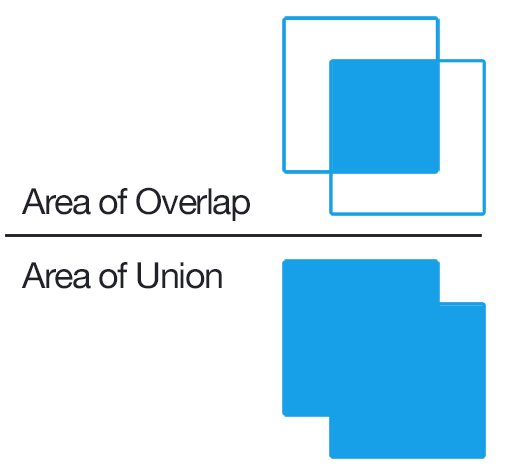
\includegraphics[width=0.5\linewidth]{Intersection_over_Union_-_visual_equation.png}
		\vspace{0.5cm}
		\captionof{figure}{Mô phỏng chỉ số Jaccard\cite{Jaccard}}
	\end{center}
	
	Các bounding box này có bản chất như một "hệ quy chiếu" cho các bounding box, sau quá trình matching, các bounding box ground truth được tính độ lệch so với các default box tương ứng và khi huấn luyện, mạng SSD\cite{liu2016ssd} có nhiệm vụ dự đoán các bounding box theo các độ lệch đó. Giá trị hàm lỗi được tính dựa trên độ lêch của bounding box ground truth và độ lệch của bounding box dự đoán được. Cách tính độ lệch sẽ được đề cập rõ hơn ở phần tính giá trị lỗi.
	
	
	\subsection{Bộ phát hiện - phân loại}
	Đây là bộ phận có nhiệm vụ trích đặc trưng từ ảnh thô đầu vào, tạo ra các feature map để đưa vào quá trình phân loại ký tự.
	
	\subsection*{Bộ phận trích đặc trưng (Hay mạng cơ sở \footnote{Thuật ngữ tiếng Anh: Base Network})}
	
	Mạng cơ sở của SSD\cite{liu2016ssd} là một mạng nơron tích chập bất kỳ, có thể là VGG\cite{Simonyan14c} hoặc lenet\cite{yanlecun},... Hầu hết những mạng này có mục đích phân loại\footnote{Thuật ngữ tiếng Anh: Classification}, vì vậy ở phía cuối mạng thường có các lớp liên kết đầy đủ nhằm giảm kích thước feature map và tạo ra dữ liệu đầu ra có kích thước phù hợp (bằng với số nhãn cần dự đoán). Khi kết hợp với mạng SSD\cite{liu2016ssd}, các lớp liên kết đầy đủ này sẽ được thay thế bằng các lớp tích chập và song hành là các bước trích ra feature map để đưa vào lớp Multibox \cite{erhan2014scalable}, chi tiết phần này sẽ được để cập ở mục tiếp theo.
	
	\subsection* {Phân loại}
	
	Bộ phận phân loại có nhiệm vụ đưa ra dự đoán về vị trí và nhãn của các ký tự có trong ảnh. Để làm được điều đó, bộ phân loại phải sinh ra các feature map ứng với từng mức kích thước khác nhau, các feature map đó được đưa vào lớp Multibox để sinh ra các vị trí dự đoán và nhãn tương ứng. Các feature map được lấy sau một (một số) lớp tích chập. Danh sách feature map có được ở giai đoạn sinh default box chính là được lấy từ đây. \\
	
	\begin{center}
		
		\centering
		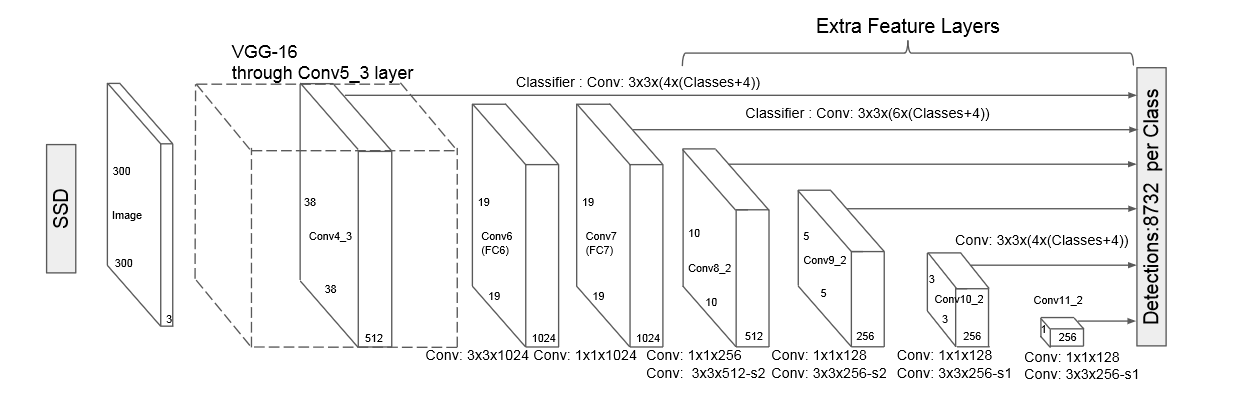
\includegraphics[width=0.8\linewidth]{SSD_Struture.png}
		\vspace{0.5cm}
		\captionof{figure}{Cấu tạo của một mạng SSD\cite{liu2016ssd}}
	\end{center}
	Sau khi có được các feature map, lớp Multibox sẽ tiến hành đưa ra dự đoán về bounding box và nhãn gắn với bounding box đó. Mỗi feature map sử dụng một tập hợp các lớp tích chập sẽ cho ra một số lượng dự đoán nhất định. Với mỗi vị trí trên feature map được kernel trượt qua, thì một dự đoán về ký tự được sinh ra. Kernel có kích thước:
	\begin{align}
	3 \times 3 \times (n \times (classes + 4))
	\end{align}
	Với $n$ là số lượng aspect ratio với fearture map tương ứng và $classes$ là số lượng nhãn cần nhận diện, số $4$ trong công thức đại diện cho 4 thông số về vị trí của bounding box (tọa độ trọng tâm và kích thước). Do kích thước của các kernel không đồng nhất (vì số lượng aspect ratio ứng với từng feature map có thể khác nhau), nên để tạo ra dữ liệu đầu ra phù hợp với các default box đã tạo từ trước thì các vector dự đoán sẽ được sắp xếp lại sao cho dữ liệu đầu ra chỉ có $classes + 4$ kênh và vị trí của các vector phải tương ứng với vị trí các default box đã sinh từ trước.
	
	\subsection{Tính giá trị lỗi}
	
	Giá trị lỗi được tính bằng tổng có trọng số giữa lỗi về vị trí\footnote{Thuật ngữ tiếng Anh: Localization Loss} và lỗi về độ tin cậy\footnote{Thuật ngữ tiếng Anh: Confidence Loss}
	\begin{align}
	L(x,c,l,g) = \frac{1}{N} (L_{conf}(x,c) + \alpha L_{loc}(x,l,g) )
	\end{align}
	Trong đó:
	\begin{itemize}
		\item x biểu thị các phép matching, cụ thể $x^p_{ij}$ biểu thị phép matching giữa default box thứ $i$ với bounding box thứ $j$ đối với nhãn $p$. Vì vậy $x^p_{ij}$ có tập giá trị $\{0, 1\}$.
		\item $c$ biểu thị nhãn kỳ vọng cho phép matching đang xét.
		\item $l$ biểu thị bounding box dự đoán.
		\item $g$ biểu thị bounding box ground truth.
	\end{itemize}
	
	Hàm lỗi về vị trí có thể được biểu diễn bằng công thức:
	\begin{align}
	L_{loc}(x,l,g) = \sum^N_{i \in Pos} \sum_{m \in \{ cx, cy, w, g \}} x^k_{ij} smooth_{L1} (l^m_i - \hat{g}^m_j)
	\end{align}
	Trong đó:
	\begin{itemize}
		\item N là số lượng phép matching giữa default box và bounding box có ý nghĩa (nhãn của phép matching không phải là "nền". Nếu như $N = 0$ thì ta đặt giá trị lỗi bằng 0.
		\item Pos là tập hợp các phép matching có ý nghĩa.
		\item $smooth_{L1}$ (theo \cite{girshick2015fast}) là một hàm tính lỗi được định nghĩa là:
		\begin{align}
		L(x) = \begin{cases} 0.5x^2 \quad if |x| < 1 \\ |x| - 0.5 \quad otherwise \end{cases}
		\end{align}
		\item \begin{align}\hat{g}_j^{cx} = (g_j^{cx} - d_i^{cx}) / d^w_i\end{align}Với $d$ biểu thị cho default box.
		\item \begin{align}\hat{g}_j^{cy} = (g_j^{cy} - d_i^{cy}) / d^h_i\end{align}
		\item \begin{align}\hat{g}^w_j = \log \left( \frac{g_j^w}{d_i^w} \right)\end{align}
		\item \begin{align}\hat{g}^h_j = \log \left( \frac{g_j^h}{d_i^h} \right)\end{align}
	\end{itemize}
	
	Bốn công thức $\hat{g}$ trên chính là độ lệch giữa ô đang xét và default box, mà nhóm đã đề cập ở mục trước.
	
	Vậy ta có thể thấy khi tính giá trại lỗi về vị trí, ta tính dựa trên sai lệch so với default box mà bounding box ground truth ban đầu match được thay vì tính lỗi trực tiếp.\\
	
	Hàm lỗi về độ tin cậy có thể được tính theo công thức:
	\begin{align}
	L_{conf}(x, c) = - \sum^N_{i \in Pos} x^p_{ij} \log (\hat{c}^p_i) - \sum_{i \in Neg} \log (\hat{c}^0_i)
	N_u	\end{align}
	
	Với \begin{align}\hat{c}_i^p = \frac{\exp{c_i^p}}{\sum_p \exp{c}_i^p}\end{align}
	
	\subsection{Bộ giải mã (Decoder)}
	
	Bản chất của bộ giải mã khá đơn giản, nó có chức năng chuyển dữ liệu các bounding box mà mạng dự đoán (tức là những bounding box được tính kích thước và tọa độ theo default box mà bounding box đó được match vào) sang dữ liệu tọa độ của ảnh (có gốc tọa độ nằm ở góc trên bên trái và tọa độ nằm trong miền $[0, 1]$. Dữ liệu này cần thiết để trực quan hóa các ký tự mà hệ thống dự đoán và để đưa vào bộ phân tích cú pháp để sinh mã Latex.
	
	\subsection{Một số vấn đề khác trong mạng SSD\cite{liu2016ssd}}
	\subsection*{Tăng cường dữ liệu\footnote{Thuật ngữ tiếng Anh: Data Augumentation}}
	
	Ngay trước quá trình matching, ảnh và các bounding box được đi qua một bước gọi là cắt ngẫu nhiên\footnote{Thuật ngữ tiếng Anh: Random Crop}. Ở bước này, ảnh được cắt đi một số phần ngẫu nhiên (có tác dụng giống như phóng to (zoom) ảnh. Điều này giúp làm đa dạng dữ liệu huấn luyện và làm giảm bớt hiện tượng overfit.
	
	
	
	%%%%%%%%%%%%%%%%%%%%%%%%%%%%%%%%%%%%%%%%%%%%%%%%%
	%%%%%%%%%%%%%%%%%%%%%%%%%%%%%%%%%%%%%%%%%%%%%%%%
	
	
	\newpage
	\section{Công trình liên quan}
	Là một phần quan trọng của hệ thống \textbf{Nhận dạng ký tự thuộc thị giác}\footnote{Thuật ngữ tiếng Anh: Optical Character Recognition, viết tắt OCR.}, nhận dạng \textbf{biểu thức toán học}\footnote{Thuật ngữ tiếng Anh: Mathematical Expression, viết tắt ME.} đã được nghiên cứu trong hơn nửa thế kỷ qua. Đã có rất nhiều công trình tiêu biểu giải quyết những vấn đề xung quanh đề tài này. Trong chương này, nhóm sẽ trình bày tóm lược về 4 công trình- là những điểm tham khảo cho hệ thống nhận dạng biểu thức toán học mà nhóm sẽ hiện thực sau này.\\
	\subsection{Tổng quan}
	Nhận dạng biểu thức toán học bao gồm 2 vấn đề chính: \textbf{nhận dạng ký tự}\footnote{Thuật ngữ tiếng Anh: Symbol recognition.} và \textbf{phân tích cấu trúc}\footnote{Thuật ngữ tiếng Anh: Structural analysis.}. Hai vấn đề này có thể được xử lý tuần tự hoặc kết hợp. Đối với hướng tiếp cận tuần tự, đầu tiên phân tách\footnote{Thuật ngữ tiếng Anh: Segmentation} ảnh chứa biểu thức toán học thành những mảnh ảnh chỉ chứa các ký tự và nhận dạng chúng. Sau đó phân tích cấu trúc 2 chiều của biểu thức toán học dựa trên kết quả phân tách và nhận dạng ký tự ở bước trước đó. Khác với phương pháp xử lý tuần tự, xử lý kết hợp mong muốn thực hiện 2 quá trình nhận dạng ký tự và phân tích cấu trúc một cách đồng thời. \\
	Quan tâm đến cách giải quyết vấn đề nhận dạng biểu thức toán học theo hướng tuần tự, nhóm có liệt kê một số công trình của các tác giả và chỉ ra phương pháp họ sử dụng cho từng giai đoạn cụ thể. Thống kê này được rút trích từ \cite{survey}.
	\begin{center}
		\begin{tabular}{||c | c | c ||} 
			\hline
			Tác giả & \makecell{  Nhận dạng ký tự } & \makecell{ Phân tích cấu trúc} \\ [0.5ex] 
			\hline\hline
			P.A.Chou&\makecell{Template matching} &\makecell{ Stochastic context-\\free grammar}\\ 
			\hline
			M.Okamoto& \makecell{Recursive projection\\ và Template matching}&\makecell{ Không parsing}\\ 
			\hline
			J.Ha&\makecell{X-Y cut và mạng nơ-ron}&\makecell{ Expression tree}\\
			\hline
			R.J.Fateman &\makecell{Template matching dựa trên \\khoảng cách Hausdorff}&\makecell{ Recursive descent parser}\\
			\hline
			H.-J.Lee và J.-S.Wang&\makecell{Kỹ thuật rút trích đặc trưng\\ và giải thuật nearest-neighborhood}&\makecell{Expression Tree}\\
			\hline
		\end{tabular}
		\captionof{table}{Một số công trình tiêu biểu về nhận dạng biệu thức toán học trước năm 2000 và các phương pháp được sử dụng.}
	\end{center}
	Dựa trên quan điểm cá nhân, nhóm có một số đánh giá:
	\begin{itemize}
		\item Với các phương pháp phân tách sử dụng phép chiếu như X-Y cut sẽ trở nên khó khăn đối với các ký tự dính liền nhau hoặc những ký tự đặc biệt như dấu căn.
		\item Với phương pháp phân tích cấu trúc sử dụng cấu trúc cây đòi hỏi phải có kiến thức để xây dựng các luật sinh và có giải thuật parse cây phù hợp để có thể phù hợp với cách đọc biểu thức từ trái sang phải cũng như khắc phục được một số lỗi sai liên quan đến ngữ pháp.
		%		\item Nhận diện theo hướng phân vùng\footnote{Thuật ngữ tiếng Anh: Segmentation.}. Ở hướng này, bài toán được chia ra thành nhiều bài toán nhỏ hơn thông qua việc phân chia vùng ảnh biểu thức toán học một cách có quy tắc. Một số ví dụ cho phương pháp này như giải thuật X-Y cut \cite{XY} hay dùng phương pháp projection profiles \cite{projection}. Đối với phương pháp này, bài toán sẽ trở nên vô cùng khó khăn với những ký tự dính liền nhau hoặc với những bài toán có dấu căn.
		%		
		%		\item Nhận diện dựa trên cấu trúc cây hoặc đồ thị. Ở hướng này, dựa vào vị trí các ký tự cũng như cấu trúc tổng thể của biểu thức, biểu thức toán học được biểu diễn theo cấu trúc cây hoặc đồ thị. Một số ví dụ cho phương pháp này như Tapia and Rojas Đã đề xuất một phương pháp nhận diện dựa trên cây trải dài\footnote{Thuật ngữ tiếng Anh: Spanning tree.} và ký tự chủ đạo\footnote{Thuật ngữ tiếng Anh: Dominate symbol.}, Zanibbi cho ra đời phương pháp nhận diện bằng một chuỗi các bước biến đổi cây\cite{zanibbi}. Phương pháp này khá hoàn thiện nhưng vẫn có một số vướng mắc như việc nhận diện ký tự một cách phi ngữ cảnh vẫn mang đến sự thiếu tự nhiên, hay phương pháp đọc từ trái sang phải vẫn để lại nhiều lỗ hổng trong việc nhận diện biểu thức.
		%		
		%		\item Nhận diện dựa trên ngữ pháp toán học. Ở hướng này, ngữ pháp được đưa vào quá trình nhận diện, ví dụ như sử dụng ngữ pháp để hậu xử lý, loại bỏ, hiệu chỉnh các ý tự nhận diện sai hoặc sử dụng các mô hình ngữ pháp để dự đoán ký tự tiếp theo trong biểu thức.
	\end{itemize}
	\subsection{Công trình tham khảo}
	Dưới đây là những công trình mà nhóm tham khảo trực tiếp để hoàn thành luận văn của mình.
	\subsubsection{Watch, Attend and Parse: An End-to-end Neural Network Based Approach to Handwritten Mathematical Expression Recognition\cite{zhang2017watch}} 
	Để tránh nhưng vấn đề nảy sinh liên quan đến quá trình phân tách và nhận dạng ký tự và việc phải định nghĩa trước những luật ngữ pháp trong quá trình phân tích câu trúc theo hướng tiếp cận tuần tự, nhóm tác giả của công trình này đã đề xuất một phương pháp theo hướng kết hợp mà ở đó họ đồng thời xử lý cả hai quá trình cơ bản của vấn đề nhận dạng biểu thức toán học. Với phương pháp này, họ xây dựng một mạng tích chập dùng để mã hoá ảnh đầu vào tạo ra các đặc trưng- quá trình này được gọi là encode, tiếp theo đó là quá trình decode- những đặc trưng này qua mạng RNN, kết hợp với cơ chế attention\cite{zhang2017watch} mà nhóm tác giả giới thiệu sẽ tạo ra được các chuỗi Latex của ảnh biểu thức đầu vào.
	Cụ thể, kiến trúc mạng của họ gồm 2 phần được đặt tên là Watcher- ứng với quá trình encode và Parser- ứng với quá trình decode.
	\begin{itemize}
		\item \textbf{Watcher} thực chất là một mạng nơ-ron tích chập đầy đủ-FCN- với chỉ gồm các lớp tích chập và pooling. Watcher nhận input là một bộ gồm 9 ảnh bao gồm 1 ảnh nhị phân của biểu thức và ảnh 8 hướng của ảnh này. Đầu ra của Watcher là những vector đặc trưng tương ứng với từng pixel trong ảnh. 
		\item \textbf{Parser} là kiến trúc mạng GRU\cite{cho2014properties}, nhận kết quả trả ra của Watcher như input, kết hợp với cơ chế attention để sinh ra chuỗi Latex. Cụ thể, cơ chế attention giúp Parser xác định đúng vùng ảnh để tính toán cho ra ký tự Latex qua từng vòng lặp.
	\end{itemize}
	Dưới đây là mô hình trực quan của phương pháp này.
	\begin{center}
		
		\centering
		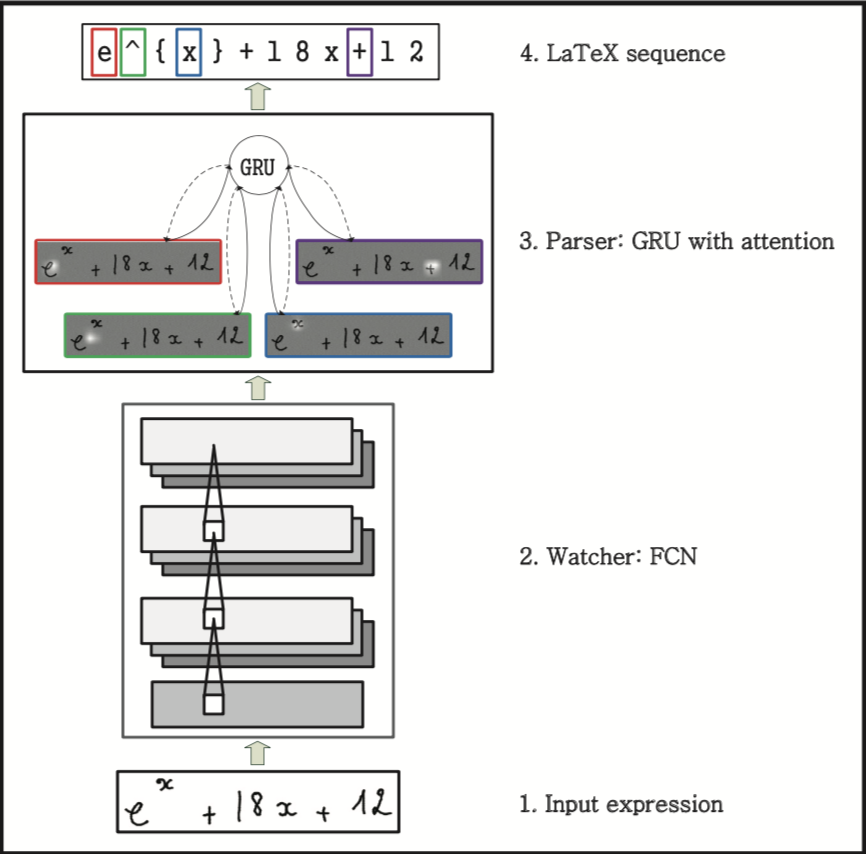
\includegraphics[width=0.6\linewidth]{WAP}
		\vspace{0.5cm}
		\captionof{figure}{Hình minh hoạ các bước thực hiện của phương pháp Watch, Attend and Parser.}
	\end{center}
	
	%	Khác với những bài báo đi trước sử dụng phương pháp phân vùng hay dựa trên ngữ pháp, bài báo này sử dụng phương pháp mang tên Watch, Attend, Parse dựa trên bài toán chú thích cho ảnh \footnote{Thuật ngữ tiếng anh: Image Captioning}. Hệ thống này là sự kết hợp giữa CNN, RNN và một hệ thống ANN (Cụ thể là GRU\cite{cho2014properties}\footnote{Viết tắt: Gated recurrent unit}), CNN đặc trưng cho Watcher sẽ trích đặc trưng ảnh, ANN đặc trưng cho Attend mang nhiệm vụ điều hướng cho mạng biết được vị trí nào sẽ tập trung vào và RNN đặc trưng cho Parser mang nhiệm vụ sinh ra chuỗi Latex chính là đầu ra của hệ thống\\
	%	
	%	Cấu trúc mạng này được chia thành ba phần:
	%	\subsubsection{Watcher}
	%	Bộ phận này có bản chất là một hệ thống mạng nơ-ron tích chập đầy đủ (FCN)\footnote{Thuật ngữ tiếng anh: Fully Convolution Network} có cấu tạo là các lớp tích chập và các lớp pooling xếp chồng lên nhau. Bộ phận này nhận đầu vào là ảnh cần nhận diện và đầu ra là các vector đặc trưng ứng với mỗi pixel của ảnh.
	%	
	%	\subsubsection{Attend}
	%	Bộ phận này hoạt động giống như một hệ thống tổng hợp thông tin, nó có chức năng lấy dữ liệu ký tự vừa được dự đoán từ Parser (sẽ được giải thích bên dưới), từ các vector đặc trưng đã có được từ Watcher và ghi nhận các vị trí đã được xử lý trong ảnh, từ đó dự đoán vị trí tiếp theo để xử lý.
	%	
	%	\subsubsection{Parser}
	%	Bản chất của bộ phận này là một mạng GRU\cite{cho2014properties} nhận dữ liệu đầu vào từ hai bộ phận còn lại, từ đó sinh ra chuỗi Latex
	
	\subsubsection{Context-aware Recognition\cite{context}}
	\label{subsec: context}
	Nhận thấy nhược điểm của phương pháp nhận dạng theo hướng tuần tự là thực hiện hai quá trình nhận dạng ký tự và phân tích cấu trúc một cách độc lập, do đó thông tin cấu trúc của biểu thức không được đưa vào quá trình nhận dạng. Như vậy sẽ dẫn đến việc lỗi tích luỹ qua từng giai đoạn\cite{context}.
	WenHao He cùng các cộng sự của ông đã đề xuất một phương pháp dựa trên CNN, kết hợp với cách học đa nhiệm vụ\footnote{Thuật ngữ tiếng Anh: Multi-task learning}, cố gắng kết hợp hai giai đoạn chuẩn của quá trình nhận dạng biểu thức toán lại với nhau.
	
	Phương pháp mà các ông đưa ra đảm bảo thông tin cấu trúc của biểu thức được đưa vào quá trình nhận dạng và thể hiện trong các ma trận đặc trưng\footnote{Thuật ngữ tiếng Anh: Feature map}\cite{yanlecun}. \\
	Đối với các phương pháp trước, biểu thức phải được phân tách thành những ký hiệu rồi từng ký hiệu này mới được đưa qua bộ nhận dạng. Một số phương pháp phân tách ký hiệu thường được sử dụng như: phân tích thành phần liên thông\footnote{Thuật ngữ tiếng Anh: Connected components}, cắt dựa trên các phép chiếu\footnote{Thuật ngữ tiếng Anh: Projection cutting}\cite{segment}. Tuy nhiên với phương pháp mới này, cả ảnh của biểu thức toán học được đưa qua bộ nhận dạng, chính vì vậy mà thông tin cấu trúc của biểu thức được bảo toàn. \\
	%\vspace{5cm}
	
	Dưới đây là mô hình học của phương pháp này:\\
	
	\begin{figure}[!h]
		\centering
		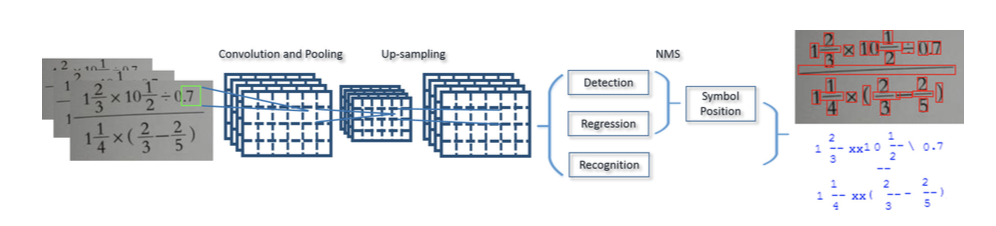
\includegraphics[width=0.9\linewidth]{context_aware.png}
		\vspace{0.2cm}
		\caption{Mô hình học được đề xuất \cite{context}.}
		
	\end{figure}
	
	Ảnh đầu vào sẽ qua một số lớp tích chập, down-sampling và up-sampling để tạo ra một feature map. Feature map này sẽ được gửi đến ba nhiệm vụ, mỗi nhiệm sẽ tạo ra 1 feature map có cùng kích thước với feature map đầu vào. Kiến trúc mạng của 3 nhiệm vụ này là sự kết hợp của các module inception\cite{context}. \\
	Giả sử một điểm $i$ được cho đặt tại toạ độ ($w_i$, $h_i$) của feature map được tạo ra bởi các nhiệm vụ. 
	\begin{itemize}
		\item \textbf{Nhiệm vụ phát hiện} (Dectection task) sẽ cho ra một con số $s$ thể hiện độ tin cậy rằng một ký hiệu được đặt tại $i$.
		\item \textbf{Nhiệm vụ hồi quy} (Regression task) cho ra một vec-tor 4 chiều {$x_1$, $y_1$, $x_2$, $y_2$} thể hiện thông tin về bounding box của ký hiệu được đặt tại $i$.
		\item\textbf{Nhiệm vụ nhận dạng} (Recognition task) gán nhãn cho ký hiệu đặt tại $i$ cùng với xác suất của nhãn đó. 
	\end{itemize}
	
	Như vậy nhiệm vụ phát hiện và hồi quy được thiết kế để định vị trí của ký hiệu trong biểu thức toán học, nhiệm vụ nhận dạng quyết định xem đó là ký hiệu gì.
	
	Phương pháp nhận dạng như trên có thể giải quyết cả những trường hợp là thách thức đối với các phương pháp phân tách và nhận dạng ký hiệu trước đây, cụ thể đó là vấn đề gom nhóm ký hiệu đối với các ký hiệu nhiều phần nhỏ, tách những ký hiệu bị dính nhau.
	
	\subsubsection{QAK\cite{qak}}
	QAK là tên dự án được thực hiện bởi nhóm sinh viên khoá 2011 cũng về đề tài nhận dạng biểu thức toán học.
	
	Phương pháp nhóm sinh viên này xây dựng dựa trên nghiên cứu chính từ hai công trình của Aderson\cite{anderson} và Zanibbi\cite{zanibbi}. Do đó, qua trình nhận dạng biểu thức toán học vẫn đi theo 2 bước chuẩn đó là phân tách ký hiệu và phân tích cấu trúc như đã trình bày ở mục \ref{subsec: context}. 
	
	Dưới đây là mô hình phương pháp mà nhóm đã đề xuất:
	%\vspace{3cm}
	
	\begin{figure}[!h]
		\centering
		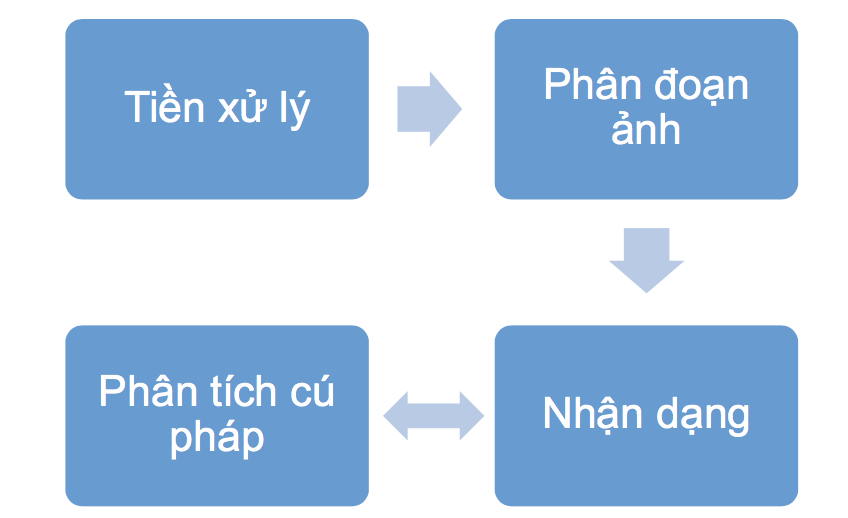
\includegraphics[width=0.5\linewidth]{2011.png}
		\vspace{1cm}
		\caption{Quy trình nhận dạng.}
		
	\end{figure}
	
	\begin{itemize}
		\item Trong bước tiền xử lý, nhóm áp dụng một số kỹ thuật trong xử lý ảnh như: loại nhiễu, ảnh nhị phân,... để tăng cường chất lượng ảnh, hỗ trợ cho bước phân đoạn.
		\item Trong bước phân đoạn ảnh, nhóm dùng kỹ thuật chính là cắt theo hình chiếu\cite{segment} và phân tích thành phần liên thông\cite{segment} cho toán tử lấy căn. Mục tiêu của giai đoạn này là phân tách ảnh chứa biểu thức toán học ban đầu ra thành các mảnh ảnh, mỗi mảnh chỉ chứa 1 ký hiệu toán học. Ngoài ra, ở bước này một cấu trúc cây được xây dựng lưu thông tin của các mảnh ảnh, hỗ trợ cho quá trình phân tích ngữ pháp sau này.
		\item Ở bước nhận dạng, nhóm sinh viên khoá 2011 đã sử dụng một kiến trúc mạng tương tự Lenet-5\cite{yanlecun}.
		\item Với phân tích cú pháp, nhóm sử dụng tập luật \textbf{văn phạm phi ngữ cảnh} \footnote{Thuật ngữ tiếng Anh: Context-free grammar} do chính nhóm đề xuất để giới hạn kết quả đầu ra của quá trình nhận dạng, từ đó tăng khả năng nhận dạng đúng biểu thức. 
	\end{itemize}
	
	%%%%%%%%%%%%%%%%%%%%%%%%%%%%%%%%%%%%%%%%%
	%%%%%%%%%%%%%%%%%%%%%%%%%%%%%%%%%%%%%%%%%
	
	\newpage
	\section{Mô hình đề xuất}
	\label{sec: mohinhdexuat}
	\subsection{Tổng quan}
	Nhóm chọn hướng tiếp cận là thực hiện tuần tự hai quá trình nhận dạng ký tự và phân tích cấu trúc để giải quyết đề tài. Quy trình thực hiện như hình bên dưới.
	\begin{center}
		
		\centering
		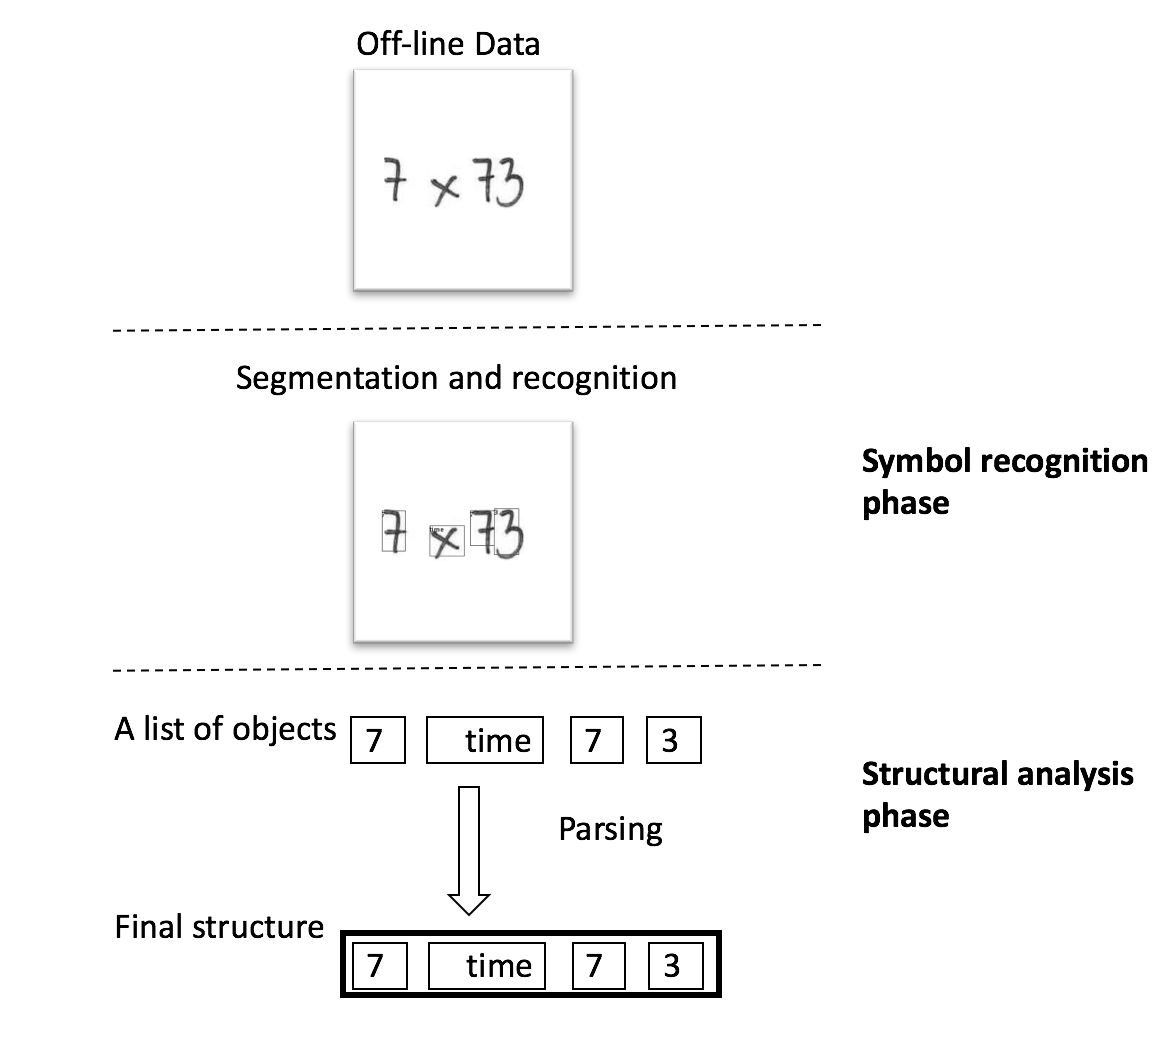
\includegraphics[width=0.8\linewidth]{overview}
		\vspace{0.5cm}
		\captionof{figure}{Mô hình phương pháp.}
	\end{center}
	\begin{itemize}
		\item Ở bước nhận dạng ký tự, ảnh đầu vào là ảnh xám sẽ qua mạng SSD\cite{liu2016ssd} để tạo ra một danh sách các nhãn và bounding box được kỳ vọng là tương ứng với các ký tự có trong ảnh.
		\item Với giai đoạn phân tích cấu trúc, từ danh sách nhãn và bounding box trả ra từ giai đoạn trước, sử dụng bộ phân tích cấu trúc DRACULAE \cite{zanibbi} để sinh ra chuỗi Latex.
	\end{itemize}
	Việc lựa chọn SSD cho giai đoạn nhận dạng ký tự là để khắc phục hạn chế của cách tiếp cận tuần tự khi thông tin cấu trúc ảnh vẫn được lưu giữ qua thông tin các bounding box của ký tự. 
	\subsection{Giai đoạn nhận diện ký tự}
	
	\subsubsection{Mạng cơ sở}
	
	Về cấu trúc của SSD\cite{liu2016ssd}, nhóm đã sử dụng mạng VGG16\cite{simonyan2014very} cho phần mạng cơ sở. Cấu trúc của mạng VGG16\cite{simonyan2014very} gồm tổ hợp các lớp tích chập và lớp pooling xếp chồng lên nhau, ở cuối mạng có các lớp liên kết đầy đủ \footnote{Thuật ngữ tiếng Anh: Fully connected layer} để giảm kích thước tensor và cuối cùng là xuất ra vector có số chiều phù hợp (có số chiều bằng với số lớp đối tượng cần dự đoán).
	
	\begin{center}
		
		\centering
		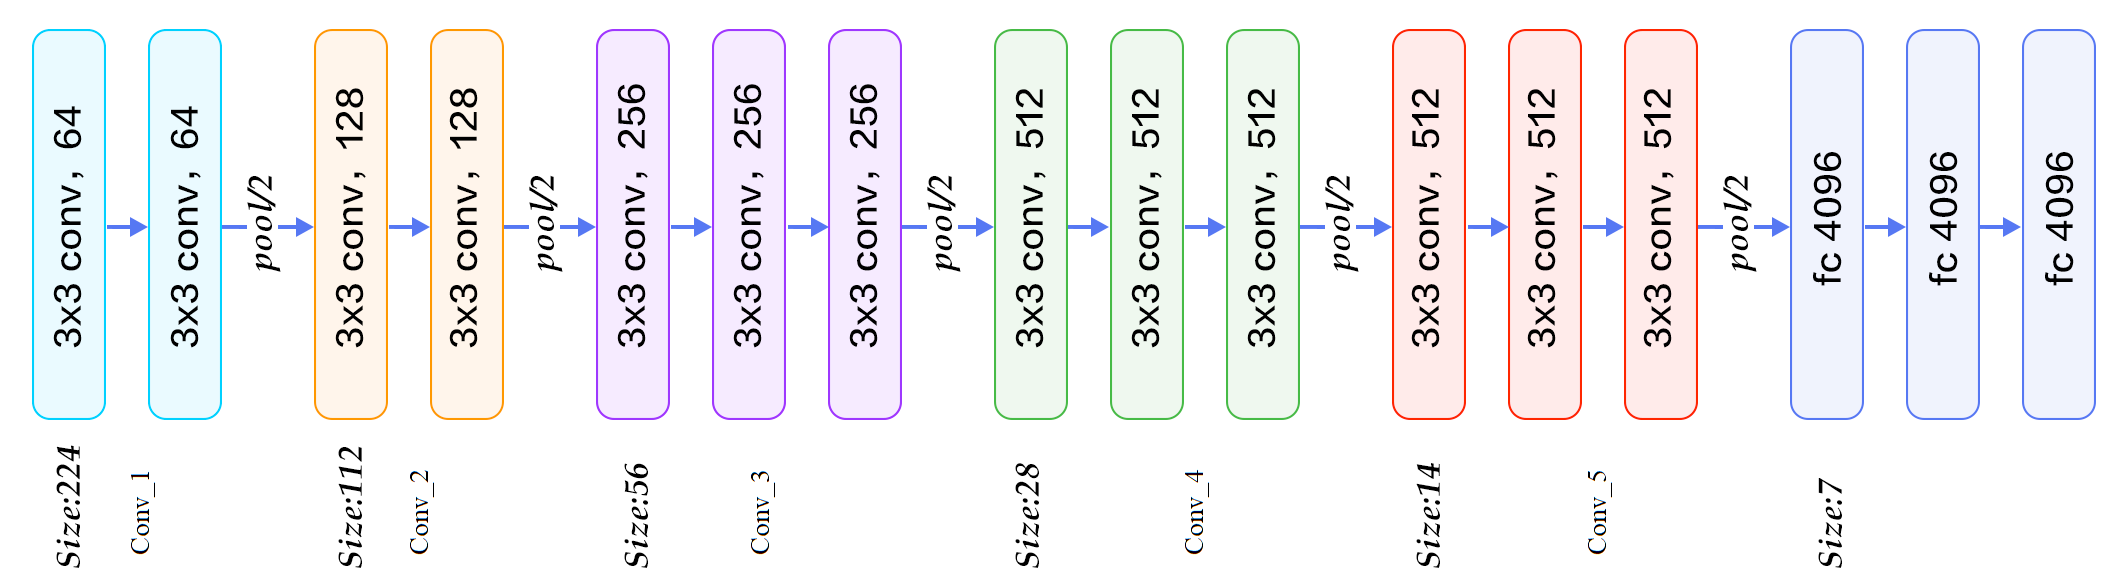
\includegraphics[width=0.8\linewidth]{vgg16.png}
		\vspace{0.5cm}
		\captionof{figure}{Cấu tạo mạng VGG16\cite{simonyan2014very}}
	\end{center}
	
	Như hình vẽ bên trên, các lớp tích chập và lớp pooling được gom lại thành các cụm, sau hai đến ba lớp tích chập là một lớp pooling. Số kênh của tensor chạy trong mạng được nâng dần từ 64 lên 512 về phía cuối mạng. Khi đưa mạng cơ sở vào mạng SSD\cite{liu2016ssd}, các lớp liên kết đầy đủ sẽ được bỏ đi và bộ phận phân loại sẽ được chèn vào vị trí tương ứng. Khi đó, ta cần phải chuyển model của mạng VGG\cite{simonyan2014very} sang mạng SSD\cite{liu2016ssd}.
	
	\subsubsection{Thân mạng SSD\cite{liu2016ssd}}
	\label{sec: thanSSD}
	Sau khi ảnh đi qua mạng cơ sở và sinh ra một feature map, dữ liệu này sẽ tiếp tục đi qua các lớp tích chập và pooling kết hợp với việc trích ra feature map ở một số vị trí nhất định để đưa vào lớp multibox,  Mô hình cụ thể của phần thân mạng SSD\cite{liu2016ssd} nhóm để xuất được thể hiện ở ảnh dưới.
	
	\begin{center}
		
		\centering
		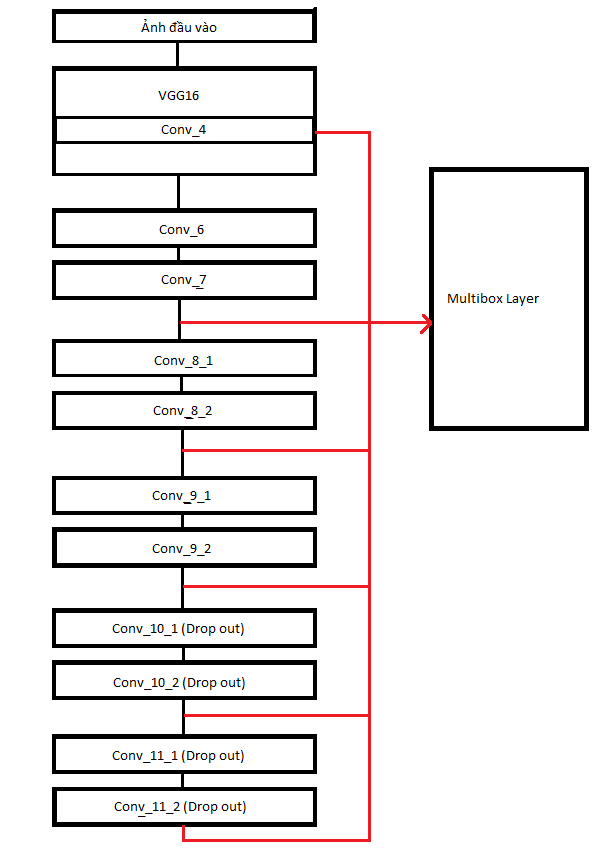
\includegraphics[width=0.8\linewidth]{SSD_Layers.png}
		\vspace{0.5cm}
		\captionof{figure}{Sơ đồ các lớp trong mạng SSD\cite{liu2016ssd}}
	\end{center}
	
	Trong đó Khối VGG166 là phần mạng VGG16\cite{simonyan2014very} đã được lược bỏ các lớp liên kết đầy đủ, khối Conv\_4 nằm trong khối VGG16 này do Conv\_4 trong ảnh là lớp tích chập thứ 10 trong mạng VGG\cite{simonyan2014very}. Các khối còn lại được thể hiện trong bảng sau:
	
	\begin{center}
		\begin{tabular}{||c | c | c | c | c | c ||} 
			\hline
			Khối & \makecell{ Số kênh \\ đầu vào } & \makecell{ Số kênh \\ đầu ra} & Kích thước nhân &  \makecell{ Chèn thêm \\ (Padding) } &  \makecell{ Bước \\ (Stride) } \\ [0.5ex] 
			\hline\hline
			Conv\_6 & 512 & 1024 & 3 & 1 & 1 \\ 
			\hline
			Conv\_7 & 1024 & 1024 & 3 & 6 & 1 \\ 
			\hline
			Conv\_8\_1 & 1024 & 256 & 1 & 0 & 1 \\ 
			\hline
			Conv\_8\_2 & 256 & 512 & 3 & 1 & 2 \\ 
			\hline
			Conv\_9\_1 & 512 & 128 & 1 & 0 & 1 \\ 
			\hline
			Conv\_9\_2 & 128 & 256 & 3 & 1 & 2 \\ 
			\hline
			Conv\_10\_1 & 256 & 128 & 1 & 0 & 1 \\ 
			\hline
			Conv\_10\_2 & 128 & 256 & 3 & 1 & 2 \\ 
			\hline
			Conv\_11\_1 & 256 & 128 & 1 & 0 & 1 \\ 
			\hline
			Conv\_11\_2 & 128 & 256 & 3 & 0 & 1 \\ 
			\hline
		\end{tabular}
		\captionof{table}{Cấu hình các lớp tích chập trong mạng SSD300\cite{liu2016ssd}}
	\end{center}
	
	
	Các lớp tích chập đều sử dụng hàm truyền là hàm ReLu\cite{relu}. Ở sau các lớp Conv\_10\_1, Conv\_10\_2, Conv\_11\_1, Conv\_11\_2 thì có thêm một lớp dropout\cite{srivastava2014dropout} với hệ số dropout là 0.2. Giữa một số lớp tích chập và pooling là nơi các feature map được trích ra để thực hiện công đoạn phát hiện, phân loại ký tự (được thể hiện bởi các mủi tên màu đỏ trên hình), cụ thể:
	
	\begin{itemize}
		\item Ngay sau khối tích chập - pooling 512 thứ nhất trong mạng VGG\cite{simonyan2014very} (hay sau lớp pooling của lớp tích chập thứ 10 của mạng VGG\cite{simonyan2014very} - hay Conv\_4).
		\item Sau các khối tích chập Conv\_7, Conv\_8, Conv\_9, Conv\_10, Conv\_11.
	\end{itemize}
	
	Đối với mạng SSD300\cite{liu2016ssd}, kích thước của các feature map ứng với số dự đoán được thể hiện ở bảng sau:
	
	\begin{center}
		\begin{tabular}{||c | c | c | c ||} 
			\hline
			\makecell{ Feature map \\ Sinh bởi } & \makecell{ Kích thước} & \makecell{Aspect Ratio } &  \makecell{ Số dự đoán } \\ [0.5ex] 
			\hline\hline
			Conv\_4 & $512 \times 38 \times 38$ & $ \{ 1, \frac{1}{2} , 2\} $ & 5776 \\ 
			\hline
			Conv\_7 & $1024 \times 19 \times 19$ & $ \{ 1, \frac{1}{2} , 2, \frac{1}{3}, 3\} $ & 2166 \\ 
			\hline
			Conv\_8 & $512 \times 10 \times 10$ &  $ \{ 1, \frac{1}{2} , 2, \frac{1}{3}, 3\} $ & 600 \\ 
			\hline
			Conv\_9 & $256 \times 5 \times 5 $ &  $ \{ 1, \frac{1}{2} , 2, \frac{1}{3}, 3\} $ & 150  \\ 
			\hline
			Conv\_10 & $256 \times 3 \times 3$ & $ \{ 1, \frac{1}{2} , 2\} $ & 36 \\ 
			\hline
			Conv\_11 & $256 \times 1 \times 1$ & $ \{ 1, \frac{1}{2} , 2\} $ & 4 \\ 
			\hline
		\end{tabular}
		\captionof{table}{Thông tin của các feature map trích được từ mạng SSD300\cite{liu2016ssd}}
	\end{center}
	
	Như vậy, ứng với mỗi ảnh, hệ thống sinh ra 8732 dự đoán. Tương ứng, bộ phận mã hóa của mạng SSD300\cite{liu2016ssd} cũng có những thông số:
	
	\begin{itemize}
		\item Danh sách kích thước feature map: (38, 19, 10, 5, 3, 1)
		\item Danh sách kích thước các ổ chuẩn (với $s_0 = 0.1$, $s_{min} = 0.2$ và $s_{max} = 0.9$): (30, 60, 111, 162, 213, 264, 315)
		\item Ngưỡng Jaccard\cite{Jaccard}: 0.5.
	\end{itemize}
	
	
	\newpage
	\subsection{Giai đoạn phân tích cú pháp}
	
	Nhóm sử dụng phương pháp phân tích cú pháp DRACULAE được giới thiệu trong \cite{zanibbi}. Bộ phân tích cú pháp DRACULAE\cite{zanibbi} này có nhiệm vụ chuyển dữ liệu dự đoán là các bounding box và nhãn của ký tự sang dữ liệu biểu thức toán học dạng Latex. Trong quá trình phân tích cú pháp, biểu thức được lưu trữ dưới dạng cây  BST\cite{zanibbi} là một cấu trúc cây dựa trên các đường cơ sở, các nhánh của cây thể hiện một phân vùng bên trên, bên dưới, ... của nút và là một phân vùng ảnh có đường cơ sở riêng và Lexed - BST\cite{zanibbi} là một cấu trúc cây tương tự như BST nhưng thay vì chỉ biểu thị vị trí bên trên, bên dưới thì cây biểu thị quan hệ phân số, chỉ số trên, chỉ số dưới, ...\\
	
	\begin{center}
		\centering
		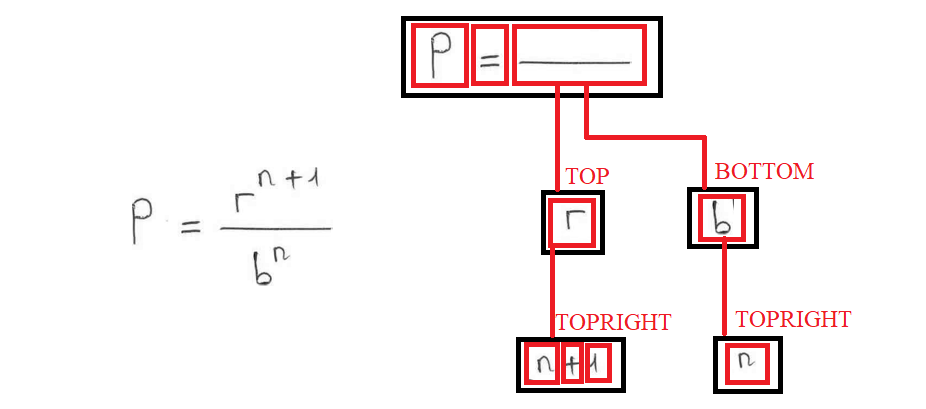
\includegraphics[width=0.95\linewidth]{BST.png}
		\vspace{0.5cm}
		\captionof{figure}{Một cây BST\cite{zanibbi} (Các đường màu đỏ biểu thị mối quan hệ nút cha con)}
	\end{center}	
	
	\begin{center}
		\centering
		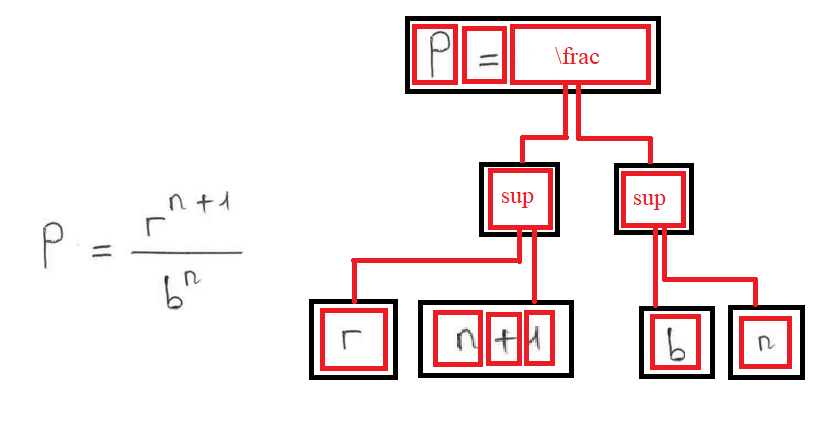
\includegraphics[width=0.85\linewidth]{lexBST.png}
		\vspace{0.5cm}
		\captionof{figure}{Một cây Lexed - BST\cite{zanibbi}}
	\end{center}
	
	
	
	\subsubsection{Sinh cây BST\cite{zanibbi}}
	
	Đây là giai đoạn phức tạp nhất và cũng là quan trọng nhất, ở giai đoạn này, dữ liệu đầu ra từ mạng SSD\cite{liu2016ssd} là danh sách các bounding box sẽ được phân tích và xây dựng một cây BST\cite{zanibbi}. Công việc này có thể được phân ra thành bốn công đoạn: Tìm ký tự chủ đạo\cite{zanibbi}\footnote{Thuật ngữ tiếng Anh: Dominate symbol.}, xác định những ký tự trên đường cơ sở, tái phân vùng và xử lý nút con.\\
	
	Trước khi tiến hành sinh cây, ta cần phải phân loại các ký tự vào những thể loại khác nhau. Theo Zanibbi đã đề xuất cho DRACUALE\cite{zanibbi}, các ký tự được phân vào các lớp như bảng dưới:
	
	\begin{center}
		\begin{tabular}{||c | c | c c c c ||} 
			\hline
			Lớp ký tự & Tung độ trọng tâm & Bên dưới & Bên trên & Chỉ số dưới & Chỉ số trên \\ [0.5ex] 
			\hline\hline
			\makecell{Non-Script \\ Các ký tự phép tính\\ $(+, -, \rightarrow, ... )$} & $\frac{1}{2}H$ & $\frac{1}{2}H$ & $\frac{1}{2}H$ & - & - \\ 
			\hline
			\makecell{Open Bracket \\ Ký tự mở ngoặc \\ ( } & $cH$ & $min(Y)$ & $max(Y)$ & - & - \\
			\hline
			\makecell{Root \\ Ký tự căn \\ $\sqrt{}$ } & $cH$ & $min(Y)$ & $max(Y)$ & $tH$ & $H - tH$ \\
			\hline
			\makecell{Variable Range \\ Ký tự có thể viết \\ ở trên hoặc dưới \\ $\sum$, $\int$, $\lim$ ... } & $\frac{1}{2}H$ & $tH$ & $H-tH$ & $tH$ & $H- tH$ \\
			\hline
			\makecell{Ascender \\ Ký tự nổi lên \\ A..Z, 0..9, b,d,f ... } & $cH$ &  $tH$ & $H-tH$ & $tH$ & $H- tH$ \\
			\hline
			\makecell{Descender \\ Ký tự chìm xuống \\ g, p, y, j, ..., b,d,f ... } & $H - cH$ &  $\frac{1}{2}H + t\frac{1}{2}H$ & $H-t\frac{1}{2}H$ & $\frac{1}{2}H + t\frac{1}{2}H$ & $H-t\frac{1}{2}H$ \\ 
			\hline
			\makecell{Centered \\ Ký tự trung tâm \\ o, n, u, \}, ) ... } & $\frac{1}{2}H$ &  $tH$ & $H-tH$ & $tH$ & $H- tH$
			\\ \hline
			
			
		\end{tabular}
		\captionof{table}{Bảng phân lớp các ký tự cần nhận diện và các ngưỡng xác định phân vùng con}
		
	\end{center}
	
	Trong đó:
	\begin{itemize}
		\item Các cột thứ hai trở đi là tọa độ của một số điểm, ngưỡng đặc biệt tính từ góc trái bên dưới của ký tự. Cột "Tung độ trọng tâm" thể hiện tung độ y của trọng tâm của ký tự, cột "bên dưới" và "bên trên" thể hiện ngưỡng trên và ngưỡng dưới của ký tự, các ký tự vượt ngoài ngưỡng đó sẽ được xem là nằm bên trên hoặc nằm bên dưới ký tự đang xét. Cột chỉ số trên, chỉ số dưới thể hiện ngưỡng để được phân vào vùng chỉ số trên, chỉ sô dưới. Một ký tự nằm trong khoảng chỉ số dưới đến chỉ số trên của một ký tự khác thì hai ký tự xem là liền kề nhau. Riêng hai lớp Non-scipt và Open Bracket có giá trị hai cột này không xác định là do những ký tự của lớp này không có chỉ số trên, dưới.
		\item $H$ là chiều cao của ký tự.
		\item $c$ (Viết tăt của centroid ratio): là tham số để xác định trọng tâm cho một số ký tự đặc biệt (ví dụ như các ký tự ngoặc hoặc chìm xuống dưới), tùy người viết chữ có thể có những giá trị phù hợp khác nhau.
		\item $t$ Là tham số ảnh hưởng đến ngưỡng cho chỉ số trên, dưới và chỉ phần bên trên, bên dưới. Tham số này biểu thị sự nhạy cảm đối với những ký tự trên dưới.
	\end{itemize}
	
	
	Trước khi tiến hành sinh cây BST, danh sách bounding box cần phải được sắp xếp theo chiều tăng dần hoành độ của mép phải bounding box $x$ (hay cụ thể hơn là $min(x)$). \\
	
	\subsubsection*{Tìm ký tự chủ đạo\cite{zanibbi}}
	
	Trong hầu hết trường hợp, ký tự chủ đạo\cite{zanibbi} là ký tự nằm bên trái nhất, tuy vậy, ta vẫn cần phải kháng được những trường hợp người dùng viết chữ không chuẩn gây thụt ra ngoài, hoặc những ký tự có dạng như:
	
	$$ \sum^{n = 100000} a $$
	Thì ký tự chủ đạo\cite{zanibbi} là $\sum$ nhưng ký tự bên trái nhất lại là $n$, DRACULAE\cite{zanibbi} được thiết kế để có thể chống lại những trường hợp như vậy.\\
	
	Để tìm ký tự chủ đạo\cite{zanibbi}, ta tìm ký tự bên trái nhất dựa trên 3 điều kiện:
	
	\begin{itemize}
		\item Không bị thống trị bởi ký tự phân số. Kiểm tra bằng cách tìm kiếm một ký tự dấu gạch ngang trong vùng ảnh phía trên, phía dưới.
		\item Không bị bọc bởi ký tự căn ($\sqrt{}$).
		\item Nếu ký tự đang xét thuộc lớp Variable Range thì không được phép có ký tự liền kề bên trái.
	\end{itemize}
	
	%Để tìm ký tự chủ đạo\cite{zanibbi}, ta cần thực hiện theo những công đoạn sau:
	%\begin{itemize}
	%	\item Trước hết, ta tìm ký tự nằm bên trái nhất.
	%	\item Kiếm tra ký tự đó có phải là Variable Range. Nếu đúng thì ta kiểm tra xem ký tự đó có bị thống trị bởi một phân số hay không, nếu có thì ký tự chủ đạo\cite{zanibbi} là ký tự phân số, nếu không thì ký tự chủ đạo\cite{zanibbi} là ký tự Variable Range vừa tìm được. Nếu ký tự vừa tìm được không phải là Variable Range, thì ta tìm kiếm ký tự Variable Range nằm bên trái nhất và sang bước tiếp theo.
	
	%	\item Nếu không còn ký tự Variable Range nào khác, thì ký tự bên trái nhất vừa tìm được ở bước trên được kiểm tra bị thống trị bởi phân số hay không và trả về ký tự chủ đạo\cite{zanibbi} (ký tự đó hoặc ký tự phân số). Nếu còn một ký tự Variable Range khác trong biểu thức, ta tiếp tục với bước kế tiếp.
	
	%	\item Ta kiểm tra xem ký tự Variable Range khác đó có ký tự nào nằm liền kề bên trái không. Nếu không thì tự Variable Range được kiểm tra xem có bị thống trị bởi ký tự phân số hay không và chọn ký tự chủ đạo\cite{zanibbi} ký tự phù hợp. Nếu tồn tại ký tự liền kề bên trái, thì ký tự bên trái nhất được kiểm tra có bị thống trị bởi phân số không và chọn ký tự chủ đạo\cite{zanibbi} phù hợp.
	
	%\end{itemize}
	
	\subsubsection*{Xác định ký tự trên đường cơ sở}
	
	Sau khi đã có được ký tự chủ đạo\cite{zanibbi}, ta cần phải tìm những ký tự liền kề theo chiều ngang với ký tự vừa tìm được, những ký tự này chính là ký tự trên đường cơ sở. Để xác định các ký tự trên đường cơ sở, ta lấy ký tự chủ đạo\cite{zanibbi} vừa xác định được để xét:
	
	\begin{enumerate}
		\item Ta phần vùng các ký tự nằm ở vùng bên trên, bên dưới, góc trên bên trái và góc dưới bên trái (không phân vùng các ký tự nằm bên phải) vào nút con của nút đang xét.
		\item Nếu như ký tự đang xét thuộc lớp Non-script, ký tự đó được đánh dấu nằm trên đường chủ đạo\cite{zanibbi}, ta quay lại tìm ký tự chủ đạo\cite{zanibbi} trong các ký tự còn lại và xác định các ký tự trên đường cơ sở với ký tự chủ đạo\cite{zanibbi} đó.
		\item Ta kiểm tra danh sách các ký tự còn lại xem có ký tự nào liền kề bên phải với ký tự đang xét hay không, nếu có, ta kiểm tra ký tự đó có bị thống trị bởi ký tự khác hay không và quay lại bước 1 với ký tự được xét là ký tự thống trị nhất (hoặc chính ký tự liền kề nhất vừa tìm được đối với trường hợp nó không bị thống trị bởi ký tự nào).
		\item Nếu hệ thống chạy đến bước này thì có nghĩa là trong các ký tự còn lại, không còn ký tự nào liền kề với ký tự đang xét, vì vậy ta tiến hành phân vùng đưa các ký tự còn lại vào nút con góc trên bên phải (chỉ số trên) và góc dưới bên phải (chỉ số dưới) của nút đang xét.
	\end{enumerate}
	
	Sau khi thực hiện bước này lần đầu tiên, ta thu được một cây có ba tầng, tầng đầu chứa nút gốc, tầng thứ hai chứa các ký tự nằm trên đường cơ sở, tầng thứ ba chứa các nút con của các nút chứa ký tự nằm trên đường cơ sở, các nút con này có thể chứa một hoặc nhiều ký tự, chưa là một cây.
	
	\subsubsection*{Tái phân vùng}
	Ở bước trước, nút con được phân vào vùng góc trên bên trái và góc dưới bên trái, điều này không có ý nghĩa đối với ngữ nghĩa của biểu thức toán học và khó khăn trong việc sinh cây Lexed BST\cite{zanibbi} sau này. Vì vậy ở bước này, các nút con sẽ được thay đổi vị trí cho phù hợp với ngữ nghĩa của biểu thức. Cụ thể:
	
	\begin{itemize}
		\item Các nút con thuộc vùng góc trên bên trái và góc dưới bên trái sẽ được phân vùng vào vùng góc trên bên phải và góc dưới bên phải của ký tự trước đó.
		\item Riêng đối với các ký tự Variable Range, hệ thống thực hiện thêm bước kiểm tra sự liền kề đối với những ký tự trong vùng con để phân vùng phù hợp.
	\end{itemize}
	
	\iffalse
	, chương trình sẽ kiểm tra từng cặp ký tự liền kề theo thứ tự từ trái sang phải, ta gọi ký tự bên trái là $A$ và ký tự bên phải là $B$:\\
	
	\begin{itemize}
		\item Nếu $B$ không thuộc lớp Variable Range, và $B$ không có nút con ở vùng bên trên, ta gắn nút góc trên bên trái của ký tự $B$ vào nút góc trên bên phải (chỉ số trên) của $A$. 
		\item Nếu $B$ thuộc lớp Variable Range thì ta sẽ phân vùng những ký tự liền kề với ký tự đầu tiên trong nút con góc trên bên trái của $B$ vào vùng bên trên của $B$. 
		\item Nếu $A$ thuộc lớp Variable Range thì ta phải tiến hành gộp các vùng góc trên bên trái, bên trên và góc trên bên phải thành một vùng bên trên duy nhất.
	\end{itemize}
	
	Với một số biểu thức đặc biệt hoặc nhập nhằng thì việc phân vùng sẽ không chính xác, để khắc phục điều này, ta cần phải có thêm công đoạn hậu xử lý.\\
	
	\fi
	
	\subsubsection*{Xử lý nút con}
	
	Tới bước này, ta đã có một cây có ba tầng với tầng thứ hai có phân vùng nút con khá chuẩn xác. Nhiệm vụ bây giờ là phải tiếp tục phân vùng cho các nút con của các ký tự trên đường cơ sở. Việc này được thực hiện bằng cách xem từng nút con là từng vùng ảnh mới riêng biệt và thực hiện lại ba bước trên để thu được các cây con. \\
	
	Sau quá trình này, ta thu được một cây BST biểu thị vị trí tương đối giữa các nút. Cây này tiếp tục được đi qua [Lexical Pass] để thu được Lexed - BST\cite{zanibbi}.
	
	\subsubsection{Sinh cây Lexed - BST\cite{zanibbi}}
	
	Sau khi đã thu được cây BST từ danh sách các bounding box, nhiệm vụ còn lại là không quá phức tạp. Trước khi tạo được chuỗi Latex, ta cần phải sinh ra được một cây Lexed - BST\cite{zanibbi}, cây này chứa các thông tin như "nhóm ký tự" và cấu trúc biểu thức:
	
	\begin{itemize}
		\item Nhóm ký tự: Ban đầu, các ký tự được gom thành từng nhóm có nghĩa (Ví dụ các ký tự "s", "i", "n" thì sẽ được gộp lại thành một ký tự "sin" duy nhất.
		\item Ta sử dụng các luật khác nhau để sinh ra cây Lexed - BST\cite{zanibbi}.
	\end{itemize}
	
	\subsubsection*{Luật sinh}
	
	
	Để chuyển từ cây BST\cite{zanibbi} sang cây lexed - BST\cite{zanibbi}, nhóm có đề xuất một số luật sinh: \\
	Gọi ký tự đang xét là $A$
	\begin{itemize}
		\item Nếu cây BST $B$ nằm trong nút con góc phải bên dưới của $A$ thì sinh ra một nút sub(A, B)
		\item Nếu cây BST $B$ nằm trong nút con góc phải bên trên của $A$ thì sinh ra một nút sup(A, B)
		\item Nếu cây BST $B$ nằm trong nút con bên trong của $A$ và $A$ là ký tự căn ($\sqrt{}$) thì sinh ra một nút sqrt(B)
		\item Nếu $A$ có nút con bên trên hoặc bên dưới (hoặc cả hai), thì tùy thuộc vào ký tự $A$ mà ta sinh ra các nút khác nhau (Ví dụ như các ký tự $\sum$, $\lim$, $\prod$ , $\int$, $\rightarrow$ và quan trọng nhất là dấu gạch ngang trong phân số)
		
	\end{itemize}
	
	Sau khi sinh được cây Lexed - BST\cite{zanibbi}, hệ thống sẽ duyệt qua cây theo chiều tiền thứ tự để sinh mã Latex.
	
	%%%%%%%%%%%%%%%%%%%%%%%%%%%%%%%%%%%%%
	%%%%%%%%%%%%%%%%%%%%%%%%%%%%%%%%%%%%%
	\newpage
	\section{Hiện thực, đánh giá}
	
	Để xây dựng hệ thống nhận diện biểu thức toán học viết tay, nhóm cần hoàn thành ba công việc chính bao gồm thu thập dữ liệu, huấn luyện mạng SSD và xây dựng chương trình sinh mã latex.
	
	\subsection{Chuẩn bị dữ liệu}
	Việc chuẩn bị dữ liệu bao gồm xây dựng tập ký tự viết tay thường dùng trong Toán học và xây dựng bộ những ảnh biểu thức Toán học viết tay sử dụng những ký hiệu đó.
	\subsubsection{Xây dựng tập ký tự}
	Như đã đề cập trong chương 1, nhóm kế thừa tập ký hiệu Toán viết tay bao gồm chữ cái, chữ số, các ký hiệu Hy Lạp của nhóm sinh viên khoá 2011\cite{qak}.\\
	Một số thông tin về tập dữ liệu\footnote{Sử dụng thông tin được nêu trong luận văn \cite{qak}.}:
	\begin{itemize}
		\item Số người tham gia: khoảng 20
		\item Số lượng ký hiệu: 46197
		\item Số lượng nhãn: 88
		\item Các nhãn ký hiệu trong tập dữ liệu: 0, 1, 2, 3, 4, 5, 6, 7, 8, 9, a, b, c, d, e, f, g, h, i,
		j, k, l, m, n, o, p, q, r, s, t, u, v, w, x, y, z, A, B, C, D, E, F, G, H, I, J, K, L, M, N, O, P, Q, R, S, T, U, V, W, X, Y, Z, (, ), +, -, *, /, =,  $\textcolor{black}{\int}$, $\textcolor{black}{\alpha}$, $\textcolor{black}{\beta}$, $\textcolor{black}{\gamma}$, $\textcolor{black}{\delta}$, $\textcolor{black}{\epsilon}$, $\textcolor{black}{\theta}$, $\textcolor{black}{\lambda}$, $\textcolor{black}{\mu}$, $\textcolor{black}{\pi}$, $\textcolor{black}{\rho}$, $\textcolor{black}{\sigma}$, $\textcolor{black}{\phi}$, $\textcolor{black}{\omega}$, $\textcolor{black}{\Delta}$, $\textcolor{black}{\Pi}$, $\textcolor{black}{\Sigma}$, $\textcolor{black}{\Phi}$, $\textcolor{black}{\Omega}$.
	\end{itemize}
	Tuy nhiên, nhóm đã bổ sung thêm 18 nhãn ký hiệu vào tập dữ liệu này dựa trên cách thu thập được giới thiệu trong luận văn của nhóm sinh viên khoá 2011\cite{qak}.\\
	Thông tin mô tả tập ký hiệu được sử dụng cho đề tài:
	\begin{itemize}
		\item Số người tham gia: 36
		\item Số lượng ký hiệu: 52353
		\item Số lượng nhãn: 106
		\item Các nhãn ký hiệu trong tập dữ liệu: 0, 1, 2, 3, 4, 5, 6, 7, 8, 9, a, b, c, d, e, f, g, h, i, j, k, l, m, n, o, p, q, r, s, t, u, v, w, x, y, z, A, B, C, D, E, F, G, H, I, J, K, L, M, N, O, P, Q, R, S, T, U, V, W, X, Y, Z, (, ), +, -, *, /, =, $\textcolor{black}{\int}$, $\textcolor{black}{\alpha}$, $\textcolor{black}{\beta}$, $\textcolor{black}{\gamma}$, $\textcolor{black}{\delta}$, $\textcolor{black}{\epsilon}$, $\textcolor{black}{\theta}$, $\textcolor{black}{\lambda}$, $\textcolor{black}{\mu}$, $\textcolor{black}{\pi}$, $\textcolor{black}{\rho}$, $\textcolor{black}{\sigma}$, $\textcolor{black}{\phi}$, $\textcolor{black}{\omega}$, $\textcolor{black}{\Delta}$, $\textcolor{black}{\Pi}$, $\textcolor{black}{\Sigma}$, $\textcolor{black}{\Phi}$, $\textcolor{black}{\Omega}$, $\textcolor{blue}{\sin}$, $\textcolor{blue}{\cos}$, $\textcolor{blue}{\tan}$, $\textcolor{blue}{\log}$, $\textcolor{blue}{\lim}$, $\textcolor{blue}{\surd}$, $\textcolor{blue}{\rightarrow}$, $\textcolor{blue}{\geq}$, $\textcolor{blue}{\leq}$, $\textcolor{blue}{\forall}$, $\textcolor{blue}{\exists}$, $\textcolor{blue}{\in}$, \textcolor{blue}{!}, \textcolor{blue}{.}, $\textcolor{blue}{\ldots}$, $\textcolor{blue}{\div}$, $\textcolor{blue}{\neq}$, $\textcolor{blue}{\infty}$.
		
	\end{itemize}
	\subsubsection{Xây dựng tập biểu thức}
	Để phục vụ quá trình huấn luyện của mạng SSD được nêu trong Chương 4, ngoài tập ký tự nhóm cần phải xây dựng thêm tập ảnh các biểu thức Toán học viết tay.\\
	\subsubsubsection{Quá trình thu thập dữ liệu}
	\begin{itemize}
		\item Tạo biểu mẫu để thu dữ liệu. Biễu mẫu này có 6 hàng và 2 cột như hình bên dưới. 
		\begin{center}
			\centering
			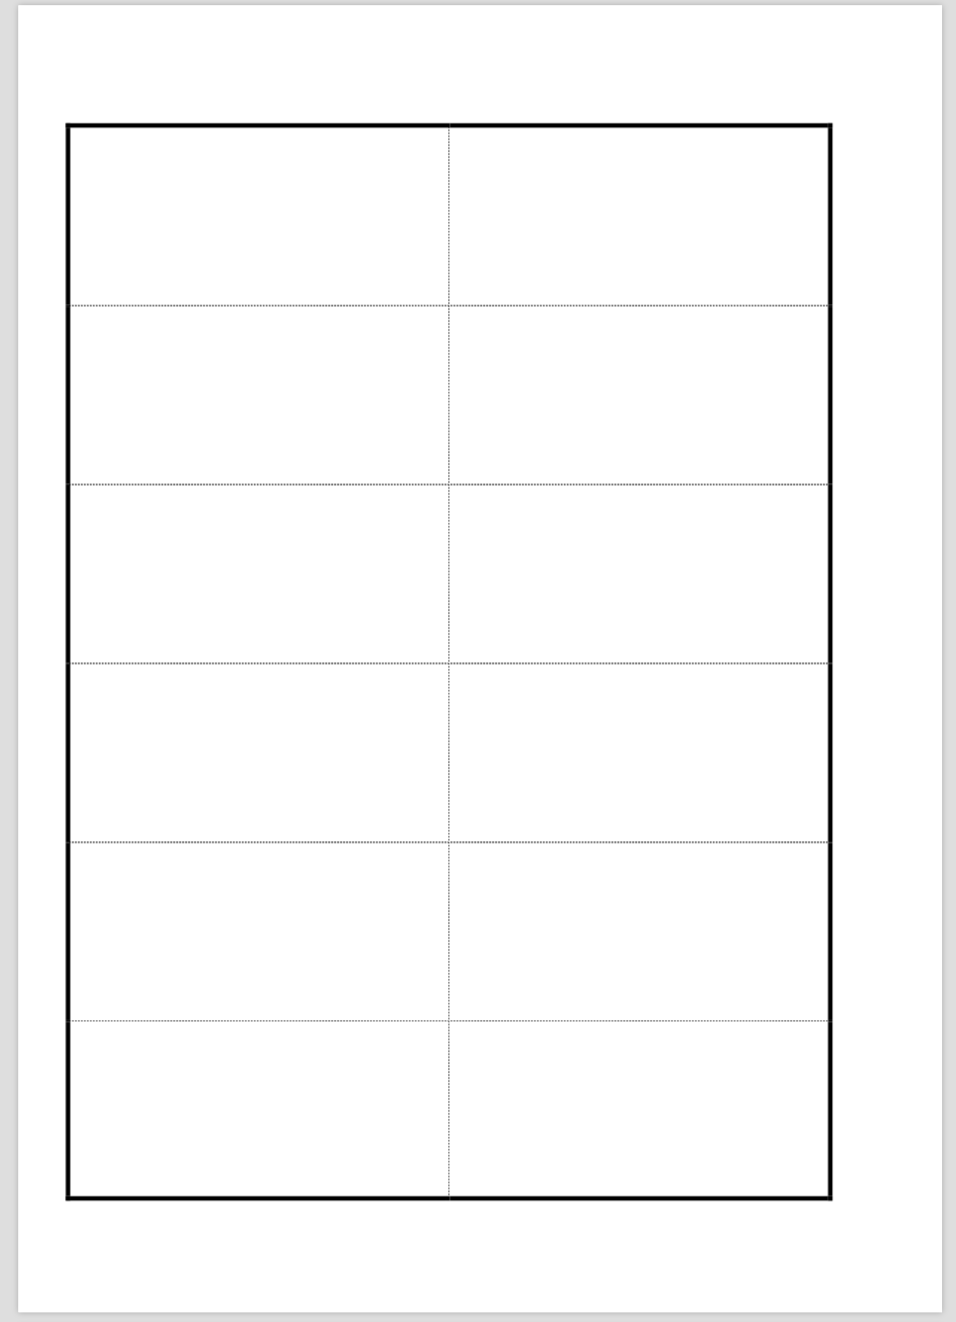
\includegraphics[width=0.8\linewidth]{getExp}
			\vspace{0.5cm}
			\captionof{figure}{Biểu mẫu để thu thập dữ liệu.}
		\end{center}
		\item Chuẩn bị bộ biểu thức làm gợi ý cho người viết. Các biểu thức này được sao chép từ tập dữ liệu CROHME 2014\cite{crohme}. 
		
		\begin{center}
			\centering
			\includegraphics[width=0.9\linewidth]{Exp_sample1}
			\vspace{0.5cm}
			\captionof{figure}{Ví dụ mẫu biểu thức gợi ý cho người viết.}
		\end{center}
		\item Người tham gia viết sẽ nhận được biểu mẫu và công thức gợi ý. Sau đó họ sẽ viết lại những công thức này lên tờ biểu mẫu bằng chính nét chữ thường ngày của họ. 
		\begin{center}
			\centering
			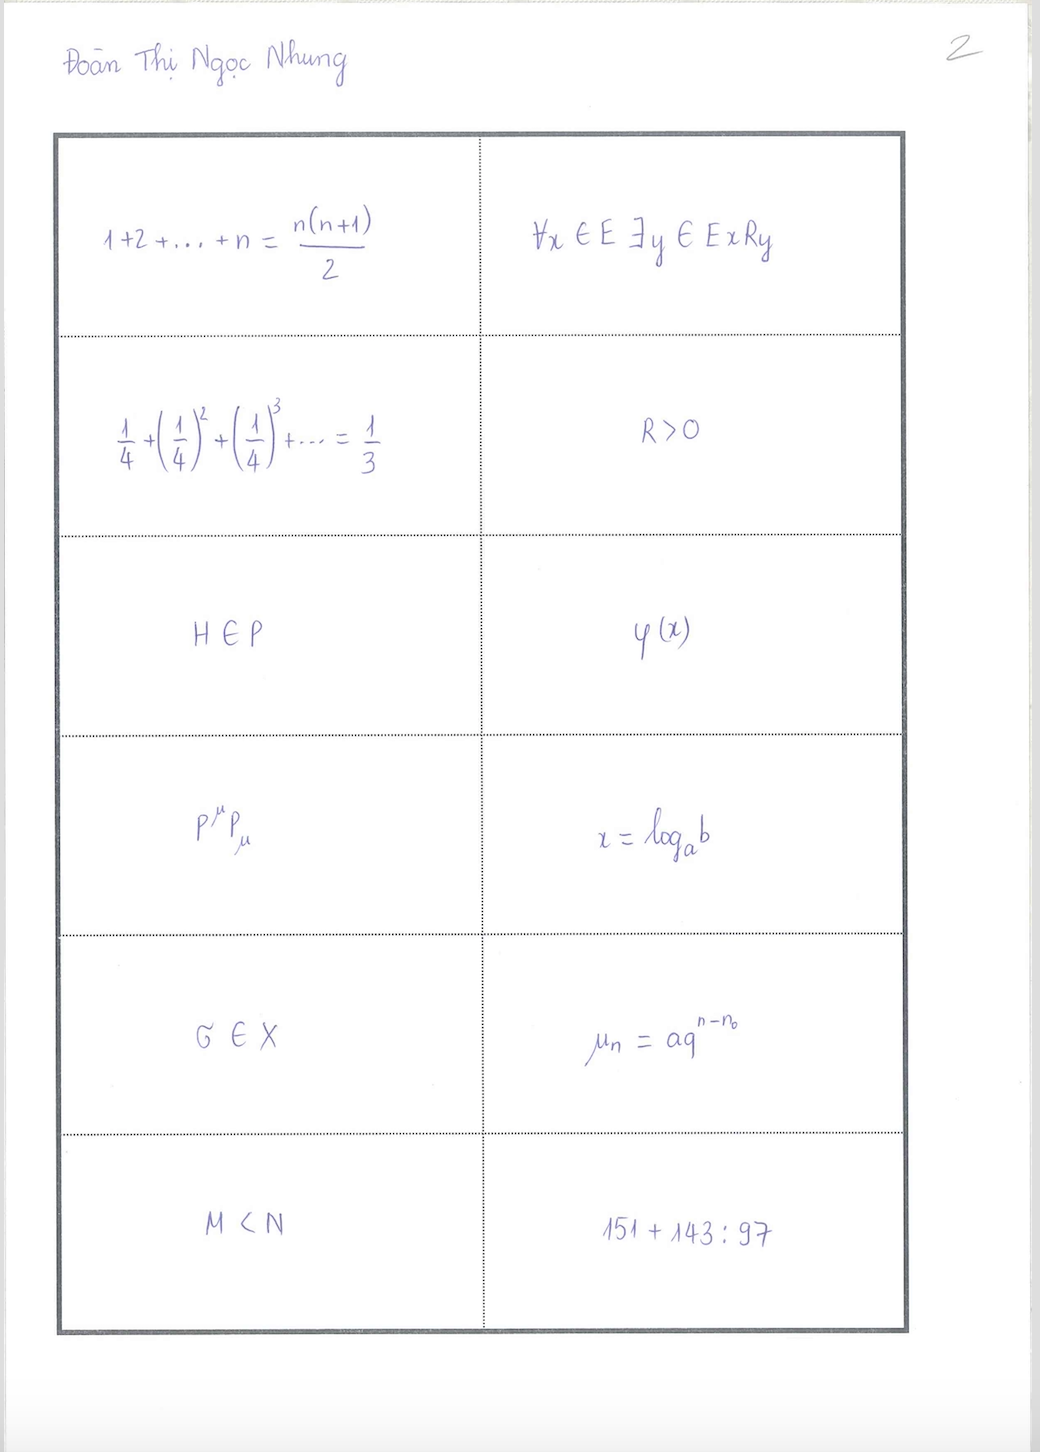
\includegraphics[width=0.8\linewidth]{Exp_sample_vd}
			\vspace{0.5cm}
			\captionof{figure}{Ví dụ một mẫu thu thập được từ người tham gia viết.}
		\end{center}
		\item Tập hợp lại các biểu mẫu sau khi cho người tham gia viết rồi mang đi scan. Sau đó xử lý qua một đoạn mã Matlab\cite{qak}\footnote{Đoạn mã này đã được chỉnh sửa để phù hợp với hình dạng mẫu lấy biểu thức của nhóm.} để từ một ảnh gồm nhiều biểu thức thu được ảnh chỉ chứa đúng một biểu thức như hình bên dưới. Ảnh này là ảnh xám, với kích thước $300\times300$.
		\begin{center}
			\centering
			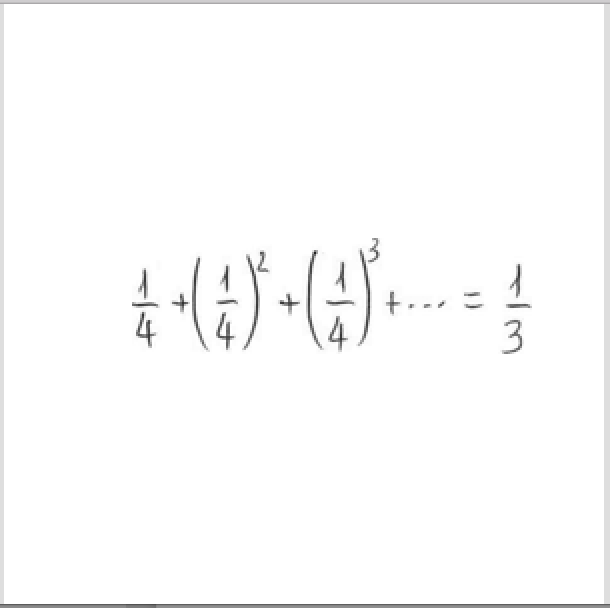
\includegraphics[width=0.5\linewidth]{EXP_2017_072_2A.png}
			\vspace{0.5cm}
			\captionof{figure}{Ví dụ một ảnh thu được sau khi xử lý biểu mẫu đã qua scan bằng đoạn mã Matlab.}
		\end{center}
		\item Thực hiện gán nhãn và xác định bounding box cho từng ký hiệu trong ảnh thu được từ bước trên bằng công cụ do nhóm tự thực hiện với giao diện như hình bên dưới. Công cụ này cho phép tải ảnh, xác định bounding boxes cho các đối tượng trong ảnh bằng cách kéo thả chuột từ góc trên bên trái đến góc dưới bên phải của từng đối tượng và nhập nhãn cho mỗi đối tượng đó. Quá trình này kết thúc sẽ thu được file với định dạng .txt lưu thông tin cần thiết về dữ liệu cho quá trình huấn luyện và kiểm tra. 
		\begin{center}
			\centering
			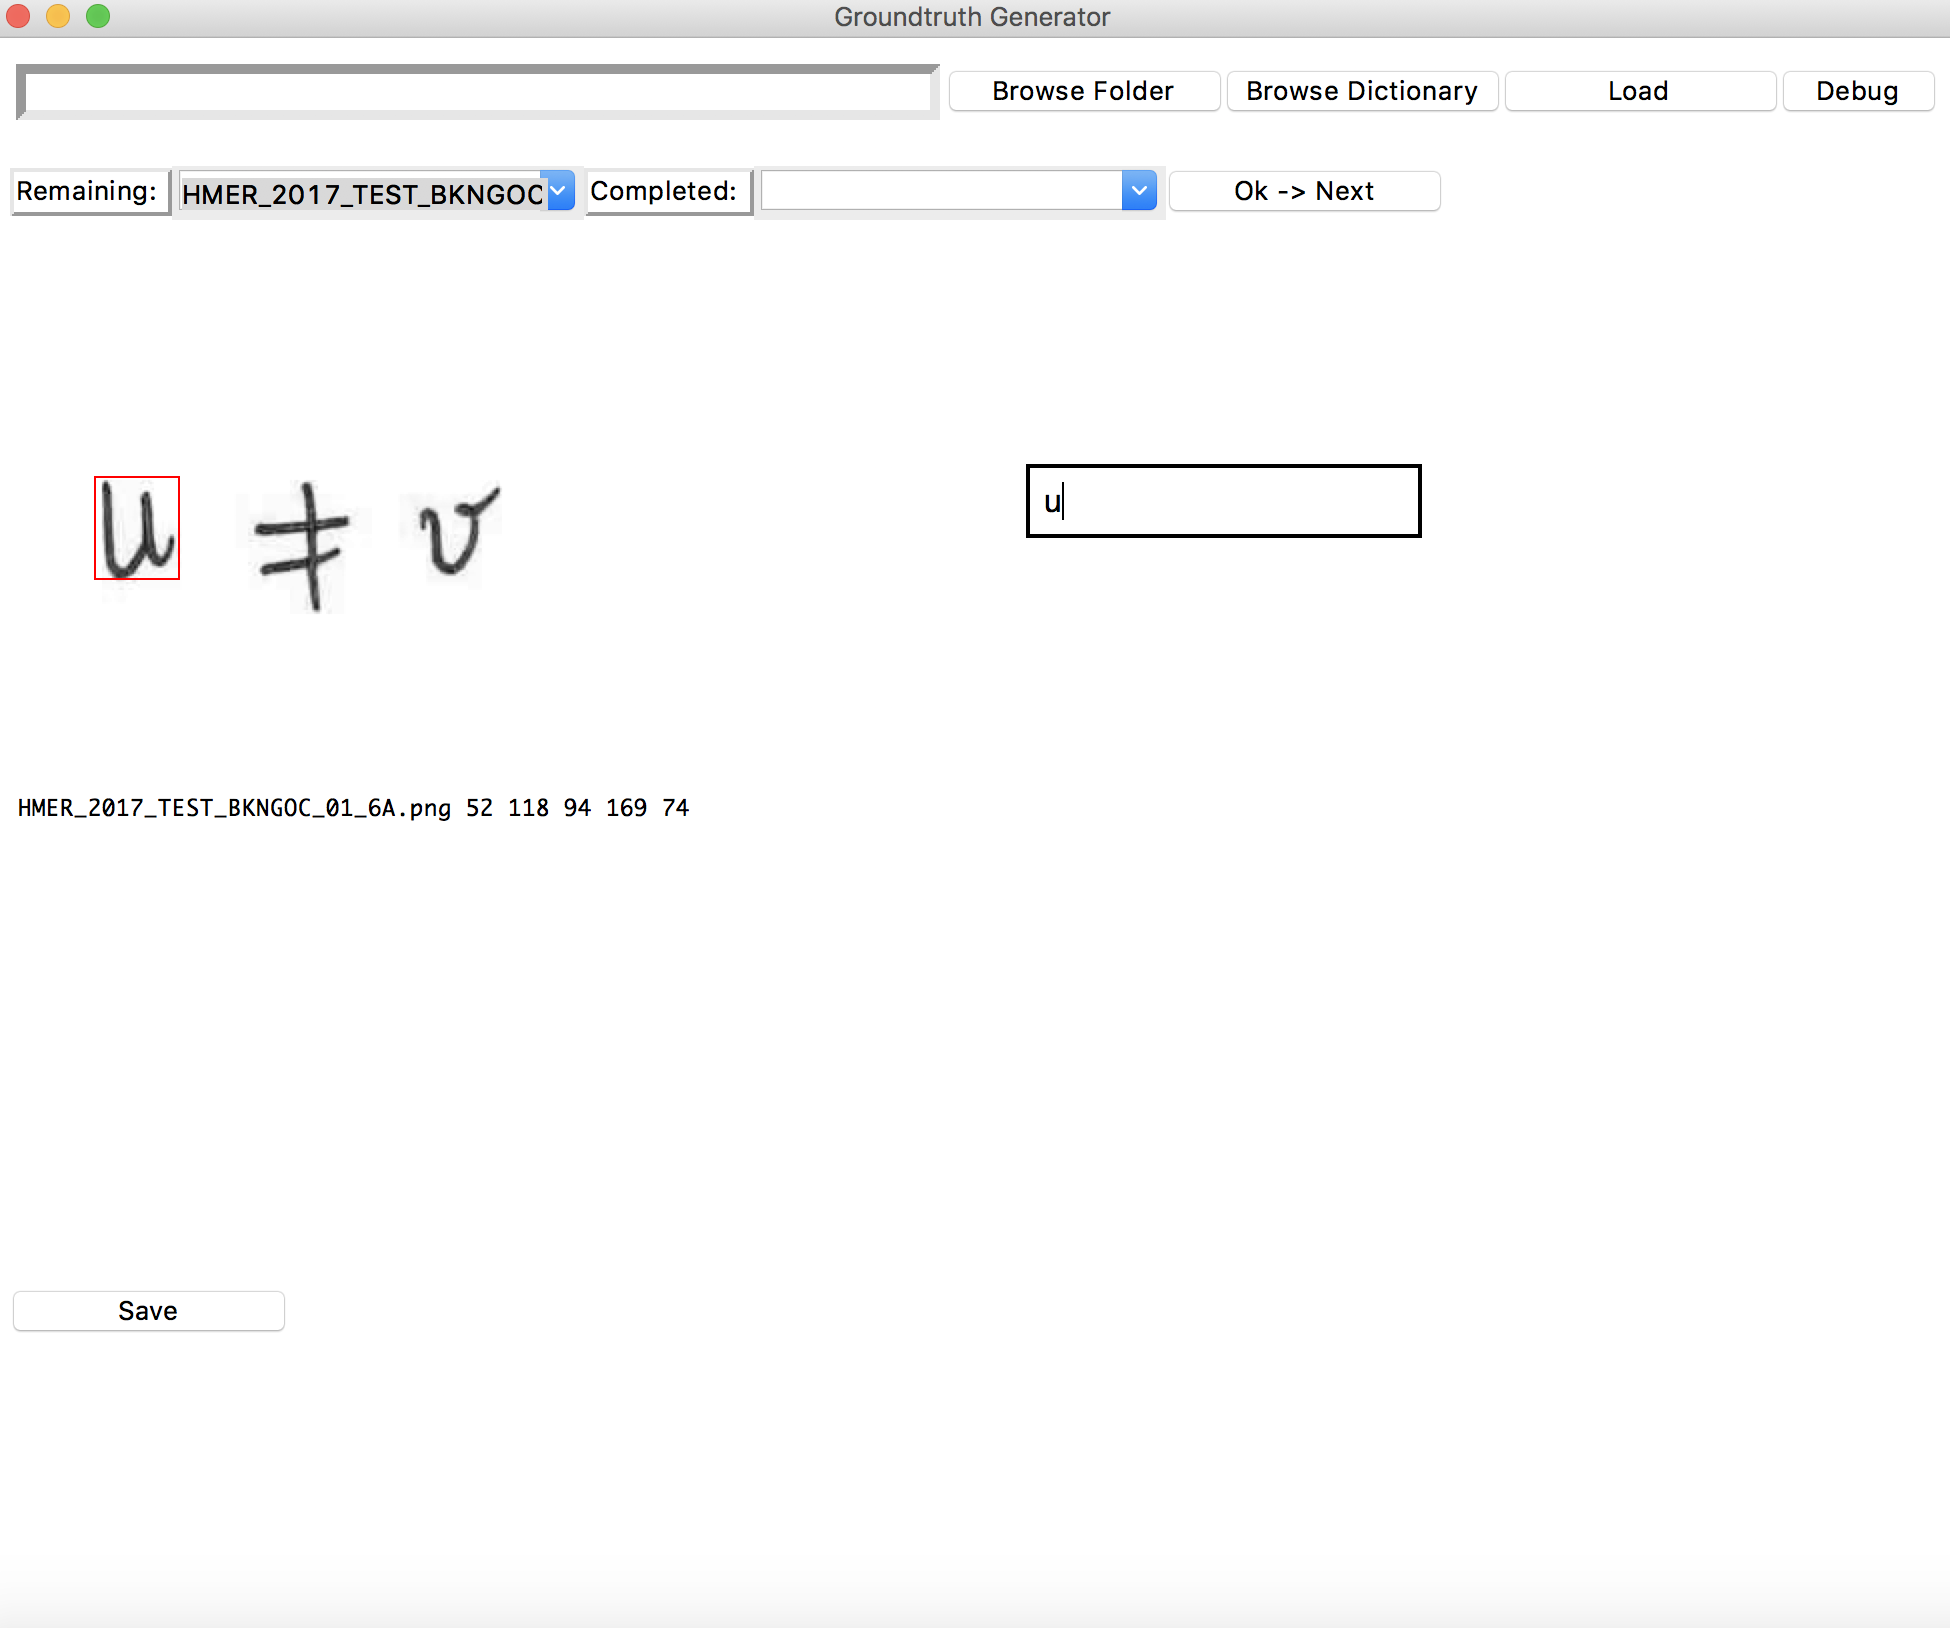
\includegraphics[width=0.65\linewidth]{tool}
			\vspace{0.5cm}
			\captionof{figure}{Giao diện công cụ hỗ trợ quá trình gán nhãn và xác định bounding boxes. }
		\end{center}
	\end{itemize}
	\subsubsubsection{Thông tin mô tả tập dữ liệu biểu thức}
	\begin{itemize}
		\item Số người tham gia: khoảng 88 
		\item Số lượng ảnh\footnote{Mỗi ảnh chỉ chứa một biểu thức.}:  2256 với 1746 ảnh dùng cho training, 138 ảnh dùng cho quá trình validation và 372 ảnh để test.
		Trong đó, 372 ảnh test được thu thập từ 2 nguồn:
		\begin{itemize}
		 	\item 192 ảnh được viết bởi người chưa từng tham gia viết cho quá trình thu thập ảnh huấn luyện.
		 	\item 102 ảnh còn lại được viết bởi 15 người đã tham gia quá trình thu thập ảnh huấn luyện.
		\end{itemize}
		\item Số loại biểu thức: khoảng 552
		\item Số  người gán nhãn: 3
	\end{itemize}
	\begin{center}
		\begin{tabular}{||c | c | c ||} 
			\hline
			 Thông tin thêm & Tập huấn luyện & Tập kiểm tra\\[0.5ex] 
			\hline\hline
			\makecell{Tổng số ký tự} & 13697 & 2237 \\
			\hline
			\makecell{Chiều dài trung bình\\ của biểu thức} &$\approx{8}$  &$\approx{6}$\\
			\hline
			\makecell{Kích thước trung bình\\ của ký tự}& $24\times29$&$31\times41$\\
			\hline
		\end{tabular}
		\captionof{table}{Thông tin mô tả hai tập dữ liệu dùng cho huấn luyện và kiểm tra.}
	\end{center}
	Hình minh hoạ cho sự phân phối số lượng ký tự trong từng nhãn đối với tập huấn luyện và tập kiểm tra.
	\begin{figure}
		
		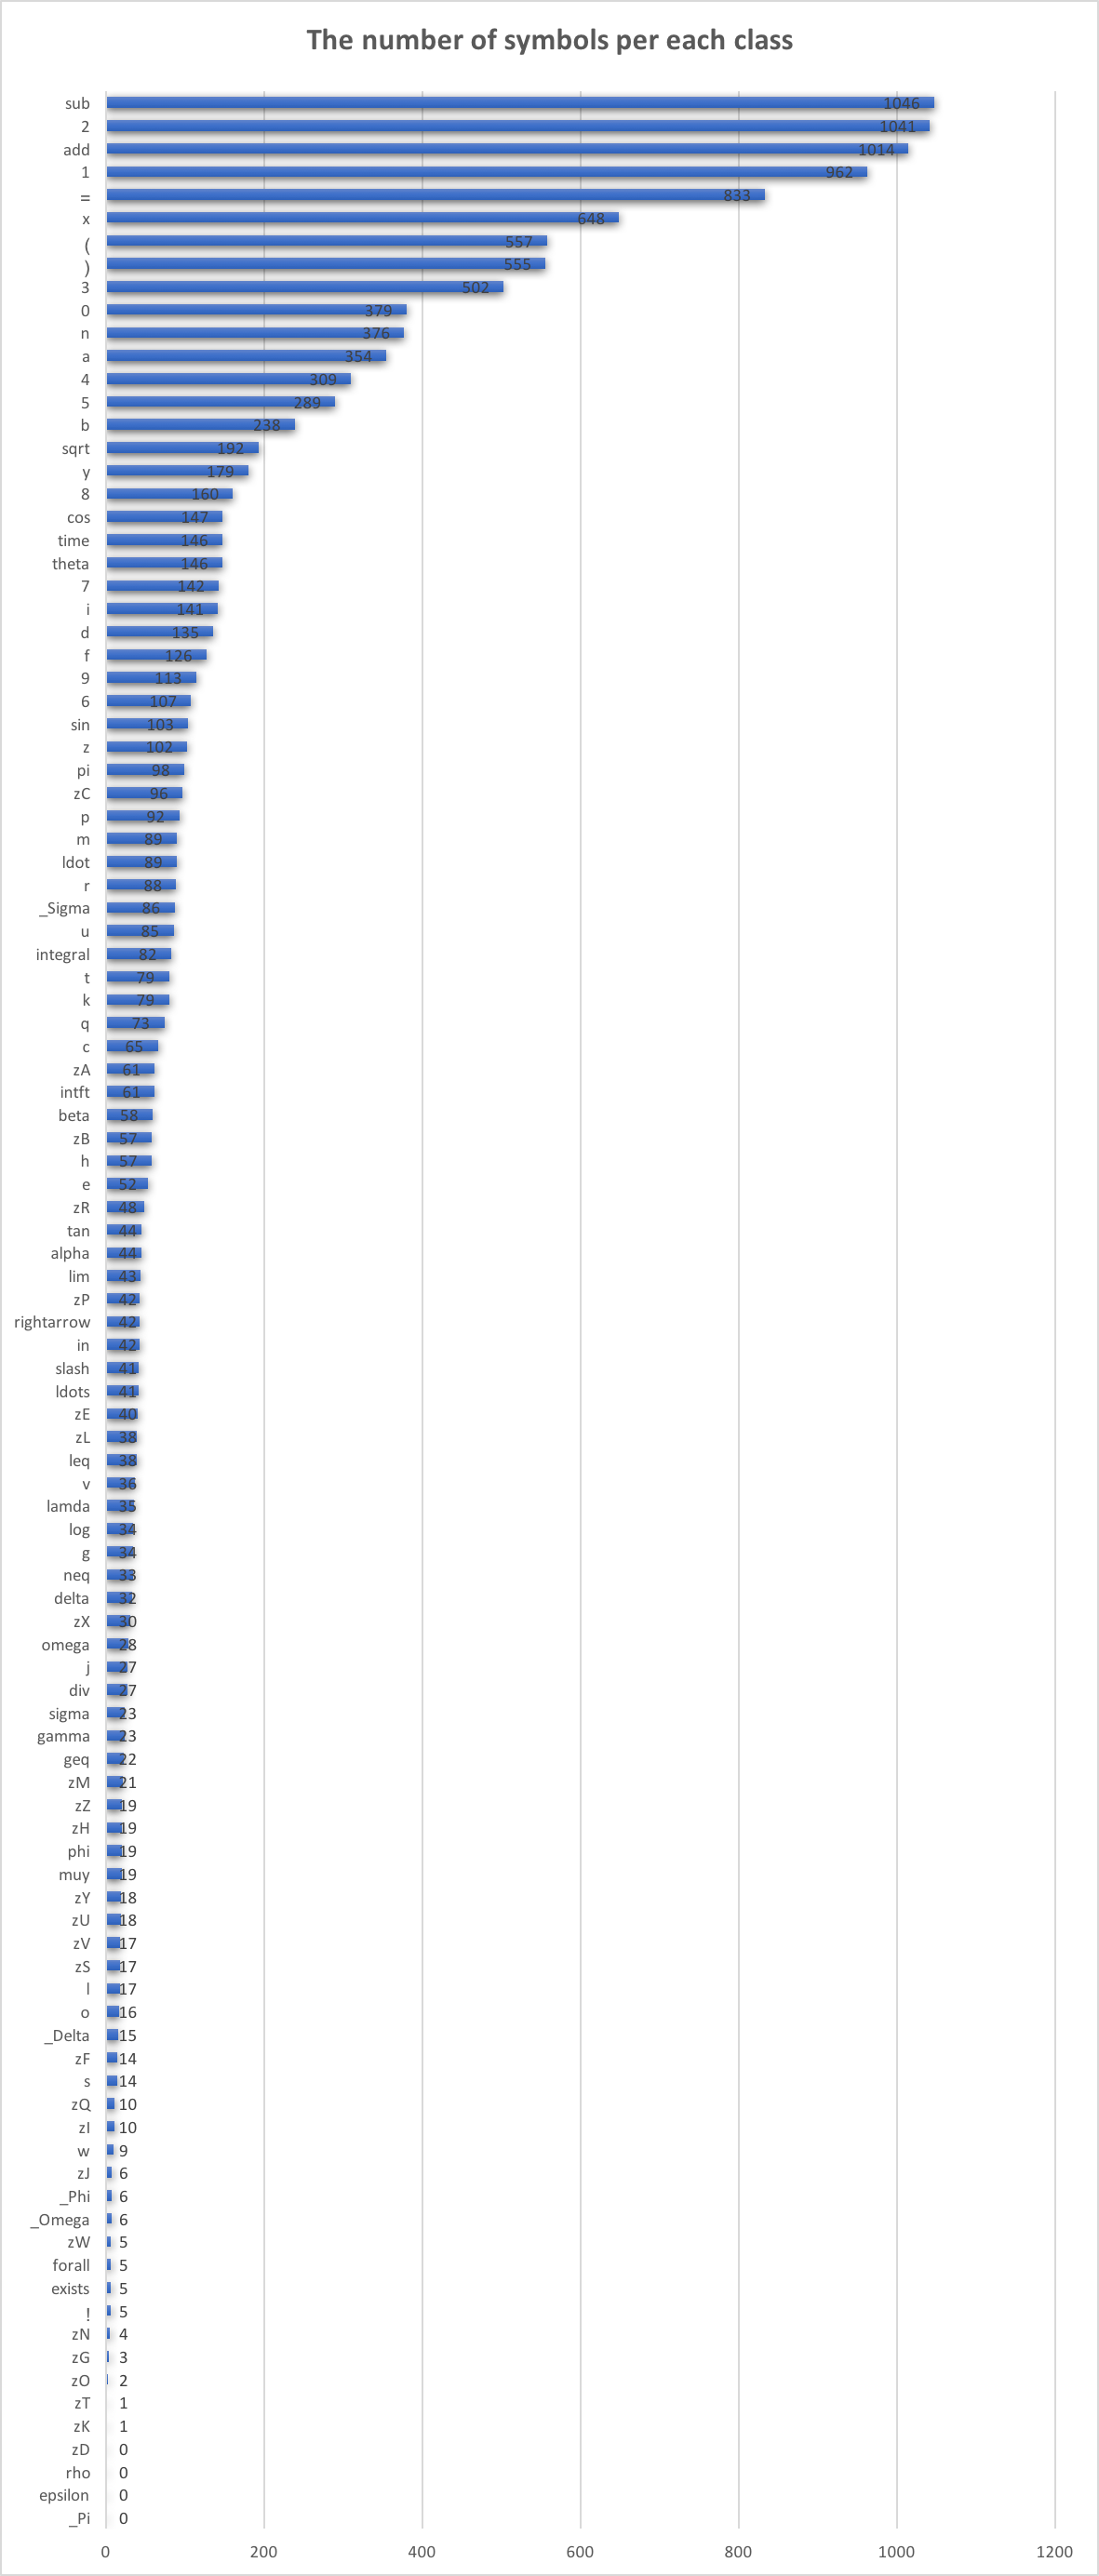
\includegraphics[width=0.475\linewidth]{train_statis.png}
		\hfill
		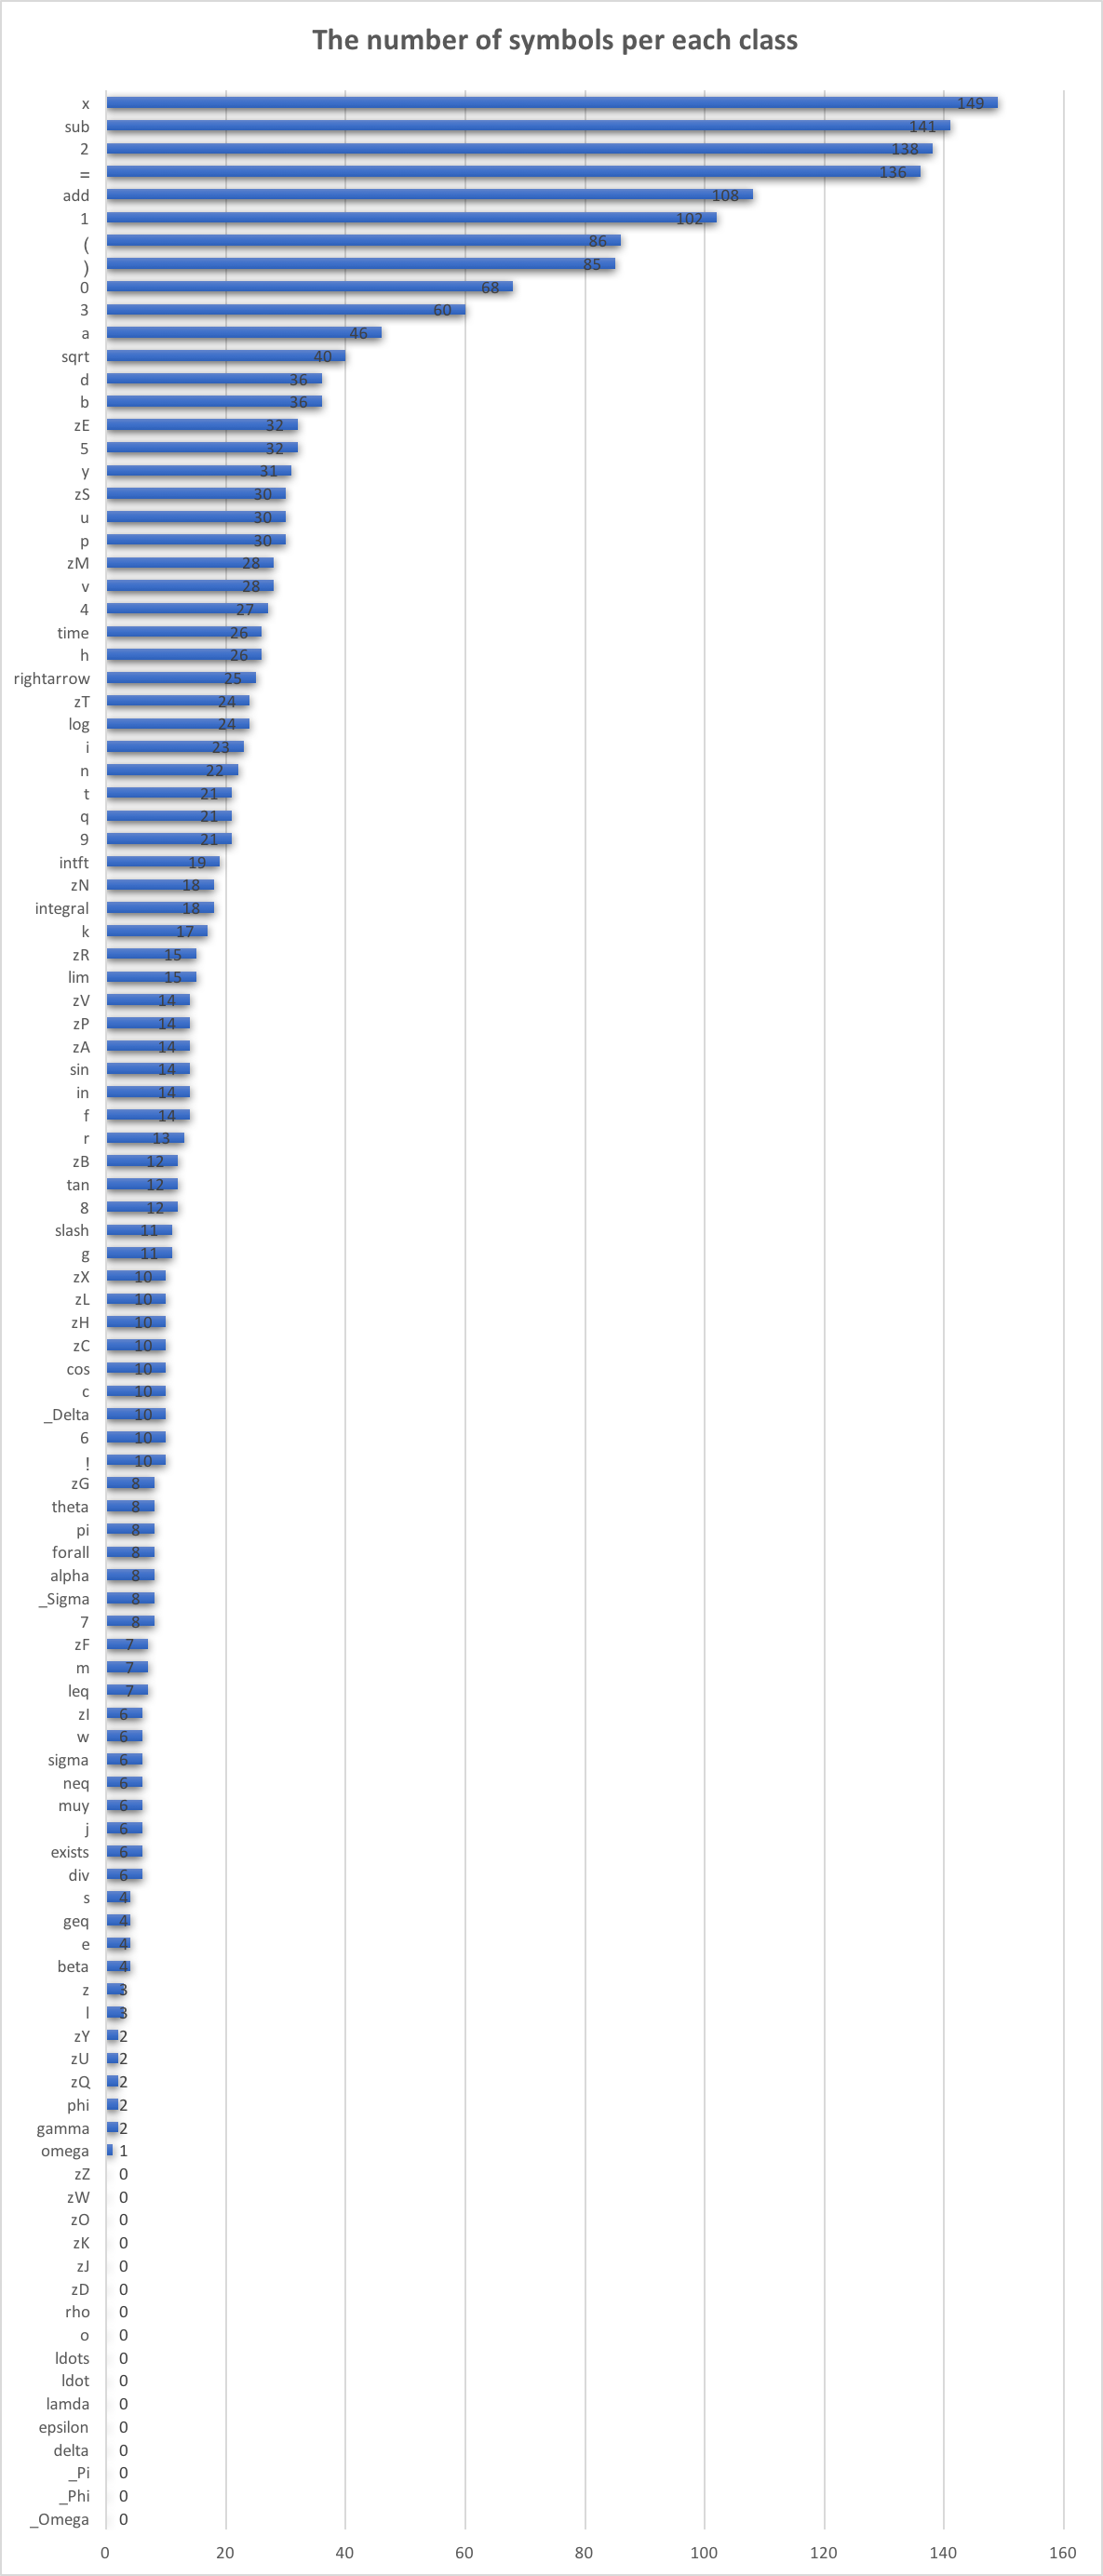
\includegraphics[width=0.475\linewidth]{test_statis.png}
		\vspace{0.5cm}
		\captionof{figure}{Sự phân phối ký tự theo từng nhãn đối với tập huấn luyện và tập kiểm tra.}
		\label{fig: distribution}
	\end{figure}
	
	\newpage
	\subsection{Xây dựng mô hình}
	\label{subsec: xaydungmohinh}
	Do bản chất mạng SSD300\cite{liu2016ssd} mô tả trong phần mô hình đề xuất gặp rất nhiều khó khăn trong việc nhận dạng ký tự nhỏ với một số lý do:
	\begin{itemize}
		\item Trong quá trình matching, các bounding box ground truth khi match với các default box phải có chỉ số Jaccard\cite{Jaccard} lớn hơn 0.5, nhưng kích thước tối thiểu của default box lại là $30 \times 30$ pixel, vì vậy nhiều ký tự nhỏ không thể match được (Trường hợp này xãy ra với hầu hết những ảnh có chữ nhỏ, ví dụ như ảnh dưới)
		\begin{center}
			\centering
			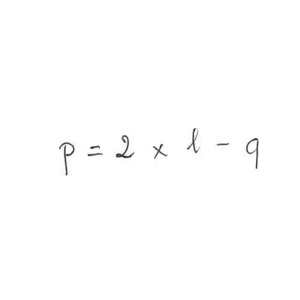
\includegraphics[resolution=300]{HMER_2017_TEST1_MINH_01_2A.png}
			\vspace{0.5cm}
			\captionof{figure}{Ảnh ví dụ chữ nhỏ (với kích thước thật)}
		\end{center}
		Khi không thể match được thì vùng ký tự đó được hiểu là phần nền, điều này gây bất lợi lớn cho quá trình huấn luyện do vùng ảnh không trống nhưng lúc là nền lúc lại được gắn nhãn.
		
		\item Nhiều ký tự có aspect ratio đặc biệt (Ví dụ như ký tự dấu $-$ trong phân số hoặc $\int$) cũng gặp nhiều khó khăn trong việc matching do không đạt được ngưỡng Jaccard\cite{Jaccard}.
	\end{itemize}
	Vì vậy, nhóm đã sửa một số thông số để tìm cách giải quyết vấn đề trên, trong nhiều bộ thông số thì có 3 phiên bản nổi bật sẽ được đặc tả bên dưới. Để thuận tiện, nhóm xin phép được đặt tên phiên bản SSD300 nguyên thủy\cite{liu2016ssd} với sự thiết lập đã được giới thiệu trong \ref{sec: mohinhdexuat} là phiên bản I. Phiên bản này được xây dựng dựa trên mã nguồn của tác giả tại \cite{github}. Ba phiên bản được dể xuất sau được đặt tên lần lượt là phiên bản II, III, IV.
	
	\subsubsection{Giảm kích thước các default box - Phiên bản II}
	
	Phiên bản này dựa trên phiên bản SSD300 nguyên thủy\cite{liu2016ssd}, chỉ chỉnh sửa kích thước các bounding box thông qua chỉnh hai thông số $s_{min} = 0.08$ và $s_{max} = 0.5$, từ đó danh sách kích thước các default box được thay đổi thành (9, 24, 54, 84, 114, 144, 174). So với phiên bản nguyên thủy, phiên bản này không thể match tốt các ký tự lớn (lớn hơn khoảng $200 \times 200$ pixel). Tuy vậy, đối với bài toán về phát hiện các ký tự trong một ảnh, thì kích thước các ký tự không thể quá lớn, nên những ký tự đặc biệt lớn như vậy có thể được xem xét ở độ ưu tiên thấp hơn.\\
	Việc thay đổi tham số ở phiên bản này không làm ảnh hưởng lớn đến cấu trúc mạng cũng như quá trình mã hóa, giải mã. Số lượng dự đoán không thay đổi.\\
	Mục đích chính của thay đổi này là để quá trình matching diễn ra tốt hơn khi kích thước của default box nhỏ nhất là $9 \times 9$, điều này giúp cho những ký tự rất nhỏ vẫn có thể được match, tránh hiện tượng bỏ sót ký tự như mạng SSD300 nguyên thủy\cite{liu2016ssd}.
	
	\subsubsection{Giảm kích thước các default box và tăng kích thước ảnh đầu vào - Phiên bản III}
	
	Để có được phiên bản này, nhóm cần phải có hai thay đổi so với mạng SSD300 nguyên thủy\cite{liu2016ssd}:
	\begin{itemize}
		\item Thay vì sử dụng ảnh $300 \times 300$ như nguyên thủy, ảnh sẽ được phóng to lên kích thước $500 \times 500$.
		\item Như ở phiên bản đề xuất trước, nhóm thay đổi $s_0 = 0.03$, $s_{min} = 0.08$ và $s_{max} = 0.5$ từ đó thu được danh sách kích thước (15.0, 40, 80, 120, 160., 200, 240, 280).
	\end{itemize}
	Những thay đổi trên có làm thay đổi đến cấu trúc mạng SSD\cite{liu2016ssd}, khi tăng kích thước ảnh đầu vào nghĩa là kích thước của các feature map thu thập được cũng tăng lên, từ đó kéo số lượng dự đoán trong một ảnh tăng lên như bảng dưới.\\
	
	\begin{center}
		\begin{tabular}{||c | c | c | c ||} 
			\hline
			\makecell{ Feature map \\ Sinh bởi } & \makecell{ Kích thước} & \makecell{Aspect Ratio } &  \makecell{ Số dự đoán } \\ [0.5ex] 
			\hline\hline
			Conv\_4 & $512 \times 63 \times 63$ & $ \{ 1, \frac{1}{2} , 2\} $ & 15876 \\ 
			\hline
			Conv\_7 & $1024 \times 32 \times 32$ & $ \{ 1, \frac{1}{2} , 2, \frac{1}{3}, 3\} $ & 6144 \\ 
			\hline
			Conv\_8 & $512 \times 16 \times 16$ &  $ \{ 1, \frac{1}{2} , 2, \frac{1}{3}, 3\} $ & 1536 \\ 
			\hline
			Conv\_9 & $256 \times 8 \times 8 $ &  $ \{ 1, \frac{1}{2} , 2, \frac{1}{3}, 3\} $ & 384  \\ 
			\hline
			Conv\_10 & $256 \times 4 \times 4$ & $ \{ 1, \frac{1}{2} , 2\} $ & 144 \\ 
			\hline
			Conv\_11 & $256 \times 2 \times 2$ & $ \{ 1, \frac{1}{2} , 2\} $ & 64 \\ 
			\hline
		\end{tabular}
		\captionof{table}{Thông tin của các feature map trích được từ mạng SSD đã giảm kích thước default box và tăng kích thước ảnh đầu vào}
	\end{center}
	Như vậy với mỗi ảnh, hệ thống sinh ra 24148 dự đoán, gấp gần 3 lần so với ảnh SSD300 nguyên thủy\cite{liu2016ssd}. Với những thay đổi này bounding box thậm chí còn có thể match với những default box nhỏ hơn, bên cạnh đó, mật độ các default box cũng dày đặc hơn nhiều so với mạng SSD nguyên thủy\cite{liu2016ssd}.
	
	\begin{center}
		\centering
		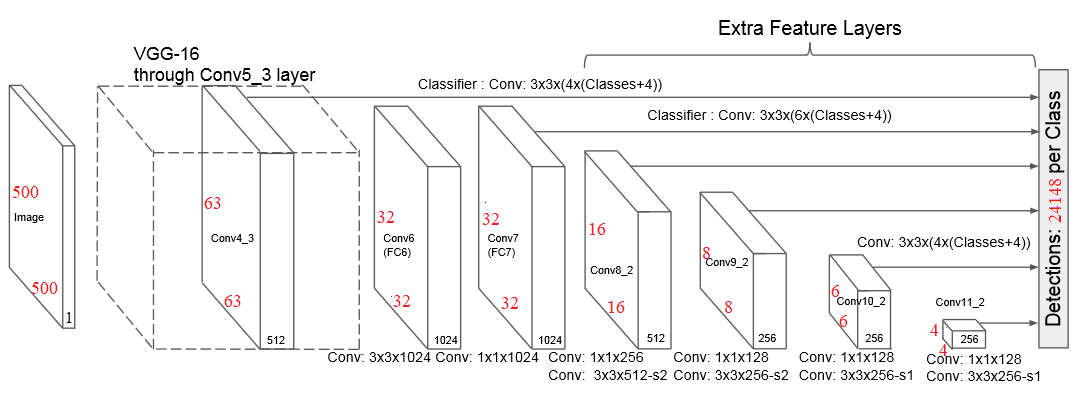
\includegraphics[width=0.875\linewidth]{SSD_Struture_4.png}
		\vspace{0.5cm}
		\captionof{figure}{Cấu trúc mạng của phiên bản III}
	\end{center}
	
	\subsubsection{Giảm kích thước các default box, tăng kích thước ảnh đầu vào và thêm lớp tích chập - Phiên bản IV}
	
	Phiên bản này thừa kế các thay đổi ở hai phiên bản trước, tuy nhiên ở phần thân mạng SSD\cite{liu2016ssd}, nhóm đã gắn thêm 2 lớp tích chập ở cuối với các tham số: \\
	
	\begin{center}
		\begin{tabular}{||c | c | c | c | c | c ||} 
			\hline
			Khối & \makecell{ Số kênh \\ đầu vào } & \makecell{ Số kênh \\ đầu ra} & Kích thước nhân &  \makecell{ Chèn thêm \\ (Padding) } &  \makecell{ Bước \\ (Stride) } \\ [0.5ex] 
			\hline\hline
			Conv\_12\_1 & 256 & 128 & 1 & 0 & 1 \\ 
			\hline
			Conv\_12\_2 & 128 & 256 & 3 & 0 & 1 \\ 
			\hline
		\end{tabular}
		\captionof{table}{Cấu hình các lớp tích chập thêm vào mạng SSD300\cite{liu2016ssd} để được mạng SSD chỉnh sửa}
	\end{center}
	Hai lớp tích chập này cũng có hàm truyền là hàm relu và đi chung với lớp dropout\cite{srivastava2014dropout} với hệ số dropout là 0.2. \\
	
	Thay đổi này cũng làm thay đổi cấu trúc mạng:
	
	\begin{center}
		\begin{tabular}{||c | c | c | c ||} 
			\hline
			\makecell{ Feature map \\ Sinh bởi } & \makecell{ Kích thước} & \makecell{Aspect Ratio } &  \makecell{ Số dự đoán } \\ [0.5ex] 
			\hline\hline
			Conv\_4 & $512 \times 63 \times 63$ & $ \{ 1, \frac{1}{2} , 2\} $ & 15876 \\ 
			\hline
			Conv\_7 & $1024 \times 32 \times 32$ & $ \{ 1, \frac{1}{2} , 2, \frac{1}{3}, 3\} $ & 6144 \\ 
			\hline
			Conv\_8 & $512 \times 16 \times 16$ &  $ \{ 1, \frac{1}{2} , 2, \frac{1}{3}, 3\} $ & 1536 \\ 
			\hline
			Conv\_9 & $256 \times 8 \times 8 $ &  $ \{ 1, \frac{1}{2} , 2, \frac{1}{3}, 3\} $ & 384  \\ 
			\hline
			Conv\_10 & $256 \times 4 \times 4$ & $ \{ 1, \frac{1}{2} , 2\} $ & 64 \\ 
			\hline
			Conv\_11 & $256 \times 2 \times 2$ & $ \{ 1, \frac{1}{2} , 2\} $ & 16 \\ 
			\hline
			Conv\_12 & $256 \times 2 \times 1$ & $ \{ 1, \frac{1}{2} , 2\} $ & 4 \\ 
			\hline
		\end{tabular}
		\captionof{table}{Thông tin của các feature map trích được từ mạng SSD\cite{liu2016ssd} đã giảm kích thước default box, tăng kích thước ảnh đầu vào và tăng số lớp tích chập}
	\end{center}
	Lớp Conv\_12 được thêm vào cuối mạng với mục đích tăng độ dài danh sách feature map đưa vào lớp Multibox, điều này giúp trong quá trình matching, các ký tự lớn hơn có thể được match.
	
	\begin{center}
		\centering
		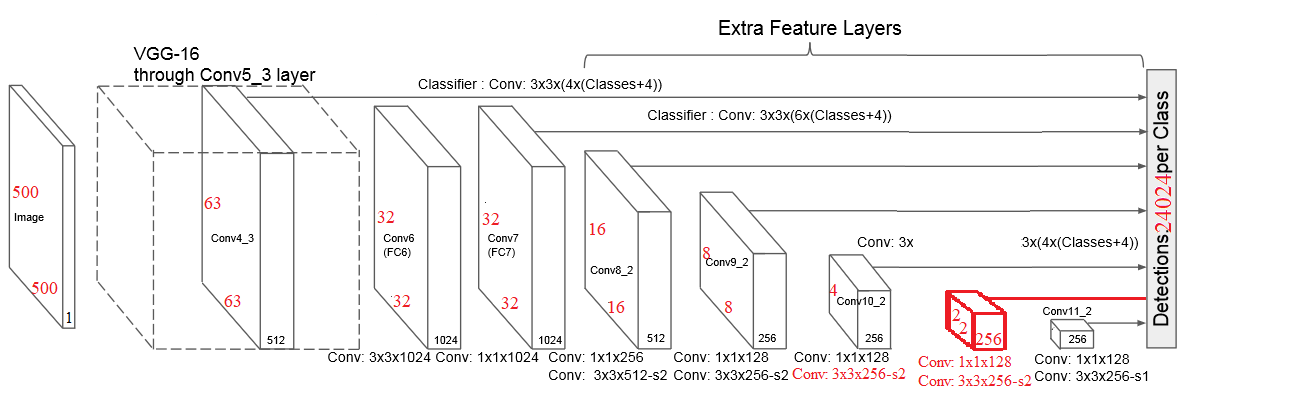
\includegraphics[width=0.875\linewidth]{SSD_Struture_5.png}
		\vspace{0.5cm}
		\captionof{figure}{Cấu trúc mạng của phiên bản III}
	\end{center}
	
	\subsection{Xây dựng bản thử nghiệm}
	
	Khi đã thu được mô hình hoàn thiện của SSD, nhóm xây dựng một bản thử nghiệm bằng python. Giao diện khá đơn giản, người dùng chỉ việc chọn thư mục chứa ảnh, sau đó chọn ảnh cần nhận diện. Chương trình sẽ xử lý và đưa ra 3 ảnh gồm ảnh gốc ban đầu, ảnh thể hiện các bounding box mà mạng dự đoán và ảnh biểu thức toán học được tạo ra từ đoạn mã Latex.
	
	\begin{center}
		
		\centering
		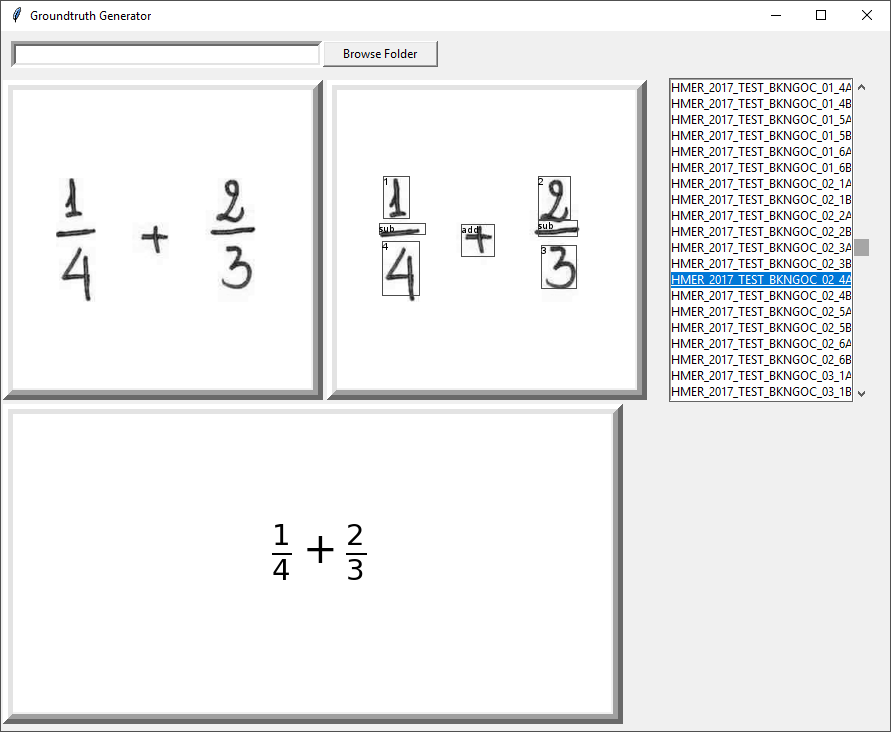
\includegraphics[width=0.8\linewidth]{demoImg.png}
		\vspace{0.5cm}
		\captionof{figure}{Giao diện bản thử nghiệm}
	\end{center}
	\subsection{Kết quả}
	
	
	\subsubsection{So sánh định tính giữa bốn phiên bản}
	\subsubsubsection{Quá trình matching}
	Nhóm đã giảm kích thước các default box, đồng thời phóng to ảnh đầu vào, một phần mục đích là để quá trình matching có thể thực hiện tốt hơn đối với các ký tự nhỏ. Công việc này thật sự đã cải thiện được quá trình matching khi kích thước tối thiểu của bounding box ground truth được cải thiện một cách đáng kể:
	
	\begin{center}
		\begin{tabular}{||c | c | c | c | c||} 
			\hline
			Mô hình & \makecell{  I } & \makecell{ II} & III &  \makecell{ IV}  \\ [0.5ex] 
			\hline
			bounding box vuông & $22 \times 22$ & $12 \times 12$ & $7 \times 7$ & $7 \times 7$ \\
			\hline
			bounding box có tỉ lệ 1 : 2 & $16 \times 32$ & $16 \times 32$ & $5 \times 10$ & $5 \times 10$ \\
			\hline
		\end{tabular}
		\captionof{table}{Kích thước bounding box ground truth nhỏ nhất mà mạng có thể match với default box được của bốn mô hình đề xuất. (Đơn vị tính: Điểm ảnh - Pixel) }
	\end{center}
	
	\subsubsubsection{Quá trình nhận diện}
	
	Kết quả của phiên bản II không tốt, về mặt lý thuyết thì khi giảm kích thước các bounding box, khả năng nhận diện các ký tự nhỏ sẽ tốt hơn, tuy nhiên khi áp dụng cho phiên bản II, mạng đã gặp một số vấn đề: 
	
	\begin{itemize}
		\item Giảm kích thước bounding box sẽ khiến cho các ký tự lớn "bị hổng", do các bounding box quá lớn khi tính chỉ số Jaccard\cite{Jaccard} với các default box quá nhỏ sẽ không đủ ngưỡng, vì vậy mạng không thể match được các ký tự lớn, từ đó mạng cũng không thể nhận diện các ký tự lớn.
		\item Mạng có thể nhận diện được các ký tự nhỏ hơn, tuy nhiên các ký tự này cũng không đủ nhỏ để bao phủ phần lớn các ký tự nhỏ có trong tập dữ liệu.
	\end{itemize}
	Vì vậy, qua thực nghiệm, phiên bản II đưa ra dự đoán về ký tự nhỏ tốt hơn phiên bản I một ít, nhưng kết quả vẫn còn rất tệ. Tuy vậy đối với những ký tự lớn, phiên bản II tỏ ra yếu hơn so với phiên bản I.\\
	Ngược lại với phiên bản II, kết quả của phiên bản III và IV khá tốt, hệ thống đã có thể nhận diện nhiều ký tự rất nhỏ và tương đối chuẩn xác, phiên bản IV hầu như không thua kém phiên bản I trong việc nhận diện ký tự lớn, một số ký tự phiên bản I nhận diện được nhưng phiên bản IV không thể và ngược lại. Để hoàn thiện phiên bản III, IV trong việc nhận diện ký tự lớn, nhóm có đề xuất một hướng đi trong tương lai để cải thiện khả năng nhận diện ký tự lớn này.\\
	
	\begin{center}
		\centering
		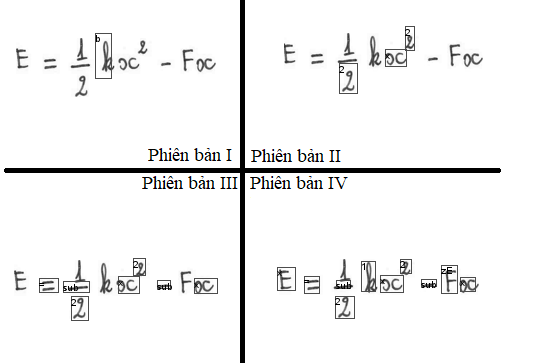
\includegraphics[width=0.8\linewidth]{compare_1.png}
		\vspace{0.5cm}
		
		\captionof{figure}{Kết quả dự đoán của 4 phiên bản. Khả năng nhận diện ký tự nhỏ tăng dần qua 4 phiên bản. (1)}
	\end{center}
	
	\begin{center}
		\centering
		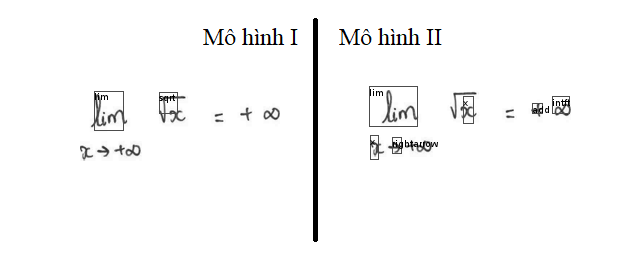
\includegraphics[width=0.775\linewidth]{compare_2.png}
		\vspace{0.5cm}
		
		\captionof{figure}{Kết quả dự đoán của 4 phiên bản. Khả năng nhận diện ký tự nhỏ tăng dần qua 4 phiên bản. (2)}
	\end{center}
	
	\begin{center}
		\centering
		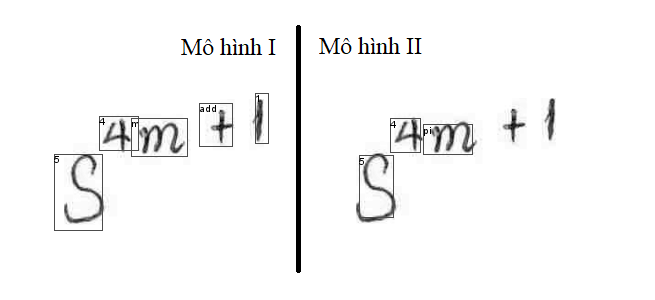
\includegraphics[width=0.775\linewidth]{compare_4.png}
		\vspace{0.5cm}
		
		\captionof{figure}{Kết quả dự đoán của 4 phiên bản. Phiên bản III và IV tỏ ra vượt trội hai phiên bản trước.}
	\end{center}
	
	\begin{center}
		\centering
		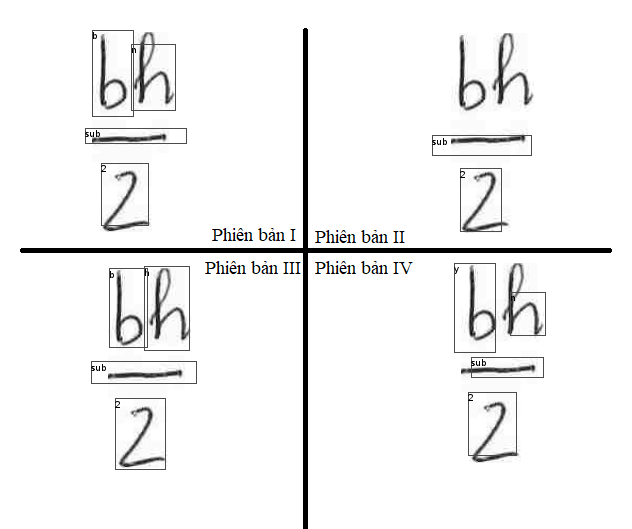
\includegraphics[width=0.775\linewidth]{compare_3.png}
		\vspace{0.5cm}
		
		\captionof{figure}{Kết quả dự đoán của 4 phiên bản. Khả năng nhận diện ký tự lớn giảm mạnh ở phiên bản II.}
	\end{center}
	
	\begin{center}
		\centering
		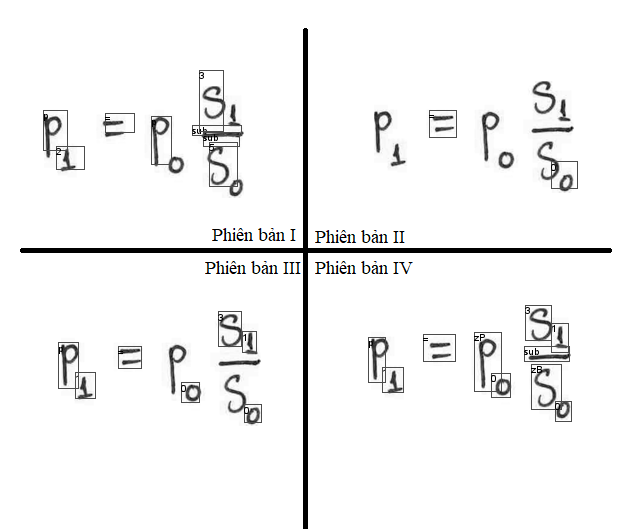
\includegraphics[width=0.775\linewidth]{compare_5.png}
		\vspace{0.5cm}
		
		\captionof{figure}{Kết quả dự đoán của 4 phiên bản. Khả năng nhận diện ký tự lớn ở phiên bản IV không thua kém phiên bản I.}
	\end{center}
	Đặc biệt, có nhiều biểu thức có ký tự rất nhỏ nhưng phiên bản IV đã làm việc rất tốt:
	
	\begin{center}
		\centering
		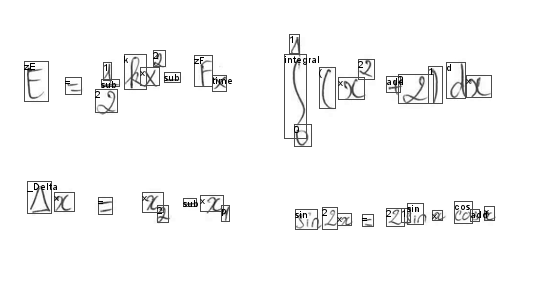
\includegraphics{compare_7.png}
		\vspace{0.5cm}
		\captionof{figure}{Ảnh kết quả của phiên bản IV(với kích thước thật)}
	\end{center}
	
	
	
	\subsubsection{So sánh định đlượng}
	Trong quá trình thực hiện, nhóm đã xây dựng 4 phiên bản huấn luyện dựa trên những thay đổi của 3 yếu tố sau:
	\begin{itemize}
		\item Kích thước ảnh đầu vào của mạng SSD.
		\item Kích thước default boxes.
		\item Số lượng default boxes.
	\end{itemize}
	Thông tin cụ thể đã được trình bày ở phần \ref{subsec: xaydungmohinh} của chương này, bên dưới là bảng tóm tắt.
	\begin{center}
		\begin{tabular}{||c | c | c | c | c||} 
			\hline
			Phiên bản & \makecell{  I } & \makecell{ II} & III &  \makecell{ IV}  \\ [0.5ex] 
			\hline\hline
			Kích thước ảnh đầu vào& 300x300 & 300x300 & 500x500 & 500x500 \\ 
			\hline
			Kích thước default boxes& \makecell{min\_ratio: 20\\max\_ration: 90\\min\_scale: 0.1} &  \makecell{min\_ratio: 8\\max\_ratio: 50\\min\_scale: 0.03} & \makecell{min\_ratio: 8\\max\_ratio: 50\\min\_scale: 0.03}  & \makecell{min\_ratio: 8\\max\_ratio: 50\\min\_scale: 0.03}  \\ 
			\hline
			Số lượng default boxes & 8732 & 8732 & 24148 & 24024\\
			\hline
		\end{tabular}
		\captionof{table}{Sự khác nhau giữa 4 phiên bản thử nghiệm.}
	\end{center}
	Điều kiện đánh giá:
	\begin{itemize}
		\item Cùng một tập ảnh kiểm tra với 372 ảnh. Phân phối số lượng ký tự trên từng nhãn của tập ảnh kiểm tra được thể hiện trong Hình \ref{fig: distribution}.
		\item Độ đo sử dụng: mAP\\
		Cách tính:\\ Tính precision cho từng nhãn theo công thức\cite{mAP}:
		\begin{align}
		precision = \frac{TP}{TP+FP},
		\end{align}
		\hspace{2cm}với $TP$ được viết tắt từ $True Positive$\cite{mAP} và $FP$ từ $False Positive$\cite{mAP}.\\
		Tính trọng số của từng nhãn trong tập dữ liệu kiểm tra theo công thức:
		\begin{align}
		class\_weight_i = \frac{N_i}{\sum_{u=0}^{106}N_u},
		\end{align}
		\hspace{2cm}với $N_i$ là số lượng ký tự thuộc nhãn $i$.\\
		mAP là trung bình có trọng số giữa $precision$ và $class\_weight$.
		\item Điều kiện máy chạy đánh giá:
		\begin{itemize}
			\item Hệ điều hành: Ubuntu 14.04 LTS
			\item CPU: Intel Core i5- 2500M 3.30GHz 
			\item RAM: 8GB
		\end{itemize}
	\end{itemize}
	Kết quả đánh giá của 4 phiên bản:
	\vspace{0.5cm}
	\begin{center}
		\begin{tabular}{||c | c | c | c | c||} 
			\hline
			Phiên bản & I&II&III&IV\\[0.5ex] 
			\hline\hline
			mAP&0.58036471&0.505290245&0.63949538&0.65268642\\
			\hline
			\makecell{Số lượng ký tự\\ nhận dạng được}&1581&1054&1837&1920\\
			\hline
			\makecell{Số file ảnh\\ không xử lý được}&4/372&8/372&0/372&0/372\\
			\hline
		\end{tabular}
		\captionof{table}{Kết quả mAP của 4 phiên bản thử nghiệm.}
	\end{center}
	\vspace{1.5cm}
	\begin{center}
		\centering
		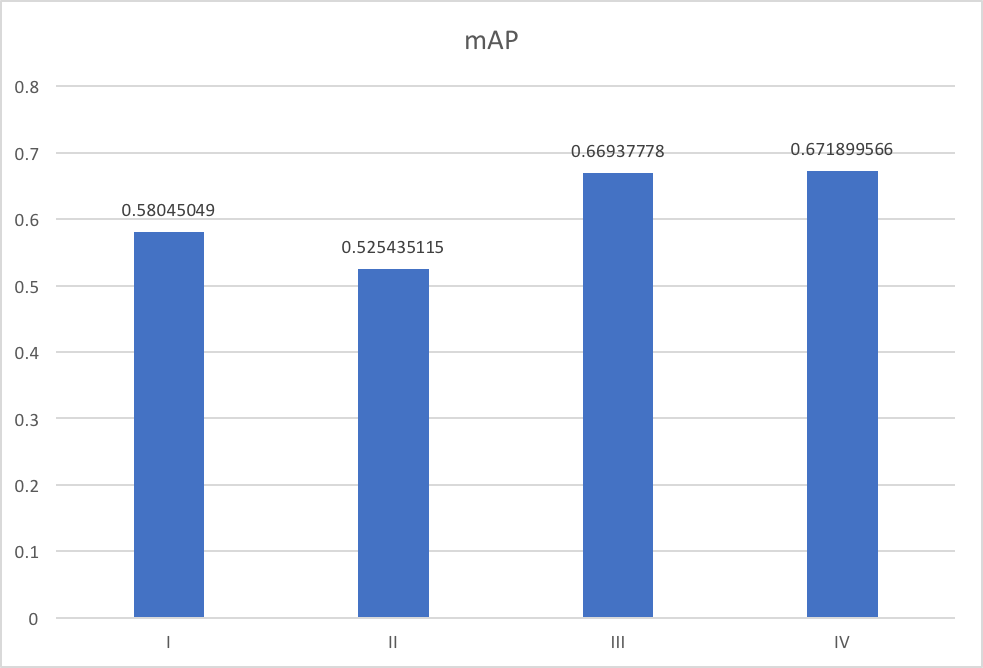
\includegraphics[width=0.775\linewidth]{mAP.png}
		\vspace{0.5cm}
		\captionof{figure}{Trực quan kết quả mAP cho 4 phiên bản thử nghiệm.}
	\end{center}
	Như vậy, từ mô hình ban đầu- mô hình I- với những thiết lập được giữ y nguyên như \cite{liu2016ssd}, nhóm đã thay đổi để tạo ra được mô hình IV- mô hình tốt nhất của nhóm. Từ đó nâng chỉ số mAP từ khoảng $58\%$ lên khoảng $65\%$. Nhìn vào đánh giá giữa 4 mô hình, rõ ràng thấy được việc thay đổi kích thước ảnh đầu vào và kích thước default box có tác động mạnh đến việc cải thiện độ chính xác của phương pháp. 
	\vspace{1cm}
	\begin{center}
		\centering
		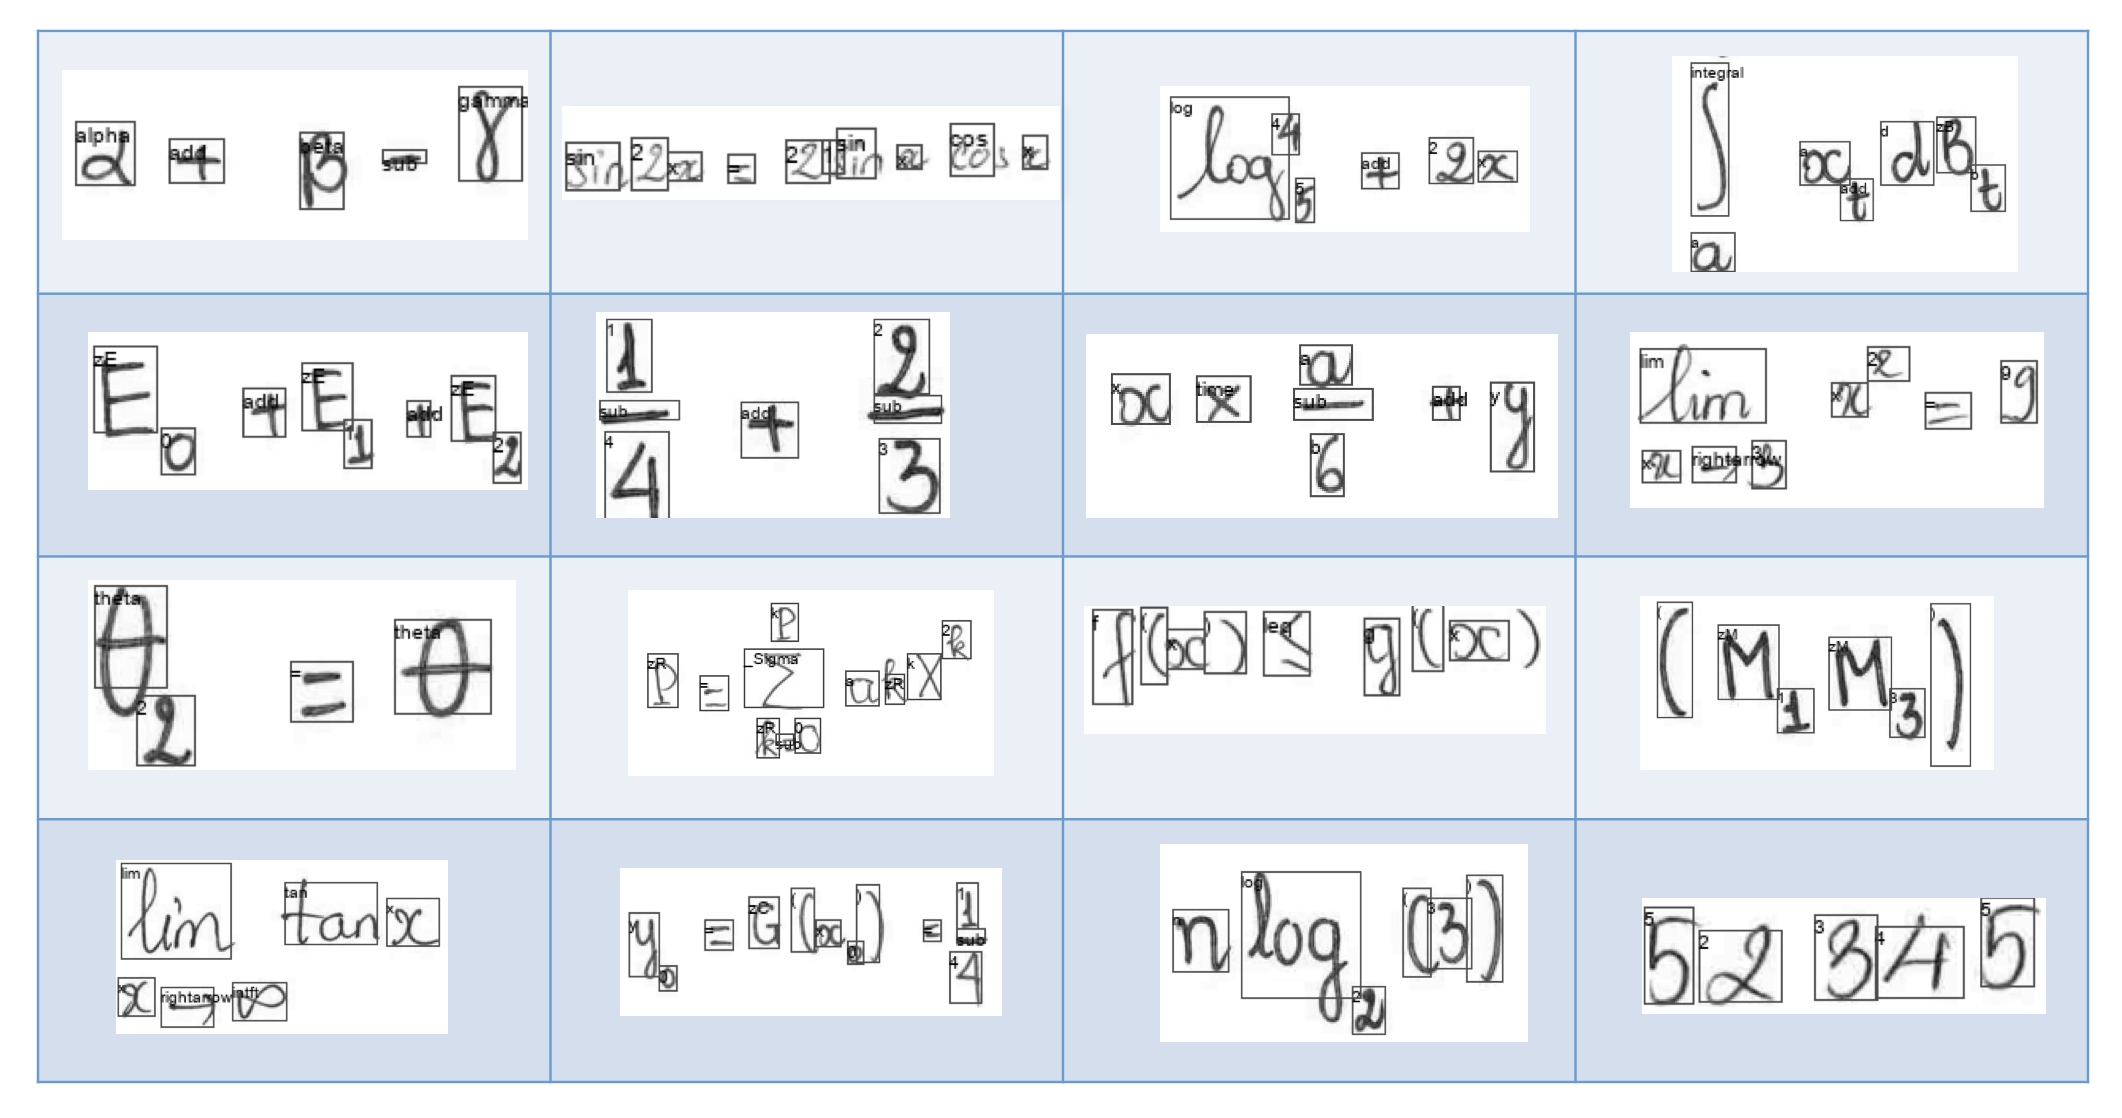
\includegraphics[width=0.99\linewidth]{result}
		\vspace{0.5cm}
		\captionof{figure}{Một số ảnh kết quả sau quá trình nhận dạng sử dụng phiên bản IV.}
	\end{center}
	%%%%%%%%%%%%%%%%%%%%%%%%%%%%%%%%%%%%%
	%%%%%%%%%%%%%%%%%%%%%%%%%%%%%%%%%%%%%
	\newpage	
	\section{Tổng kết}
	
	\subsection{Kết luận}
	Hệ thống nhận dạng biệu thức toán học viết tay mà nhóm đang xây dựng là bước đầu cho một ứng dụng tiện ích sau này đối với các bạn học sinh, sinh viên cũng như với những giáo viên- những người thường xuyên tiếp xúc với các con số, công thức và mong muốn rằng có một sản phẩm nào đó hỗ trợ giải các bài toán không chỉ bằng cách đưa ra đáp số mà còn là hướng dẫn giải từng bước, vẽ đồ thị hàm số hay thậm chí cho phép tương tác lên hình ảnh đồ thị đó, gợi ý họ những đoạn lệnh Latex hay có thể là một ngôn ngữ tương tự từ ảnh của những biểu thức để tiết kiệm thời gian soạn thảo những công thức dài và phức tạp. Ngoài ra, với việc có thể trực quan những đồ thị hàm số hay hướng dẫn giải một số loại bài toán sẽ giúp cho việc dạy và học trở nên sinh động và thuận lợi hơn. Như vậy, rất rất nhiều những ứng dụng có thể phát triển từ hệ thống nhận dạng mà nhóm đang thực hiện. \\
	Với hệ thống này, nhóm đã sử dụng phương pháp phát hiện và nhận dạng của mạng SSD thay vì những phương pháp phân tách phổ biến như phân tích hình chiếu, phân tích thành phần liên thông để khắc phục những lỗi sai có thể xảy ra khi gặp những ký tự dính nhau, bọc lấy nhau kết hợp với bộ phân tích cấu trúc DRACULAE, hệ thống sẽ giải quyết được nhiều loại công thức phức tạp hơn như những công thức có chứa chỉ số trên, chỉ số dưới,... 
	Ngoài ra, trong quá trình thực hiện đề tài, nhóm đã phát triển 2 tập dữ liệu viết tay bao gồm 1 tập các ký tự và 1 tập những biểu thức từ đơn giản đến phức tạp. Với tập ký tự, dữ liệu đã lên tới con số 52353 file ảnh còn đối với tập biểu thức, hiện tại nhóm đã có khoảng 2400 ảnh. Đây là điều kiện quan trọng để nhóm có thể thực hiện những bước huấn luyện, đánh giá mô hình và cũng là cơ sở cho những đề tài liên quan đến chữ viết tay. 
	\subsection{Đánh giá ưu, nhược điểm}
	
	\subsubsection{Ưu điểm}
	
	\begin{itemize}
		\item Hệ thống có thể nhận diện được ký tự ở nhiều kích thước khác nhau.
		\item Nhận diện được nhiều biểu thức mà nếu chỉ dùng kỹ thuật phân vùng thì khó có thể làm được (ví dụ như biểu thức có ký tự dính nhau).
		\item Nhận diện được nhiều loại ký tự.
	\end{itemize}
	
	\subsubsection{Nhược điểm}
	
	\begin{itemize}
		\item Khi có nhiều ký tự trong ảnh thì hệ thống nhận diện gặp nhiều khó khăn.
		\item Tốc độ xử lý một ảnh còn chậm.
		\item Bộ phân tích cú pháp còn đơn giản.
		\item Các ký tự hoàn toàn trùng lên nhau dễ bị bỏ sót (dấu căn).
	\end{itemize}
	\subsection{Hướng phát triển trong tương lai}
	Đến thời điểm kết thúc luận văn, hệ thống mà nhóm xây dựng vẫn còn tồn tại những khuyết điểm và cả những trường hợp mà nhóm chưa có thời gian để kiểm tra. Trong đó nổi lên 2 vấn đề mà nhóm đã tiến hành giải quyết thử và thu được những kết quả khả quan ở bước đầu là việc thu nhỏ nội dung ảnh để có thể khắc phục lỗi sai mà hệ thống mắc phải khi gặp những ký tự quá lớn và tăng cường thêm dữ liệu để giải quyết trực tiếp vô trường hợp chỉ số dưới của 2 ảnh cụ thể trong tập test không nhận diện được. Ngoài ra vẫn còn nhiều trường hợp khác nữa mà theo nhóm đó là hướng phát triển trong tương lai của đề tài. 
	
	\subsubsection{Mở rộng tập dữ liệu biểu thức}
	Trong quá trình đánh giá hệ thống trên tập kiểm tra với mô hình IV, nhóm nhận thấy đối với 2 ảnh bên dưới hệ thống không nhận dạng được chỉ số dưới- cụ thể là số 1 ở vị trí dấu gạch đỏ. 
	\begin{center}
		\centering
		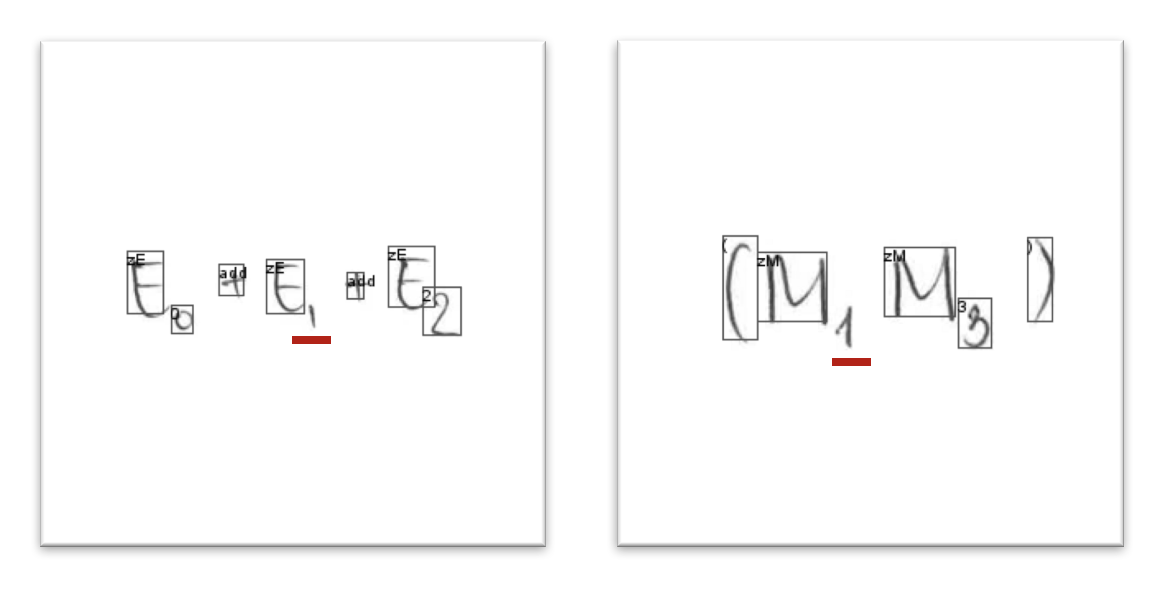
\includegraphics[width=0.6\linewidth]{M1E1}
		\vspace{0.5cm}
		\captionof{figure}{Trường hợp không nhận được chỉ số dưới.}
		\label{fig: m1}
	\end{center}
	Trên nhận định lý do của vấn đề này là do trong tập huấn luyện số lượng mẫu với chỉ số dưới còn ít và thiếu những mẫu mà chỉ số dưới dính vào hệ số của nó, nhóm đã bổ sung thêm 96 ảnh với nội dung cố định là $E_1$ và $M_1$ vào tập huấn luyện và 24 ảnh để kiểm tra với hy vọng sau khi huấn luyện lại với lượng ảnh bổ sung thì tình trạng trong Hình \ref{fig: m1} sẽ được giải quyết.\\
	Sử dụng kiến trúc mạng theo mô hình IV, sau quá trình huấn luyện với tập dữ liệu đã được thêm mới, nhóm thu được kết quả là cả 24 ảnh kiểm tra đều được nhận dạng đúng.
	\vspace{1cm}
	\begin{center}
		\centering
		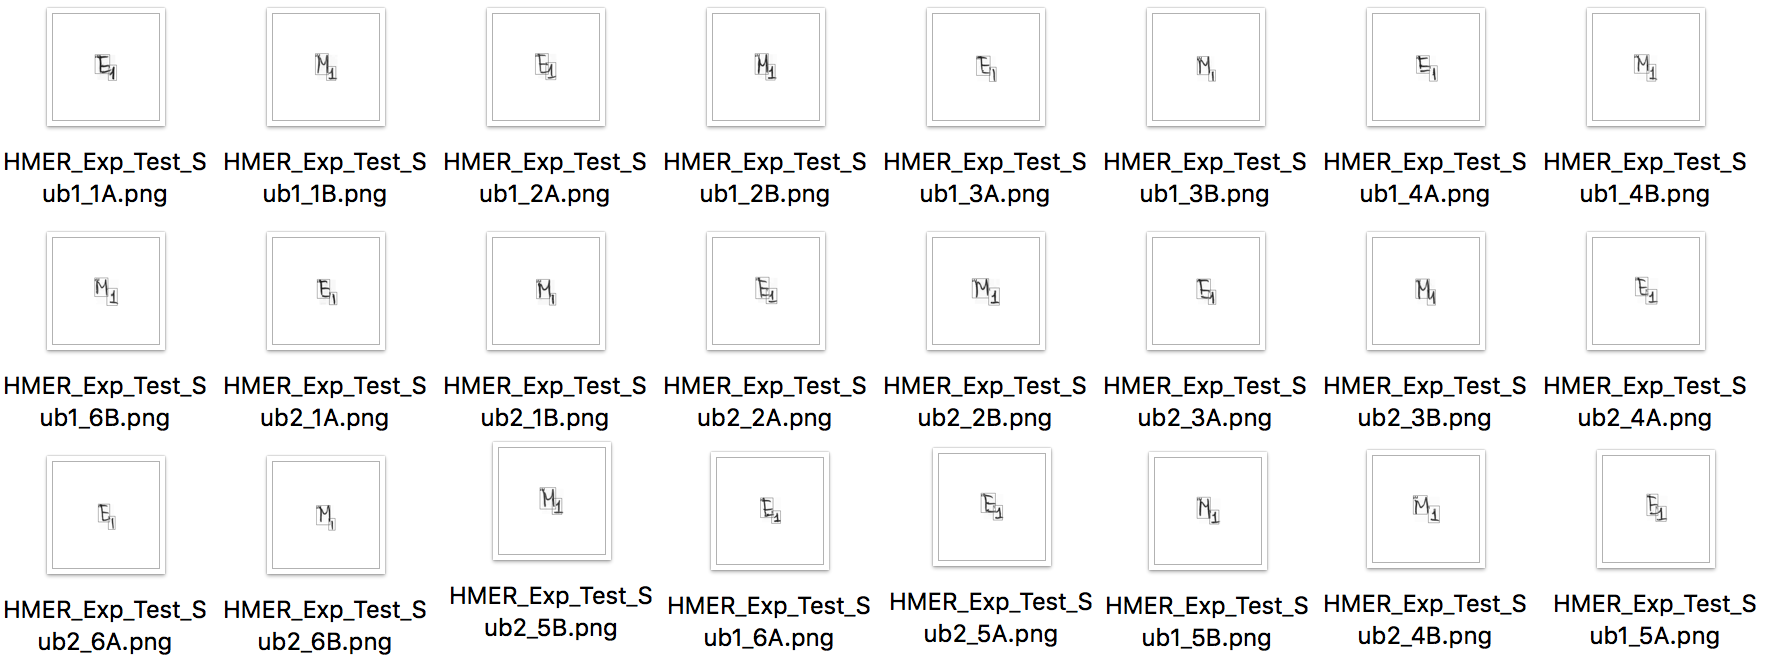
\includegraphics[width=0.7\linewidth]{subfolder}
		\vspace{0.5cm}
		\captionof{figure}{ Kết quả nhận dạng chỉ số dưới trên bộ ảnh test mới.}
	\end{center}
	Và kết quả trên 2 ảnh gặp lỗi ở Hình \ref{fig: m1}:
	\begin{center}
		\centering
		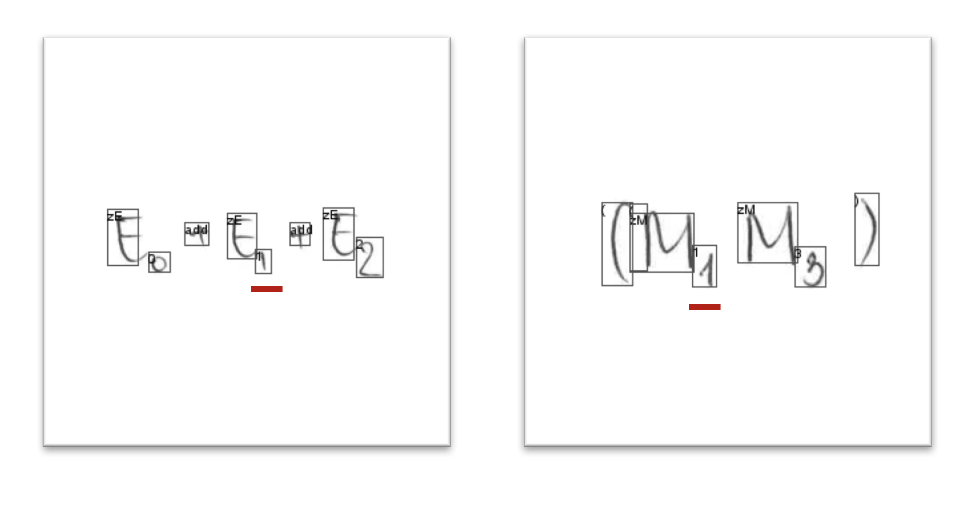
\includegraphics[width=0.7\linewidth]{M1E1_res}
		\vspace{0.5cm}
		\captionof{figure}{ Kết quả nhận dạng sau khi được huấn luyện với dữ liệu bổ sung.}
	\end{center}
	Có thể nhận thấy được rằng, ký tự tại vị trí dấu gạch đỏ ở cả 2 hình đều được phát hiện và nhận đúng. Do đó hướng giải quyết phát triển tập dữ liệu là điều cần thiết và khả năng sẽ khắc phục những một số lỗi sai khác. 
	\subsubsection{Khắc phục lỗi nhận dạng sai ở ký tự lớn}
	
	Như nhóm đã đề cập ở phần trước, phiên bản IV hoạt động chưa tốt với những ký tự quá lớn, nắm được điều này, nhóm đã thử thu nhỏ ảnh và tiến hành chèn thêm (padding) vào ảnh đã thu nhỏ đó để nội dung ảnh thì nhỏ lại nhưng kích thước ảnh không đổi, vẫn $500 \times 500$.
	
	\begin{center}
		\centering
		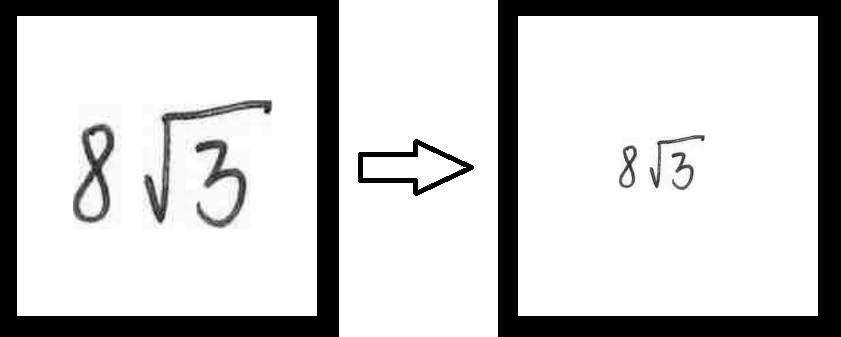
\includegraphics[width=0.775\linewidth]{ensmall.png}
		\vspace{0.5cm}
		
		\captionof{figure}{Ví dụ thu nhỏ ảnh.}
	\end{center}
	
	Sau khi thí nghiệm với một số ảnh, nhóm đã nhận thấy kết quả nhận được là khá tốt.
	
	\begin{center}
		\centering
		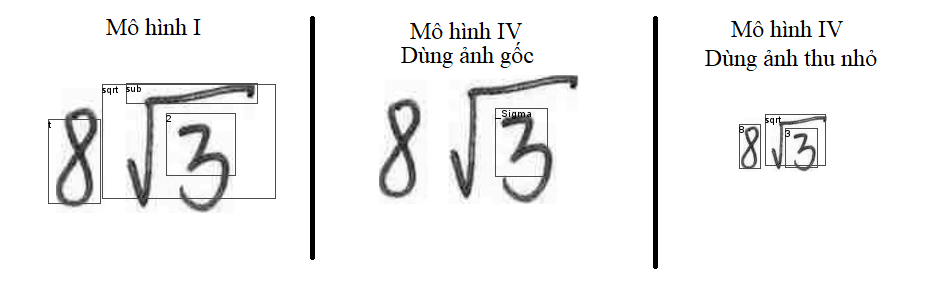
\includegraphics[width=0.875\linewidth]{compare_future.png}
		\vspace{0.5cm}
		
		\captionof{figure}{Kết quả thu được sau khi thu nhỏ nội dung ảnh.}
	\end{center}
	Vì vậy, một trong những điều cần được thực hiện ngay trong tương lai là tối ưu hoá bộ tiền xử lý để xử lý linh hoạt cho những ảnh có nội dung lớn và nhỏ khác nhau. Từ đó tạo ra bộ ảnh đầu vào phù hợp cho hệ thống.
	%Vì vậy, nhóm tin rằng có thể thêm vào hệ thống một bộ phận tiền xử lý có nhiệm vụ tự động thu nhỏ nội dung ảnh nếu cần và nếu phù hợp.
	
	\subsubsection{Các hướng phát triển khác}
	Như đã đề cập ở đầu mục này, vẫn còn nhiều trường hợp mà nhóm không có đủ thời gian để kiểm tra trong giai đoạn luận văn. Đây cũng là những hướng đi mà trong tương lai nhóm cần phải thực hiện. Cụ thể, nhóm chưa kiểm tra được liệu hệ thống của mình có thể hoạt động tốt trong các tình huống sau:
	\begin{itemize}
		\item Ảnh chứa đựng các ký tự nghiêng.
		\item Ảnh có nhiễu.
		\item Ảnh với nền khác màu trắng.
		\item Ảnh chụp thay vì scan.
		
	\end{itemize}
	\vspace{1cm}
	Ngoài ra, cũng còn những điều cần hoàn thiện:
	\begin{itemize}
		\item Thêm phần hậu xử lý ở các giai đoạn nhận diện ký tự và sinh cây Lexed - BST.
		\item Cải thiện khả năng nhận diện các ký tự có aspect ratio đặc biệt.
		\item Tối ưu hoá bộ phân tích cú pháp. 
	\end{itemize}
	
	\newpage
	\section*{Lời kết}
	Trải qua giai đoạn luận văn và cả thực tập tốt nghiệp, những thành viên nhóm đã học được nhiều điều. Về kiến thức, luận văn này là cơ hội cho các thành viên nhóm tìm hiểu và hiện thực những mô hình mạng Deep learning. Bước đầu biết được những vấn đề khó khăn khi huấn luyện một mạng và cách khắc phục chúng. Hiểu và xây dựng được một ứng dụng trên lĩnh vực nhận dạng đó chính là đề tài của nhóm, mặc dù về mặt ứng dụng nó còn ở mức đơn sơ. Về cách làm việc nhóm, trên thực tế các thành viên nhóm liên tục gặp phải những bất đồng, tranh chấp trên quan điểm làm việc cũng như xử lý vần đề. Có những lúc gay gắt mà các thành viên cảm thấy không thể tiếp tục được với nhau. Tuy nhiên tất cả những điều khó khăn này xảy ra đều dựa trên nền tảng vì một luận văn thành công, vì một đề tài mà cả hai thành viên nhóm đều tự hào nên đã vượt qua được. Tất cả những điều đó là trải nghiệm, là kinh nghiệm để các thành viên nhóm hoàn thiện mình hơn cho giai đoạn công việc sắp tới. Cho đến thời điểm này, mặc dù vẫn còn đó những thiếu sót nhưng cả 2 thành viên nhóm tự hào vì những điều mình đã làm được. \\
	Chân thành cảm ơn. 
	\newpage
	\section*{Phụ lục}
	\subsection*{Những lỗi sai mà hệ thống gặp phải}
		\begin{center}
		\centering
		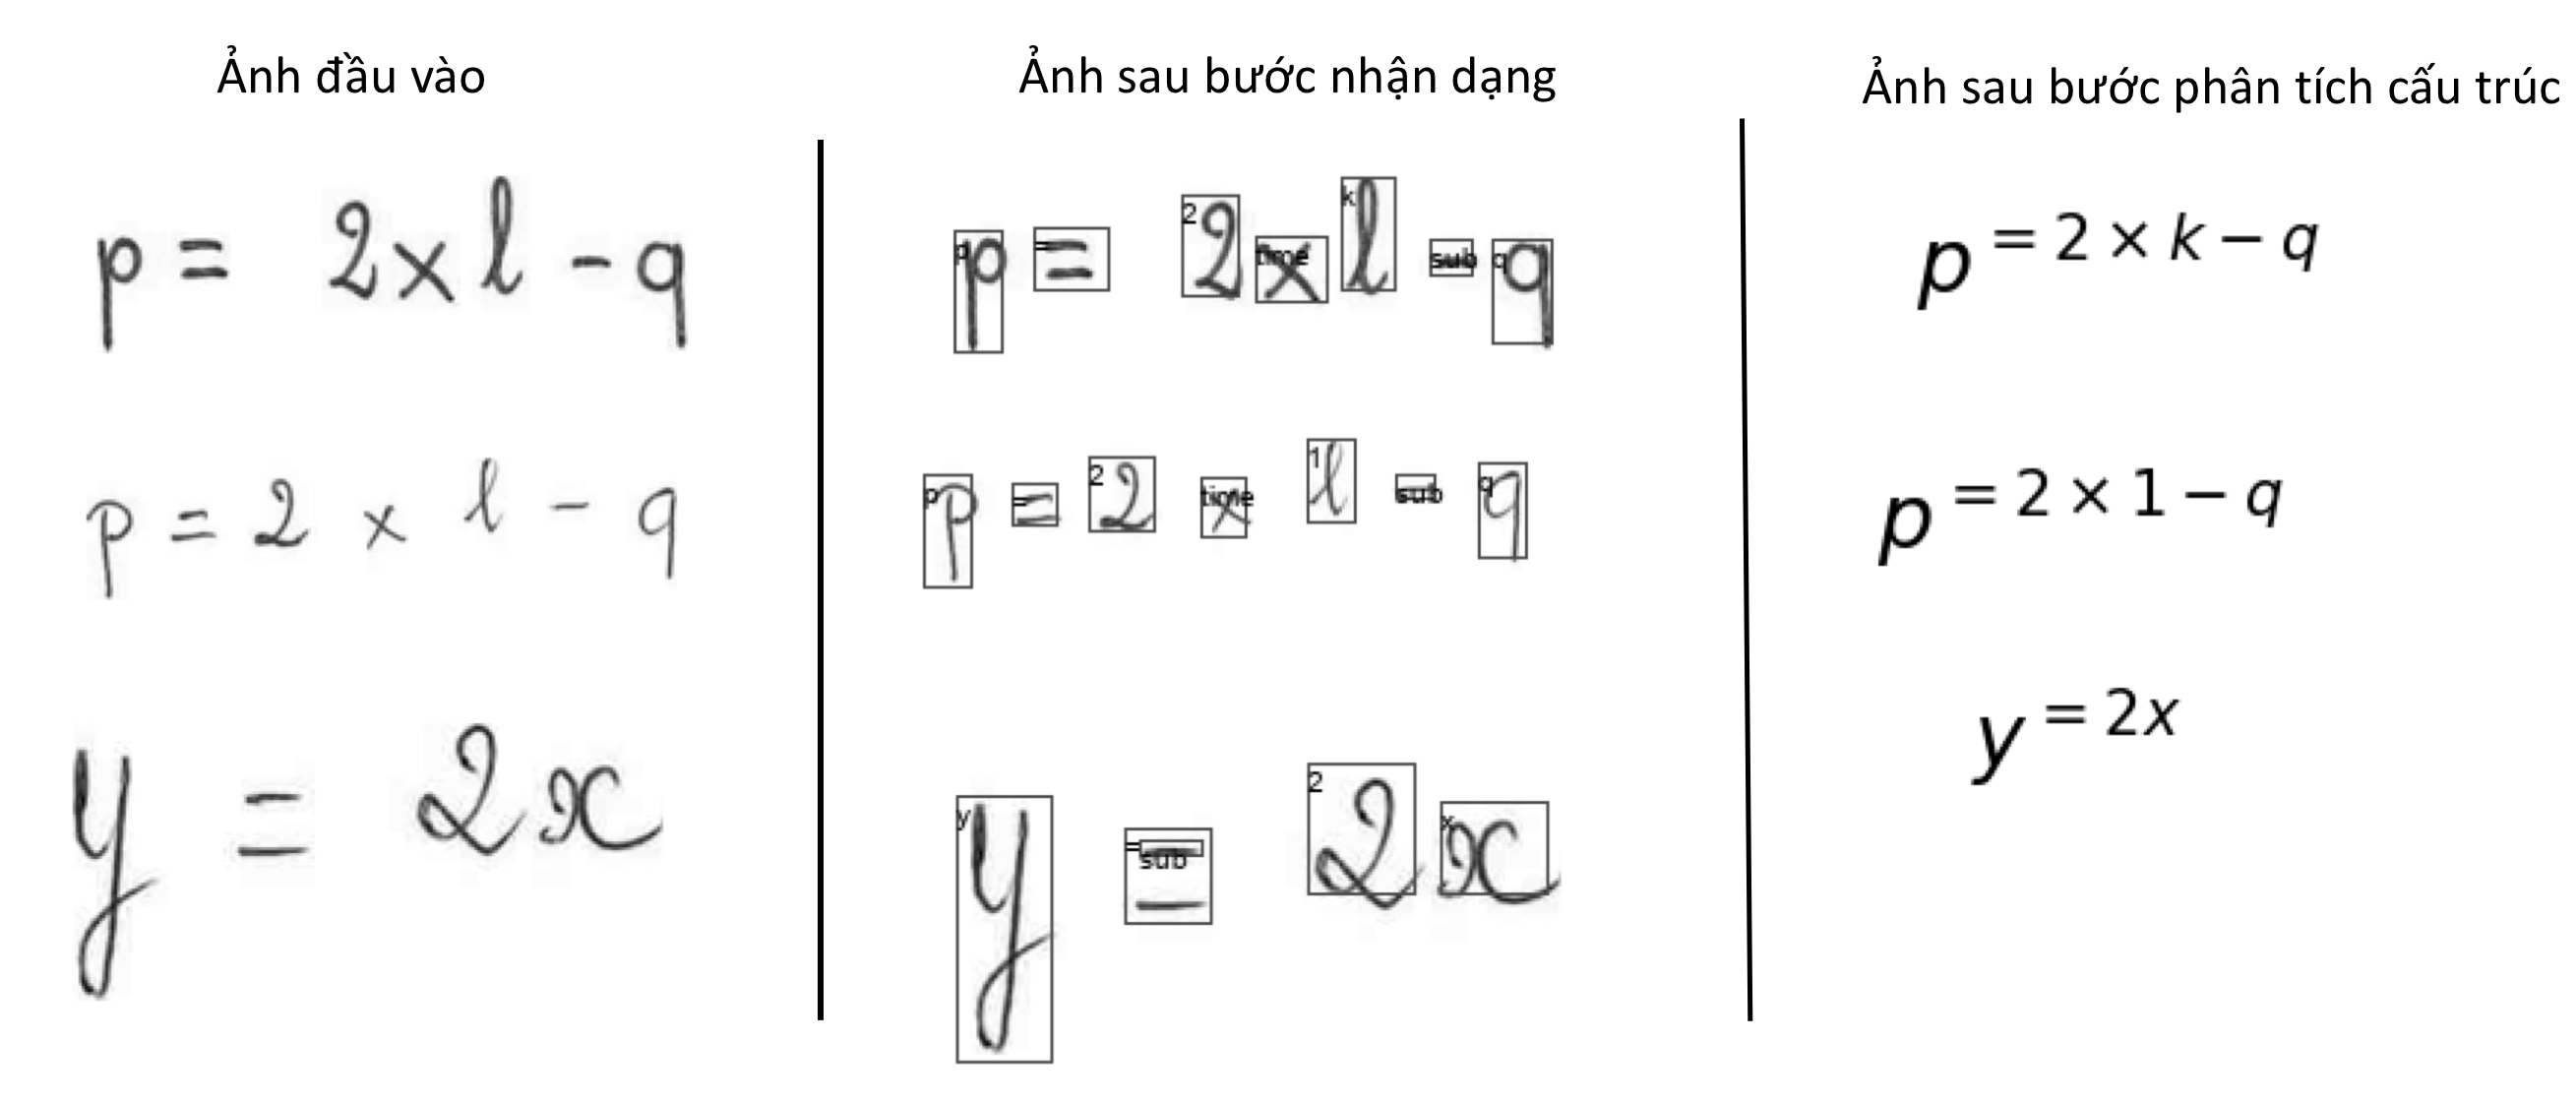
\includegraphics[width=0.775\linewidth]{phuluc_loi}
		\vspace{0.5cm}
		\captionof{figure}{Trường hợp sinh chuỗi Latex sai khi biểu thức chứa các ký tự có chân.}
	\end{center}
		\begin{center}
		\centering
		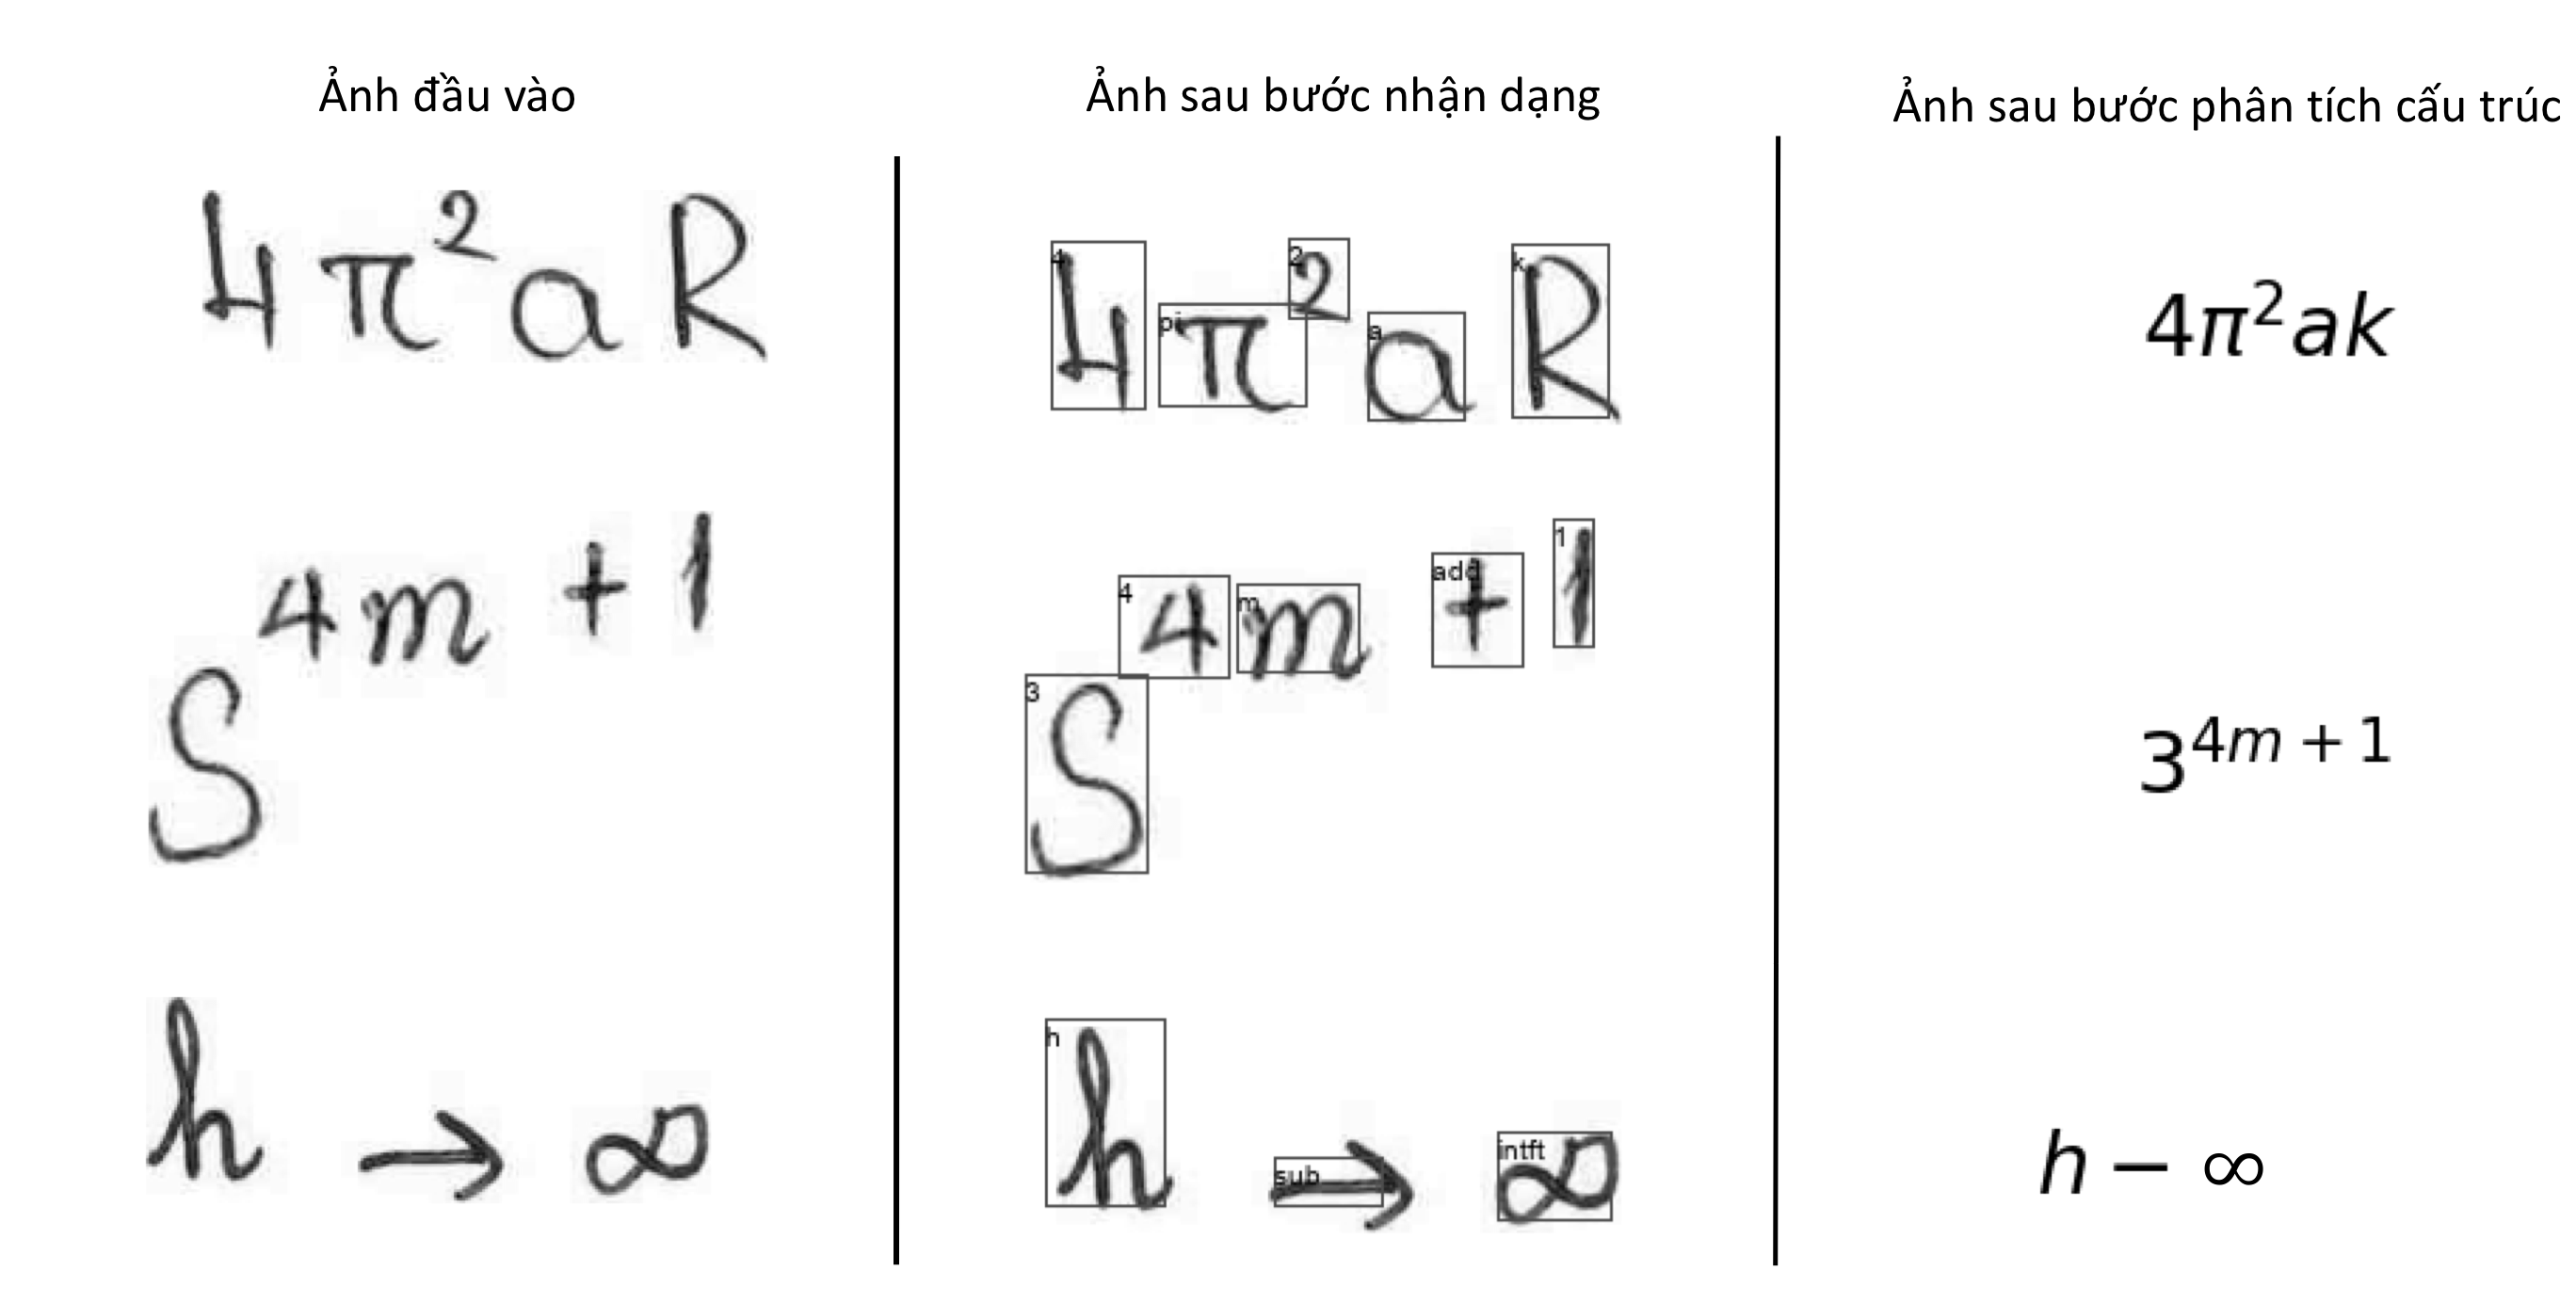
\includegraphics[width=0.775\linewidth]{phuluc_sainhan}
		\vspace{0.5cm}
		\captionof{figure}{Trường hợp hệ thống gán sai nhãn cho những ký tự có nét tương tự nhau.}
	\end{center}
	\newpage
	\bibliographystyle{ieeetr}
	\bibliography{ref}
\end{document}






